% Copyright 2004 by Till Tantau <tantau@users.sourceforge.net>.
%
% In principle, this file can be redistributed and/or modified under
% the terms of the GNU Public License, version 2.
%
% However, this file is supposed to be a template to be modified
% for your own needs. For this reason, if you use this file as a
% template and not specifically distribute it as part of a another
% package/program, I grant the extra permission to freely copy and
% modify this file as you see fit and even to delete this copyright
% notice. 

%%%%% DOCUMENT CLASS %%%%%
% Alternatively Comment/Uncomment these two lines 
% to print out the slides without pause
\documentclass{beamer}
%\documentclass[handout]{beamer}

%%%%%%%%%%%%%%%%%%%%%%%
%%%%% THEME BEGIN %%%%%
% There are many different themes available for Beamer. A comprehensive
% list with examples is given here:
% http://deic.uab.es/~iblanes/beamer_gallery/index_by_theme.html
% You can uncomment the themes below if you would like to use a different
% one:
%\usetheme{AnnArbor}
%\usetheme{Antibes}
%\usetheme{Bergen}
%\usetheme{Berkeley}
%\usetheme{Berlin}
%\usetheme{Boadilla}
%\usetheme{boxes}
%\usetheme{CambridgeUS}
%\usetheme{Copenhagen}
%\usetheme{Darmstadt}
%\usetheme{default}
%\usetheme{Frankfurt}
%\usetheme{Goettingen}
%\usetheme{Hannover}
%\usetheme{Ilmenau}
%\usetheme{JuanLesPins}
%\usetheme{Luebeck}
%\usetheme{Madrid}
%\usetheme{Malmoe}
%\usetheme{Marburg}
%\usetheme{Montpellier}
%\usetheme{PaloAlto}
%\usetheme{Pittsburgh}
%\usetheme{Rochester}
%\usetheme{Singapore}
%\usetheme{Szeged}
%\usetheme{Warsaw}

%%%%% CAL POLY COLOR DEFINITIONS
%\usepackage{calpolycolors}
\usetheme{CalPoly}

%%%%% CHANGING CRAP
%\usepackage{fontspec}
%\setmainfont{Avenir}
%%%%% THEME END %%%%%
%%%%%%%%%%%%%%%%%%%%%

%%%%% PACKAGES %%%%%
\usepackage{nth}
\usepackage{hyperref}

\usepackage{graphicx}
\usepackage{color, colortbl}
\usepackage{xcolor}
\definecolor{cpgreen}{HTML}{0A7951}
\definecolor{cpgold}{HTML}{FADA5E}
\definecolor{cpgreengold}{HTML}{82AA58}

%\usepackage{CJKutf8}

\usepackage{ifthen}
\usepackage{calc}
\usepackage{tikz}
\usetikzlibrary{decorations.pathreplacing, positioning, arrows.meta}
\usetikzlibrary{backgrounds}
  \tikzset{
    invisible/.style={opacity=0},
    visible on/.style={alt=#1{}{invisible}},
    alt/.code args={<#1>#2#3}{%
      \alt<#1>{\pgfkeysalso{#2}}{\pgfkeysalso{#3}} % \pgfkeysalso doesn't change the path
    },
  }

\usepackage{caption}
\usepackage{subcaption}

\usepackage{pgfplots}
\pgfplotsset{compat=1.3}

\usepackage{array}
\newcolumntype{L}[1]{>{\raggedright\let\newline\\\arraybackslash\hspace{0pt}}m{#1}}
\newcolumntype{C}[1]{>{\centering\let\newline\\\arraybackslash\hspace{0pt}}m{#1}}
\newcolumntype{R}[1]{>{\raggedleft\let\newline\\\arraybackslash\hspace{0pt}}m{#1}}

%%%%% COLORS
%\usepackage{xcolor}
\definecolor{cpgreen}{HTML}{0A7951}
\definecolor{cpgold}{HTML}{FADA5E}

\makeatletter
\def\rowcolor{\noalign{\ifnum0=`}\fi\bmr@rowcolor}
\newcommand<>{\bmr@rowcolor}{%
    \alt#1%
        {\global\let\CT@do@color\CT@@do@color\@ifnextchar[\CT@rowa\CT@rowb}% 
        {\ifnum0=`{\fi}\@gooble@rowcolor}% 
}

\newcommand{\@gooble@rowcolor}[2][]{\@gooble@rowcolor@}
\newcommand{\@gooble@rowcolor@}[1][]{\@gooble@rowcolor@@}
\newcommand{\@gooble@rowcolor@@}[1][]{\ignorespaces}
\makeatother

%%%%% CUSTOM MACROS %%%%%
\usepackage{cplop}

%%%%% TITLE/SUBTITLE %%%%%%
\title[Investigating The \krap{} And Clustering For \bs{}]{Investigating The \kraplong{} And Clustering For \BSlongs{}}
\subtitle{Exploring Two \MSTlong{} Methodologies}

%%%%% AUTHOR/INSTITUTE %%%%%%
\author{Jeffrey D. McGovern}
\institute{
  \textbf{\cplong{}}
  \\
  Computer Science and Software Engineering Department
}
%%%%% DATE/CONFERENCE %%%%%%
\date[March \nth{21} 2016]{Master's Thesis Defense\\March \nth{21} 2016}

%%%%% SUBJECT KEYWORDS %%%%%%
% Doesn't actually show up on the slides anywhere
\subject{\MSTlong{}}

%%%%% RECURRING LOGO %%%%%%
\pgfdeclareimage[height=0.5cm]{university-logo}{cp-logo-lrg}
\logo{\pgfuseimage{university-logo}}

%%%%% SHOW TABLE CONTENTS %%%%%
% This block creates a slide right when a new subsection starts.
% Comment or delete this block to remove this feature.
\AtBeginSection[]{
\begin{frame}<beamer>{Outline}
\small
    \tableofcontents[currentsection,currentsubsection]
\end{frame}
}
\AtBeginSubsection[]{
\begin{frame}<beamer>{\insertsection}{\insertsubsection}

\centering
\Large
\bfseries

\insertsection

\insertsubsection
\end{frame}
}

%%%%%%%%%%%%%%%%%%%%%%%%%%
%%%%% BEGIN DOCUMENT %%%%%
\begin{document}

% SOME DIAGRAMS REQUIRE THIS
\newsavebox\chickenFiveOne
\begin{lrbox}{\chickenFiveOne}
\begin{tikzpicture}[scale=0.5]
\begin{axis}[xticklabels={,,}, yticklabels={,,}, ticks=none, width=3in, height=1in]
\addplot[ybar interval=1, color=cpgreen, fill=cpgreen] 
table [col sep=comma] {data/pyroprints/ck005/4063.csv};
\end{axis}
\end{tikzpicture}
\end{lrbox}

\newsavebox\chickenFiveTwo
\begin{lrbox}{\chickenFiveTwo}
%\resizebox {3in} {1in} {
\begin{tikzpicture}[scale=0.5]
\begin{axis}[xticklabels={,,}, yticklabels={,,}, ticks=none, width=3in, height=1in]
\addplot[ybar interval=1, color=cpgold, fill=cpgold] 
table [col sep=comma] {data/pyroprints/ck005/4039.csv};
\end{axis}
\end{tikzpicture}
\end{lrbox}

\newsavebox\chickenSevenOne
\begin{lrbox}{\chickenSevenOne}
%\resizebox {3in} {1in} {
\begin{tikzpicture}[scale=0.5]
\begin{axis}[xticklabels={,,}, yticklabels={,,}, ticks=none, width=3in, height=1in]
\addplot[ybar interval=1, color=cpgreen, fill=cpgreen] 
table [col sep=comma] {data/pyroprints/ck007/4065.csv};
\end{axis}
\end{tikzpicture}
\end{lrbox}

\newsavebox\chickenSevenTwo
\begin{lrbox}{\chickenSevenTwo}
\begin{tikzpicture}[scale=0.5]
\begin{axis}[xticklabels={,,}, yticklabels={,,}, ticks=none, width=3in, height=1in]
\addplot[ybar interval=1, color=cpgold, fill=cpgold] table [col sep=comma] {data/pyroprints/ck007/4041.csv};
\end{axis}
\end{tikzpicture}
\end{lrbox}

%%%%%%%%%%%%%%%%%%%%%%%%%%%%%%%%%%%%%%%%
\begin{frame}
  \titlepage
\end{frame}

%%%%%%%%%%%%%%%%%%%%%%%%%%%%%%%%%%%%%%%%
\begin{frame}{Overview}
\small
\tableofcontents
\end{frame}

%%%%%%%%%%%%%%%%%%%%%%%%%%%%%%%%%%%%%%%%
\section{Introduction}
%%%%%%%%%%%%%%%%%%%%%%%%%%%%%%%%%%%%%%%%
\begin{frame}
  \begin{figure}
      \centering
      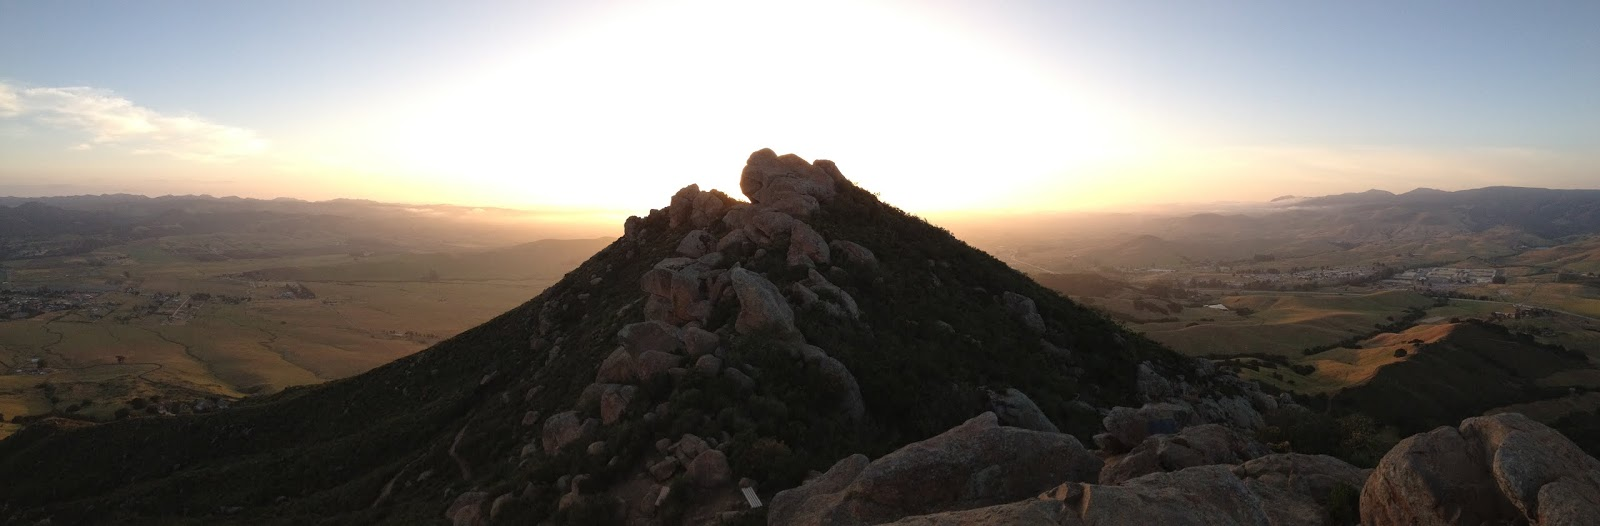
\includegraphics[width=\textwidth]{pics/bishops}
      \caption*{Bishop's Peak, San Luis Obispo, CA}
  \end{figure}
\end{frame}

%%%%%%%%%%%%%%%%%%%%%%%%%%%%%%%%%%%%%%%%
\begin{frame}
  \begin{figure}
      \centering
      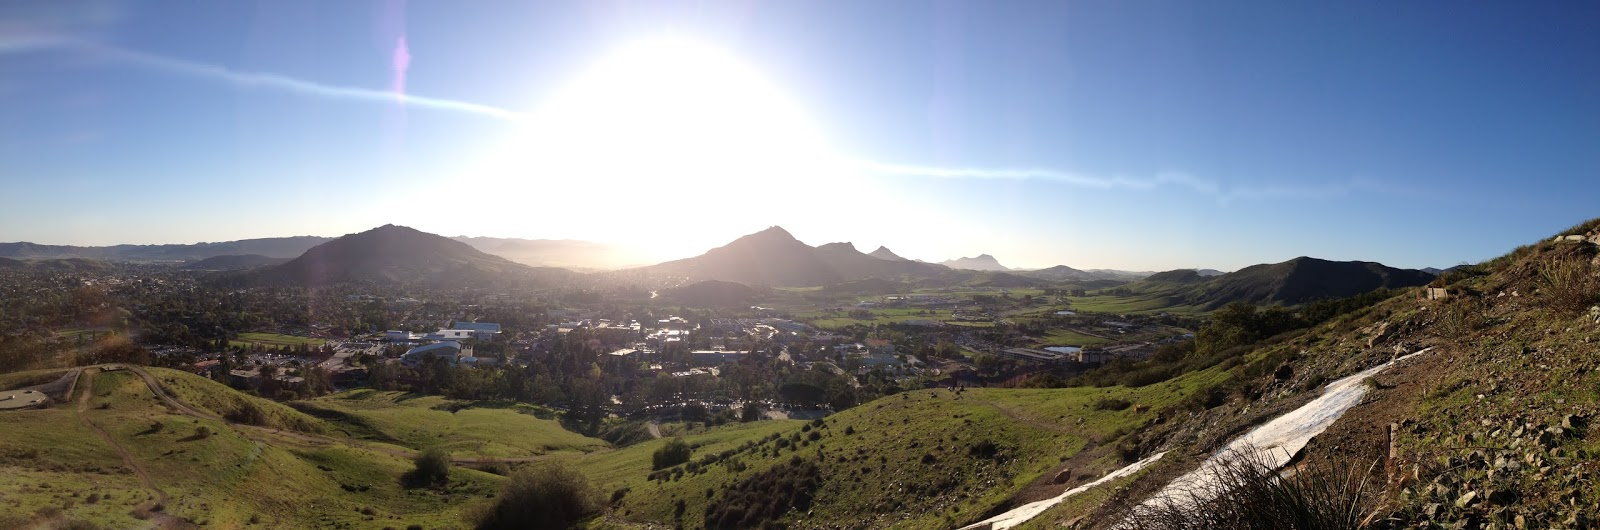
\includegraphics[width=\textwidth]{pics/seven_sisters}
      \caption*{Nine Sisters, San Luis Obispo, CA}
  \end{figure}
\end{frame}

%%%%%%%%%%%%%%%%%%%%%%%%%%%%%%%%%%%%%%%%
% MADONNA MOUNTAIN
\begin{frame}
  \begin{figure}
      \centering
      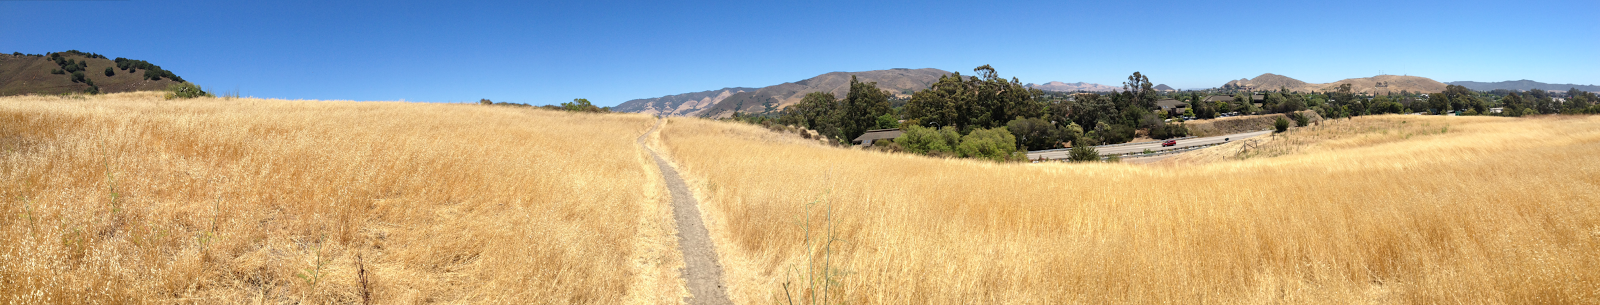
\includegraphics[width=\textwidth]{pics/field}
      \caption*{Madonna Mountain / Cerro San Luis Obispo}
  \end{figure}
\end{frame}

%%%%%%%%%%%%%%%%%%%%%%%%%%%%%%%%%%%%%%%%
% AVILA BEACH
\begin{frame}
  \begin{figure}
      \centering
      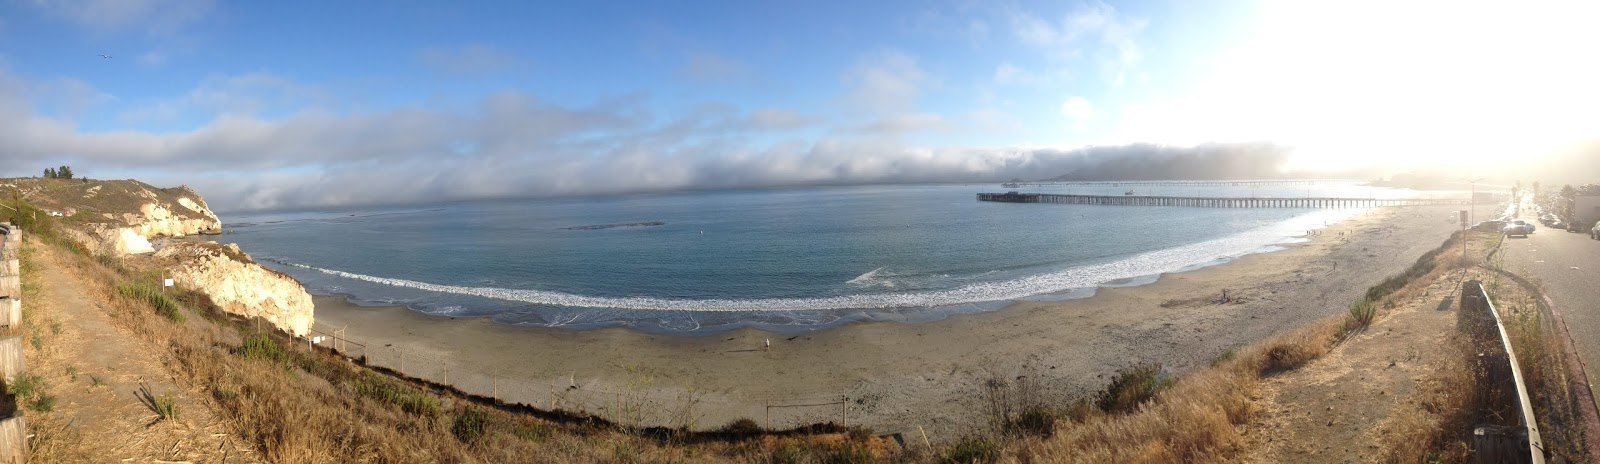
\includegraphics[width=\textwidth]{pics/avila}
      \caption*{Avila Beach, CA}
  \end{figure}
\end{frame}

%%%%%%%%%%%%%%%%%%%%%%%%%%%%%%%%%%%%%%%%
% BEACH CLOSED
\begin{frame}
\begin{center}
\begin{tikzpicture}
  \node (img1) {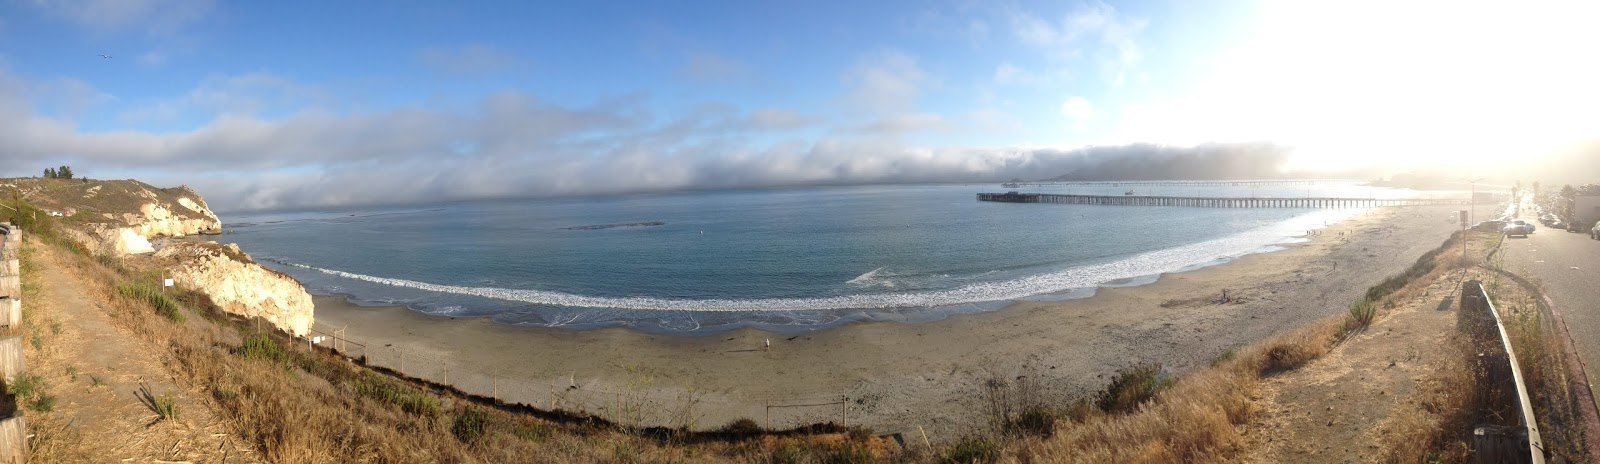
\includegraphics[width=\textwidth]{pics/avila}};
  %\pause
  \node[above left of=img1]  (img2) [xshift=-2cm]
  {
\includegraphics[height=3cm]{pics/closed1}};
  \pause
  \node[below right of=img1] (img3) [xshift=2cm]
  {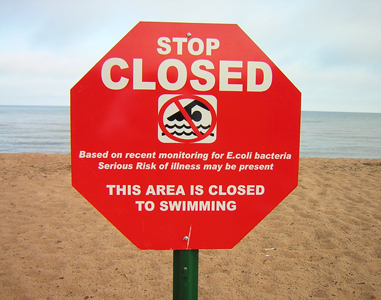
\includegraphics[height=3cm]{pics/closed3}};
    \pause
  \node[above right of=img1] (img3) [xshift=2cm]
  {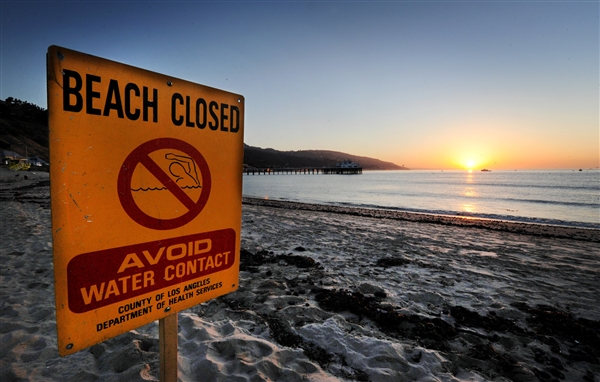
\includegraphics[height=3cm]{pics/closed2}};
    \pause
  \node[below left of=img1]  (img2) [xshift=-1.35cm]
  {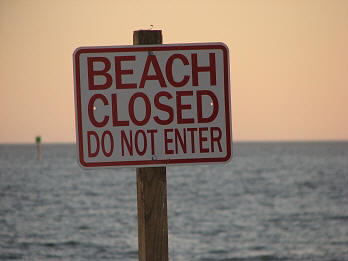
\includegraphics[height=3cm]{pics/closed4}};
\end{tikzpicture}
\end{center}
\end{frame}

%%%%%%%%%%%%%%%%%%%%%%%%%%%%%%%%%%%%%%%%
% FECAL INDICATOR BACTERIA
\begin{frame}
\centering
\begin{tikzpicture}
  \node (img1) {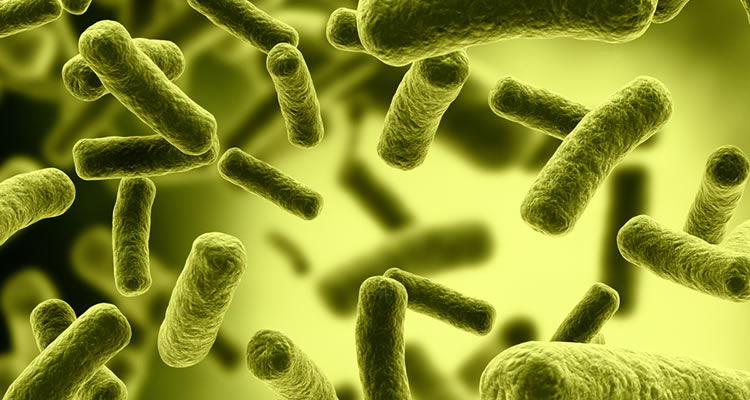
\includegraphics[width=\textwidth]{pics/ecoli}};
  \pause
  \node (img2) [fill=white]
  {\Huge \textbf{Who Pooped?}};
  \pause
  \node (img3) {
\includegraphics[height=0.80\textheight]{figures/poo}};
\end{tikzpicture}
\end{frame}

%%%%%%%%%%%%%%%%%%%%%%%%%%%%%%%%%%%%%%%%
%\subsection{Fecal Contamination}
%%%%%%%%%%%%%%%%%%%%%%%%%%%%%%%%%%%%%%%%
\begin{frame}{Fecal Contamination}{Problems}
{\Large Problems}
\begin{itemize}
    \item Dangerous for humans, animals, and ecosystems
    \begin{itemize}
        \item Bacteria, viruses, and bacteriophages can cause illness
        \item Certain bacteria can affect dissolved oxygen levels, harming aquatic life
        \item Removing bacteria with chemicals can harm aquatic life
    \end{itemize}
    \item Affects public and environmental water supplies
    \begin{itemize}
        \item Rivers
        \item Creeks
        \item Reservoirs
        \item Lakes
        \item Beaches
    \end{itemize}
    \item Common Solution:
    \begin{itemize}
        \item Restrict access
    \end{itemize}
\end{itemize}
\end{frame}
%%%%%%%%%%%%%%%%%%%%%%%%%%%%%%%%%%%%%%%%
\begin{frame}{Fecal Contamination}{Sources}
{\Large Sources}
\begin{itemize}
    \item Understanding the source is the first step to eliminating current and preventing further contamination
    \item Contaminants come from many different sources
    \begin{itemize}
        \item Wildlife
        \item Livestock
        \item Pets
        \item Humans
    \end{itemize}
\end{itemize}
\end{frame}

%%%%%%%%%%%%%%%%%%%%%%%%%%%%%%%%%%%%%%%%
\subsection{\MSTlong{}}
%%%%%%%%%%%%%%%%%%%%%%%%%%%%%%%%%%%%%%%%
\begin{frame}{\MSTlong{}}
\begin{block}{\MSTlong{}}
    Any technique that aims to discover the source \spec{} of biological matter using microbiological lifeforms.
\end{block}
\visible<2->{
\begin{itemize}
    \item Reliable Fecal Indicator Microbe
    \visible<3->{
    \begin{itemize}
        \item \FIBlong{} (\fib{}) e.g.:
        \begin{itemize}
            \item \enterococcus{}
            \item \bacteroides{}
            \item \ecolilong{} (\ecoli{})
        \end{itemize}
    \end{itemize}
    }
    \item Characteristic Representation
    \visible<4->{
    \begin{itemize}
        \item Phenotypic
        \item Genotypic
    \end{itemize}
    }
    \item Sourcing Methodology
    \visible<5->{
    \begin{itemize}
        \item \LibInd{}
        \item \LibDep{}
    \end{itemize}
    }
\end{itemize}
}
\end{frame}
%%%%%%%%%%%%%%%%%%%%%%%%%%%%%%%%%%%%%%%%
%\begin{frame}{\MSTlong{}}{Methodologies}
%\begin{itemize}
%    \item \LibInd{}
%    \begin{itemize}
%        \item Detects certain \fib{} that are known to be unique to particular \spec{}
%        \item \alert{Usually limited to humans and domesticated animals}
%    \end{itemize}
%    \item \LibDep{}
%    \begin{itemize}
%        \item Researchers build a library of known \spec{} \fib{}
%        \item Very flexible --- works for many \spec{}
%        \item \alert{Takes considerable effort to build}
%    \end{itemize}
%\end{itemize}
%\end{frame}

%%%%%%%%%%%%%%%%%%%%%%%%%%%%%%%%%%%%%%%%
\subsection{\cploplong{}}
%%%%%%%%%%%%%%%%%%%%%%%%%%%%%%%%%%%%%%%%
\begin{frame}{\cplop{}}{\cploplong{}}
\begin{center}
\begin{tikzpicture}
  \node (proc1) 
  {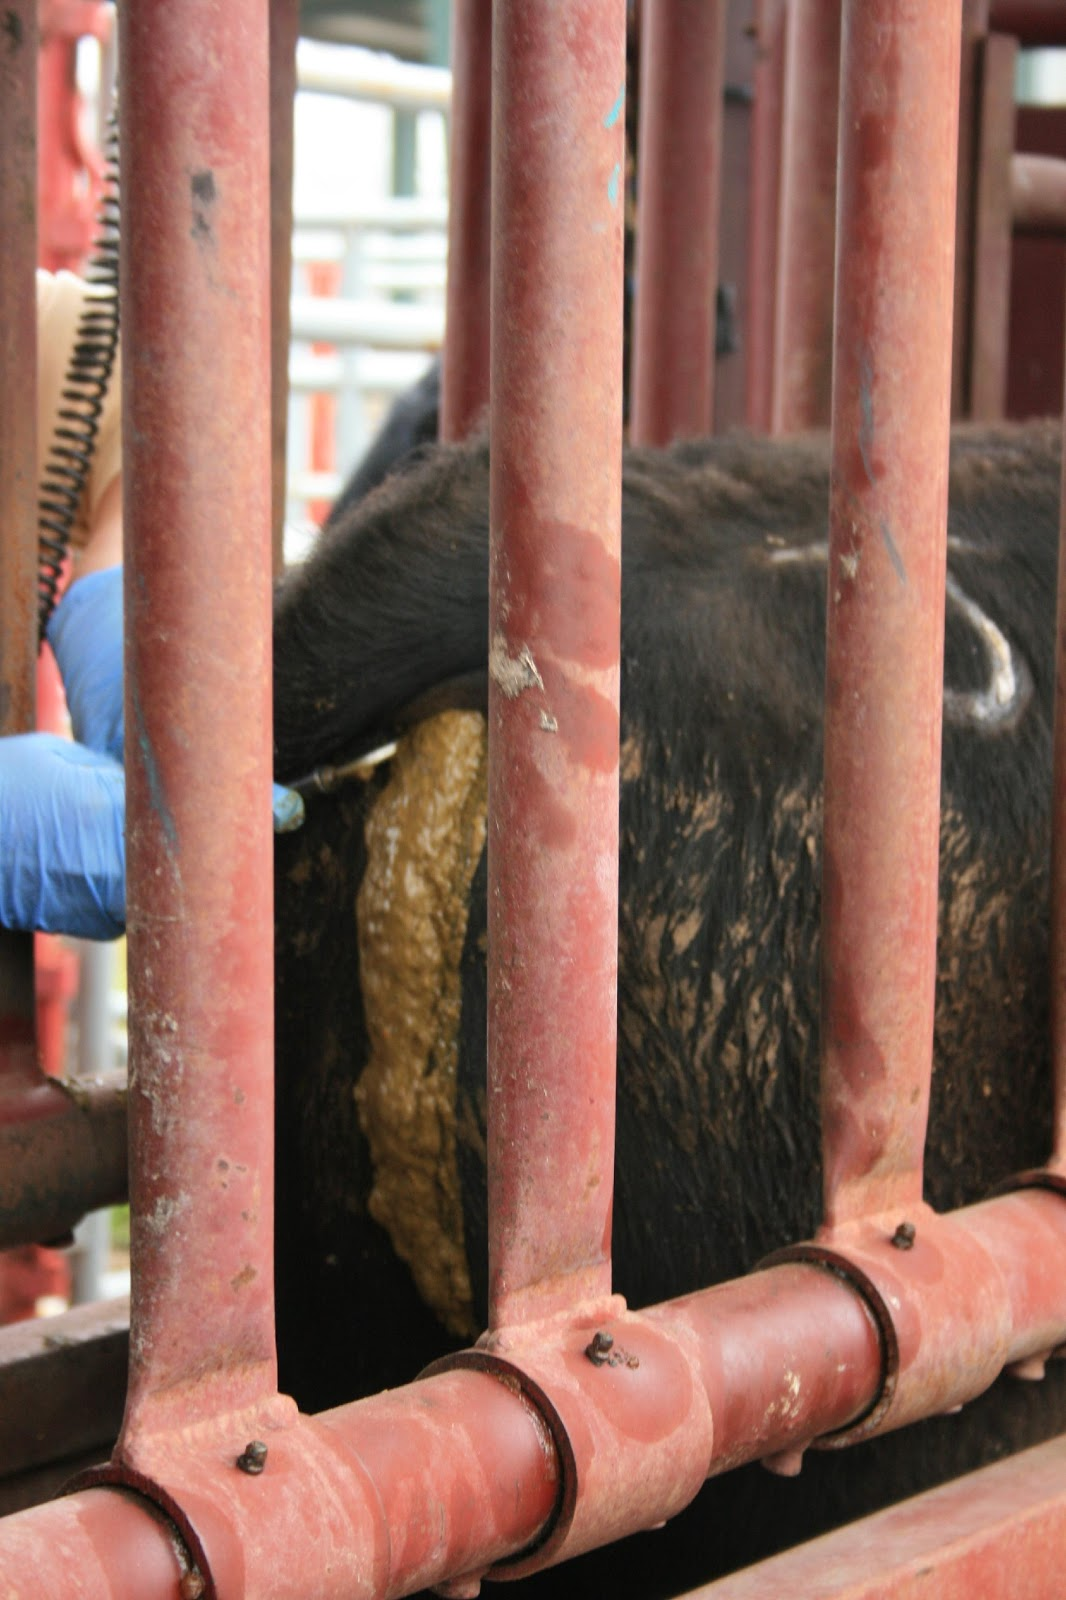
\includegraphics[width=2.5cm]{pics/process1}};
  \node[right of=proc1] (proc4) [xshift=1cm]
  {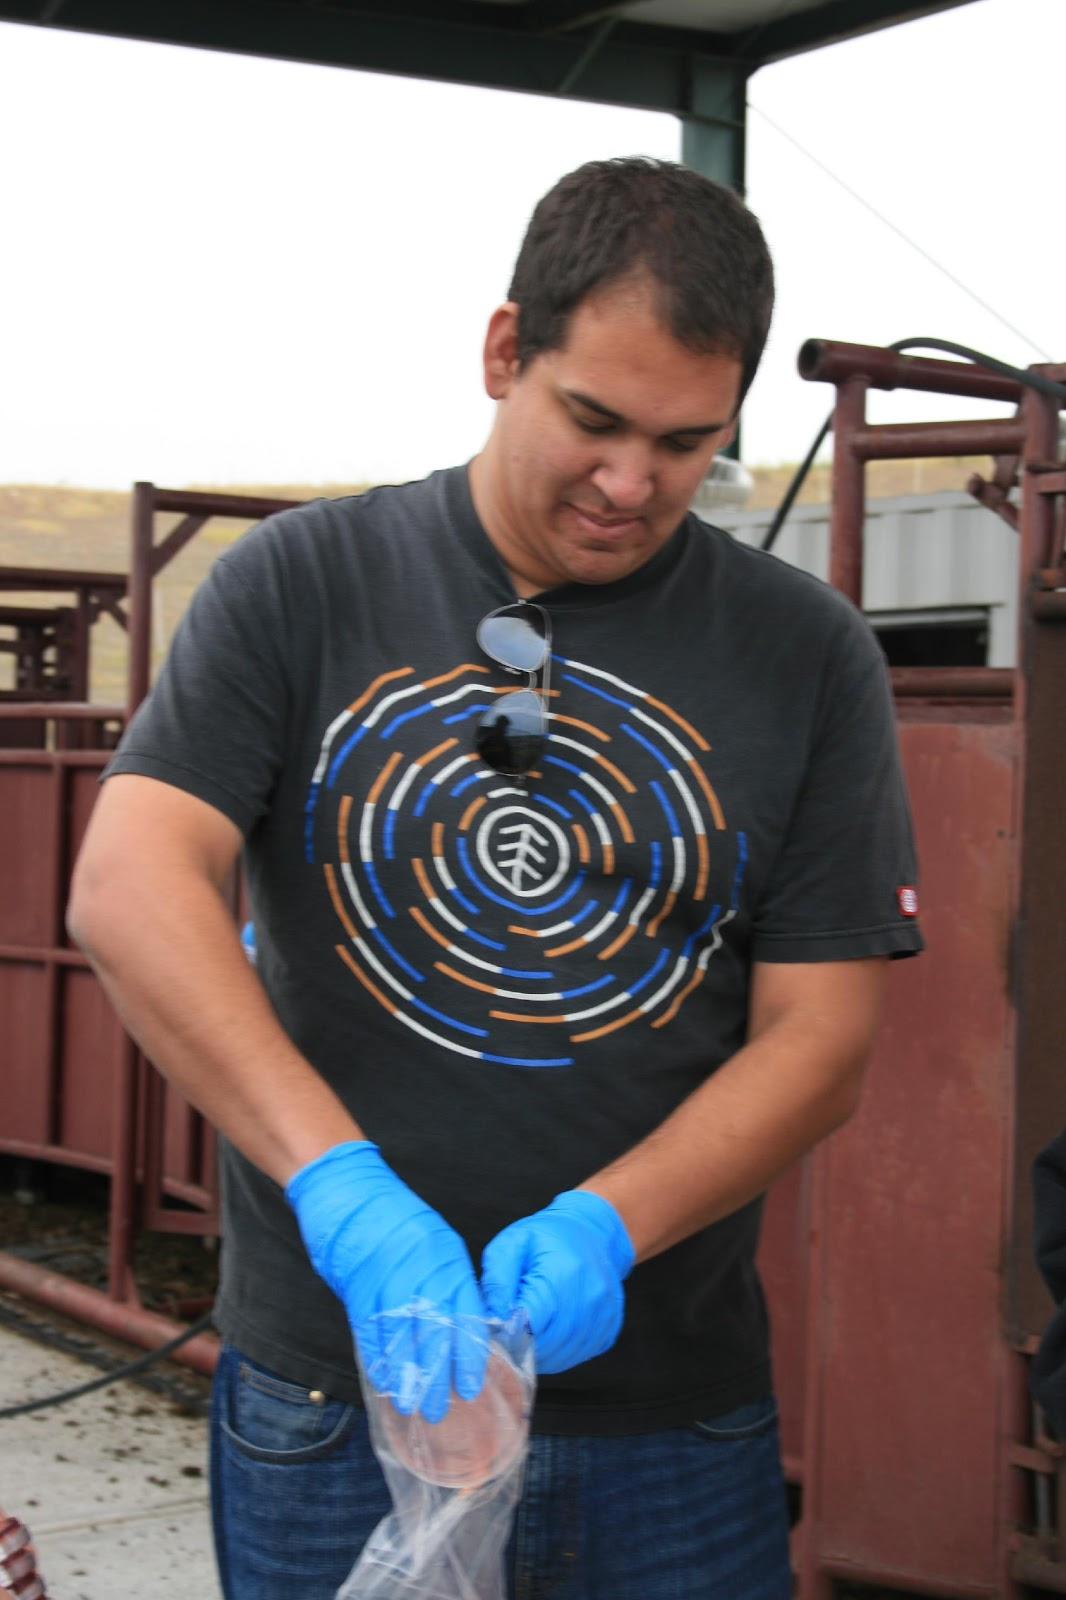
\includegraphics[width=2.5cm]{pics/process4}};

  \node[right of=proc4] (img1) [xshift=3.5cm]
  {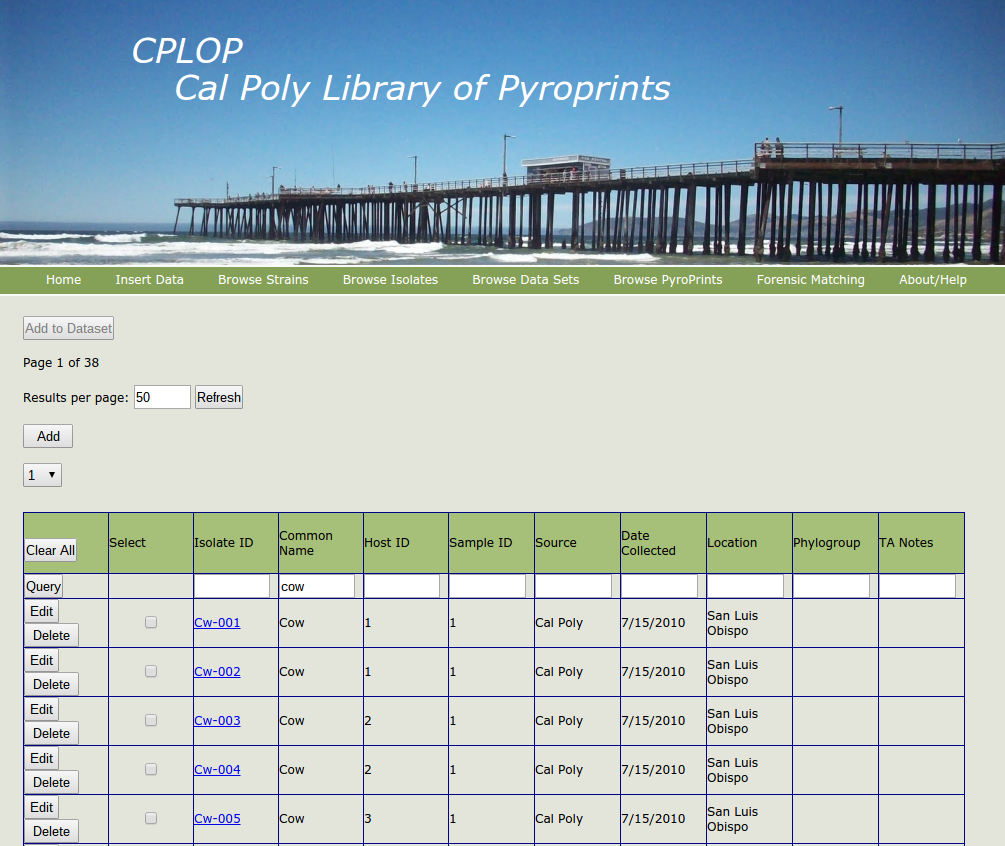
\includegraphics[width=4cm]{pics/cplop1}};
  \node[below right of=img1]  (img2) [yshift=-1cm, xshift=.5cm]
  {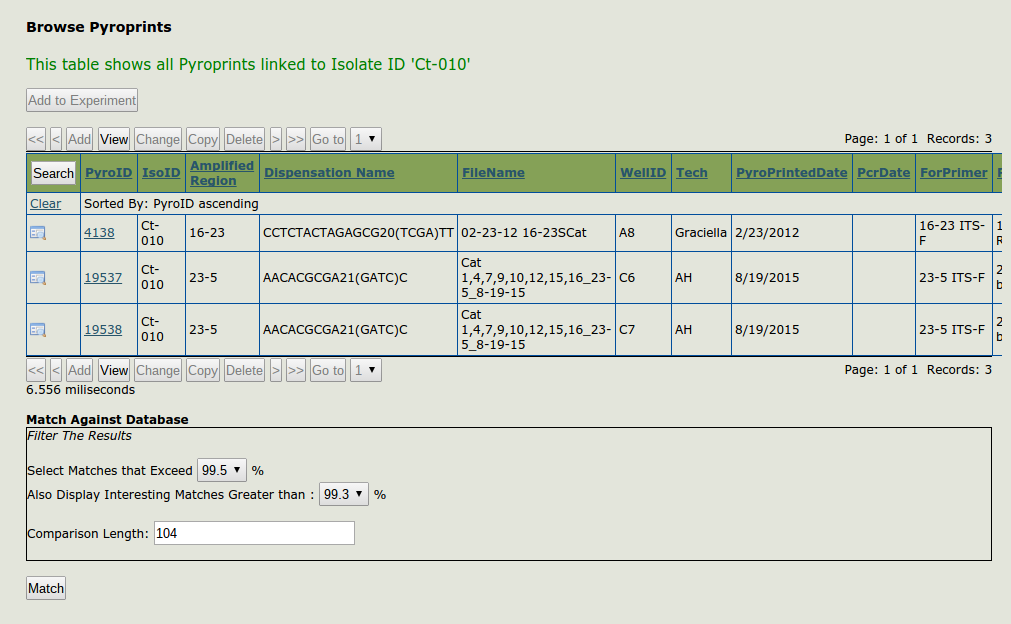
\includegraphics[width=4cm]{pics/cplop2}};
  \node[below right of=img2] (img3)
  {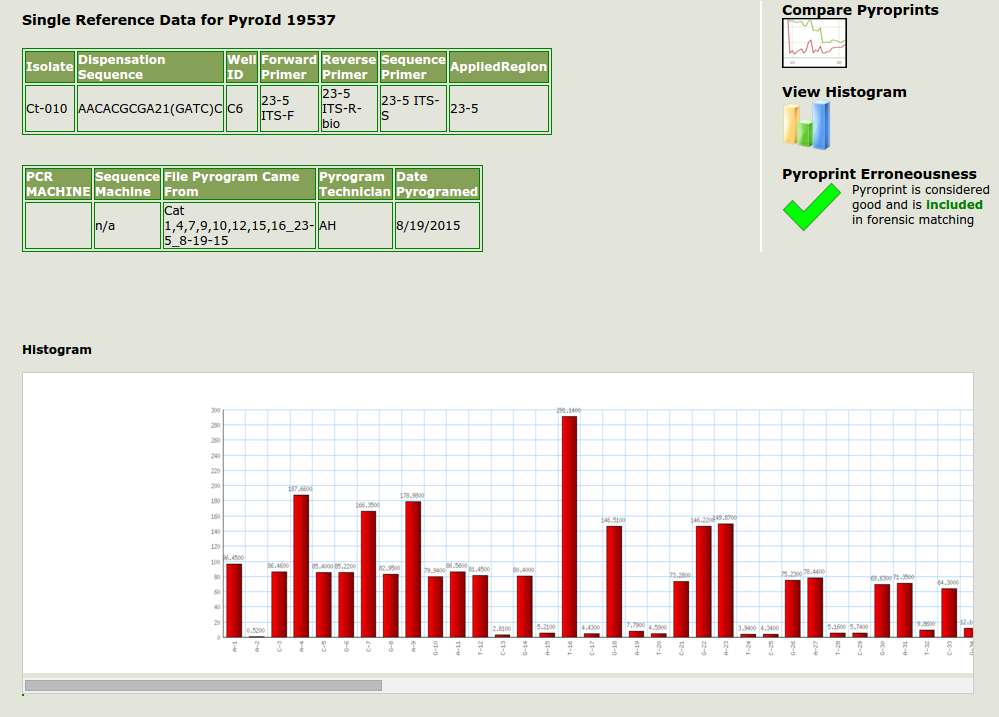
\includegraphics[width=4cm]{pics/cplop3}};
  
  \draw[-{>[scale=2.5,
          length=2,
          width=6]},line width=1pt] (proc4) to (img1);
\end{tikzpicture}
\end{center}
\end{frame}

%%%%%%%%%%%%%%%%%%%%%%%%%%%%%%%%%%%%%%%%
\begin{frame}{\cploplong{}}
\begin{block}{\cploplong{} (\cplop{})}
A database of \ecoli{} \dna{} pyrosequence fingerprints, called \textbf{\pyros{}}, built and maintained by \cp{} students and faculty.
\end{block}
\begin{itemize}
    \item Reliable Fecal Indicator Microbe
    \begin{itemize}
        \item \FIBlong{} (\fib{}) e.g.:
        \begin{itemize}
            \item \enterococcus{}
            \item \bacteroides{}
            \item \bfseries \ecolilong{} (\ecoli{})
        \end{itemize}
    \end{itemize}
    \item Characteristic Representation
    \begin{itemize}
        \item Phenotypic
        \item \bfseries Genotypic (\Pyros{})
    \end{itemize}
    \item Sourcing Methodology
    \begin{itemize}
        \item \LibInd{}
        \item \bfseries \LibDep{}
    \end{itemize}
\end{itemize}
\end{frame}
%%%%%%%%%%%%%%%%%%%%%%%%%%%%%%%%%%%%%%%%
%\subsection{\protect\textit{E. Coli} \Isols}
\subsection{Background}
%%%%%%%%%%%%%%%%%%%%%%%%%%%%%%%%%%%%%%%%
\begin{frame}{Building \cplop{}}
Process to build the \cplop{} library:
\begin{enumerate}
    \item Collect fecal samples from known \spec{}
    \item Culture individual (\ecoli{}) \isols{} from fecal matter
    \item Build a digital representation (\pyros{}) of the \isol{}
    \item Insert representation (\pyros{}) into \cplop{} database
\end{enumerate}
\begin{center}
Species $\leftarrow$
%
Host $\leftarrow$
%
Fecal Sample $\leftarrow$
%
\Isol{} $\leftarrow$
%
\Pyro{}
\end{center}
\end{frame}
%%%%%%%%%%%%%%%%%%%%%%%%%%%%%%%%%%%%%%%%
\begin{frame}[t]{\Isols{}}{Collecting Samples From Known \Spec{}}
\begin{center}
{\bfseries
Species $\leftarrow$
%
Host $\leftarrow$
%
Fecal Sample $\leftarrow$}
%
\Isol{} $\leftarrow$
%
\Pyro{}
\end{center}
\vfill
\centering
\begin{tikzpicture}
\node (proc1) 
{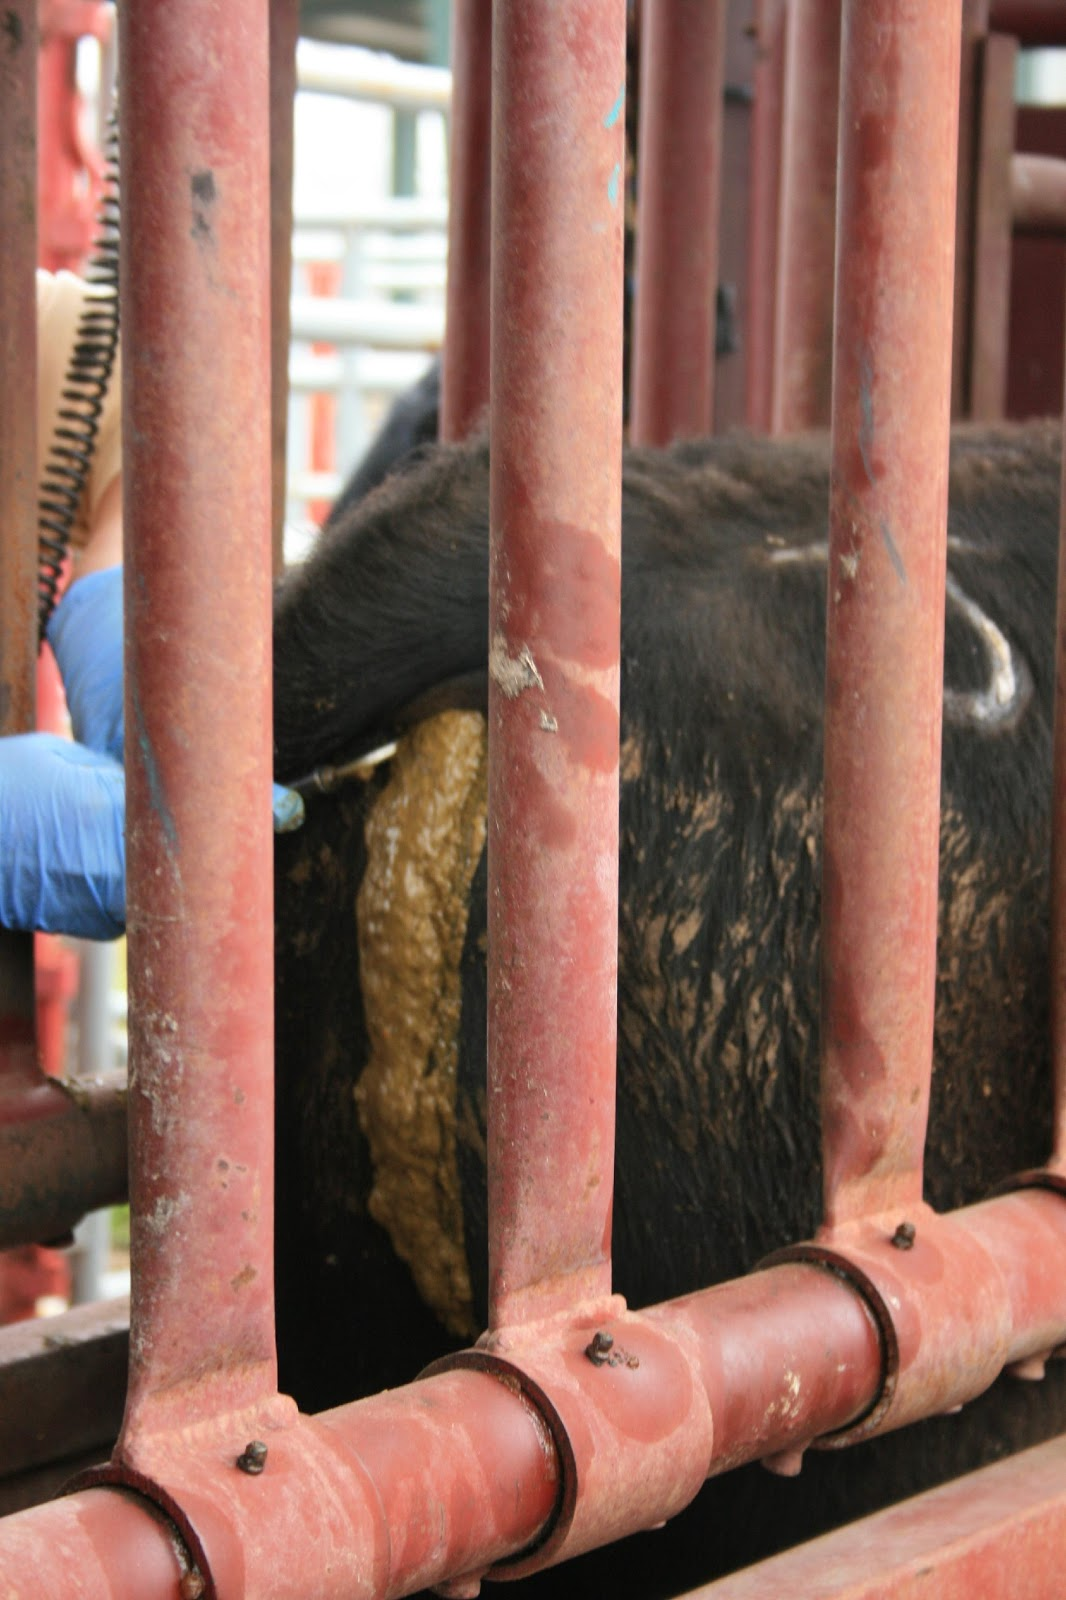
\includegraphics[width=3.5cm]{pics/process1}};
\node[right of=proc1] (proc4) [xshift=3.75cm]
{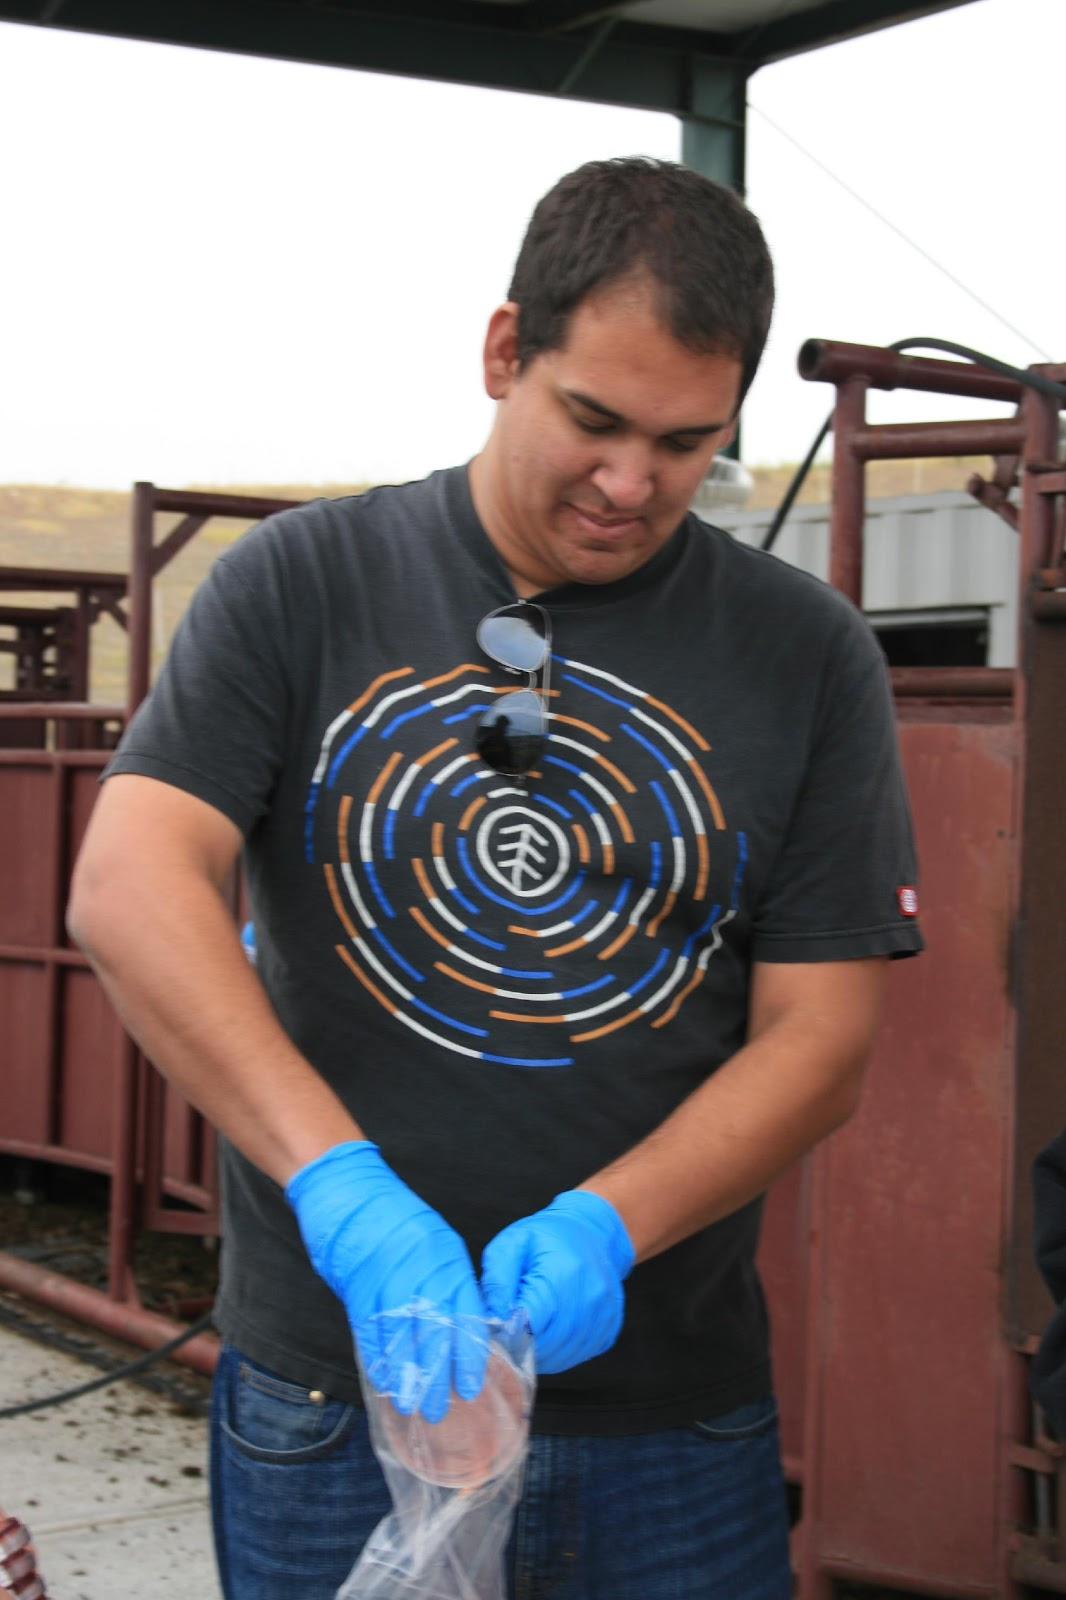
\includegraphics[width=3.5cm]{pics/process4}};
\end{tikzpicture}
\end{frame}

%%%%%%%%%%%%%%%%%%%%%%%%%%%%%%%%%%%%%%%%
\begin{frame}[t]{\Isols{}}{Culturing \ecoli{} \Isols{}}
\begin{center}
Species $\leftarrow$
%
Host $\leftarrow$
%
Fecal Sample $\leftarrow$
%
{\bfseries \Isol{} $\leftarrow$}
%
\Pyro{}
\end{center}
\begin{block}{\Isols{}}
An individual culture (of \ecoli{}) grown from a fecal sample.
\end{block}
\centering
\pause
\begin{tikzpicture}]
  \node (petri) at (0,0)
  {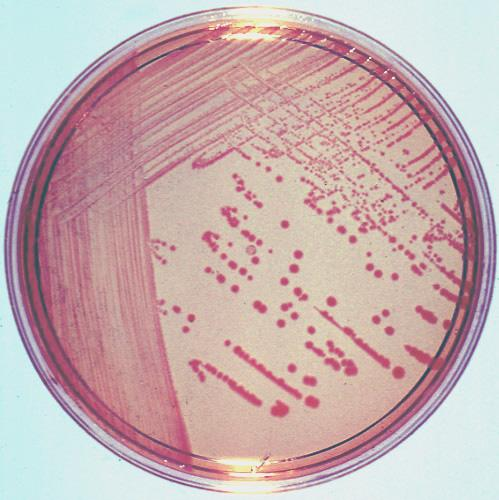
\includegraphics[width=4cm]{pics/petri}};
  
  \pause
  \node[left of=petri] (poo) [xshift=-3cm] {
\includegraphics[width=2.5cm]{figures/poo}};
  \path[->] (-3cm,-0.75cm) edge [bend right, line width=1pt] (-1.25,-0.04);
  
  \pause
  \node[above right of=petri] (isolate_text) [xshift=3cm, yshift=1cm]
  {\Isol{}};
  \path[->] (isolate_text) edge [bend left, line width=1pt] (.50,-0.04) ;
\end{tikzpicture}
\end{frame}

%%%%%%%%%%%%%%%%%%%%%%%%%%%%%%%%%%%%%%%%
% UNUSED
\newsavebox\greyBox
\begin{lrbox}{\greyBox}
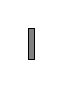
\begin{tikzpicture}[scale=0.04]
\draw[fill=gray] (-1,5)rectangle(1,-5);
\end{tikzpicture}
\end{lrbox}

\newsavebox\blackBox
\begin{lrbox}{\blackBox}

\begin{tikzpicture}[scale=0.04]
\draw[fill=black] (-1,5)rectangle(1,-5);
\end{tikzpicture}
\end{lrbox}

\newsavebox\region
\begin{lrbox}{\region}
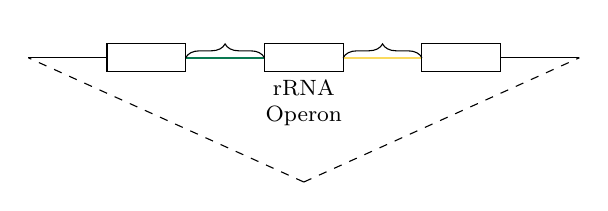
\begin{tikzpicture}

% Draw three filled circles for points a,x,b, and define 
% them as TikZ nodes
\footnotesize

\coordinate (a) at (0,0);
\coordinate (b) at (1,0);
\coordinate (c) at (2,0);
\coordinate (d) at (3,0);
\coordinate (e) at (4,0);
\coordinate (f) at (5,0);
\coordinate (g) at (6,0);
\coordinate (h) at (7,0);

% Label the points
\draw  (a) -- (b);
\draw[thick, color=cpgreen] (c)--(d);
\draw[thick, color=cpgold] (e)--(f);
\draw  (g) -- (h);
\draw[fill=white] (1,5pt)rectangle(2,-5pt) node[pos=.5]{\Gsixt{}};
\draw[fill=white] (3,5pt)rectangle(4,-5pt) node[pos=.5](gtwen){\Gtwen{}{}};
\draw[fill=white] (5,5pt)rectangle(6,-5pt) node[pos=.5]{\Gfive{}};


\node[below of=gtwen, text width=30, align=center, yshift=12pt] (rna) {rRNA Operon};
\coordinate[below of=rna] (bottom);

\draw[dashed](bottom)--(a);
\draw[dashed](bottom)--(h);

\draw[decorate,decoration={brace,amplitude=5pt}] (c) -- (d)
node [black,midway,above=5pt] {\Ssixt{}};
\draw[decorate,decoration={brace,amplitude=5pt}] (e) -- (f)
node [black,midway,above=5pt] {\Sfive{}};
\end{tikzpicture}
\end{lrbox}
%%%%%%%%%%%%%%%%%%%%%%%%%%%%%%%%%%%%%%%%
% SIMPLE DNA
\begin{frame}[t]{\Isols{}}{\ecoli{} \dna{}}
\begin{center}
Species $\leftarrow$
%
Host $\leftarrow$
%
Fecal Sample $\leftarrow$
%
{\bfseries \Isol{} $\leftarrow$}
%
\Pyro{}
\end{center}
\begin{figure}[ht]
  \centering
    \begin{tikzpicture}[scale=1]
        \coordinate (center) at (0,0);
        \draw (center) circle (1.5);
        \node (top) at (90:1.5) {\usebox\greyBox};
        \node[rotate around={170:(0,0)}] at (80:1.5) {\usebox\greyBox};
        \node[rotate around={10:(0,0)}] at (100:1.5) {\usebox\blackBox};
        \node[rotate around={20:(0,0)}] at (110:1.5) {\usebox\blackBox};
        \node[rotate around={30:(0,0)}] at (120:1.5) {\usebox\greyBox};
        \node[rotate around={90:(0,0)}] at (180:1.5) {\usebox\blackBox};
        \node[rotate around={160:(0,0)}] at (250:1.5) {\usebox\blackBox};
        \pause
        %\node[above of=top, yshift=8pt] {\usebox\region};
        
        \footnotesize

        \coordinate (a) at (-3.5,3.40);
        \coordinate (b) at (-2.5,3.40);
        \coordinate (c) at (-1.5,3.40);
        \coordinate (d) at ( -.5,3.40);
        \coordinate (e) at (  .5,3.40);
        \coordinate (f) at ( 1.5,3.40);
        \coordinate (g) at ( 2.5,3.40);
        \coordinate (h) at ( 3.5,3.40);
        
        % Label the points
        \draw  (a) -- (b);
        \draw[thick, color=cpgreen] (c)--(d);
        \draw[thick, color=cpgold] (e)--(f);
        \draw  (g) -- (h);
        \node (rect) at (-2,3.40) [draw, minimum width=1cm, minimum height=10pt, anchor=center] {\Gsixt{}};
        \node (gtwen) at (0,3.40) [draw, minimum width=1cm, minimum height=10pt, anchor=center] {\Gtwen{}};
        \node (rect) at (2,3.40) [draw, minimum width=1cm, minimum height=10pt, anchor=center] {\Gfive{}};
        
        \node[below of=gtwen, text width=30, align=center, yshift=8pt] (rna) {rRNA Operon};
        \coordinate[below of=rna] (bottom);
        
        \draw[dashed](bottom)--(a);
        \draw[dashed](bottom)--(h);
        
        \pause
        \draw[decorate,decoration={brace,amplitude=5pt}] (c) -- (d)
        node [black,midway,above=5pt] {\Ssixt{}};
        \draw[decorate,decoration={brace,amplitude=5pt}] (e) -- (f)
        node [black,midway,above=5pt] {\Sfive{}};
    \end{tikzpicture}  
    %\caption{\ecoli{} DNA, outlining the highly variable \Ssixt{} and \Sfive{} \itsshort{} regions, which repeat 7 times around the \ecoli{} genome.}
  \label{fig:regions_printed}
\end{figure}
\end{frame}

%%%%%%%%%%%%%%%%%%%%%%%%%%%%%%%%%%%%%%%%
\begin{frame}[t]{\ITSlongs{}}
\begin{center}
Species $\leftarrow$
%
Host $\leftarrow$
%
Fecal Sample $\leftarrow$
%
{\bfseries \Isol{} $\leftarrow$}
%
\Pyro{}
\end{center}
\begin{block}{\ITSlongs{} (\itsshort{})}
The two, highly variable regions of \dna{} between the \Gsixt{}, \Gtwen{}, and \Gfive{} genes in \ecoli{} and referred to as \Ssixt{} and \Sfive{}.
\end{block}
\begin{itemize}
    \item Do not code for functional products $\Rightarrow$ \textbf{highly variable}
    \item Any offspring of a microbe inherit \Ssixt{} and \Sfive{}
    \item Biologists to use them to differentiate between strains
\end{itemize}
\end{frame}

%%%%%%%%%%%%%%%%%%%%%%%%%%%%%%%%%%%%%%%%
%\subsection{\Pyros{}}
%%%%%%%%%%%%%%%%%%%%%%%%%%%%%%%%%%%%%%%%
\begin{frame}[t]{\Pyro{}}
\begin{center}
Species $\leftarrow$
%
Host $\leftarrow$
%
Fecal Sample $\leftarrow$
%
\Isol{} $\leftarrow$
%
{\bfseries \Pyro{}}
\end{center}
\begin{block}{\Pyro{}}
The peak light values of the pyrosequencing of one of the \itsshort{} regions in the seven loci of the \ecoli{} genome.
\end{block}
Process to build a \pyro{} from an \ecoli{} \isol{}:
\begin{itemize}
    \item Purify the \isol{}
    \item Amplify the \isol{}'s \itsshort{} region (using \pcr{})
    \item Pyrosequence the amplified \itsshort{} region
\end{itemize}
\end{frame}

%%%%%%%%%%%%%%%%%%%%%%%%%%%%%%%%%%%%%%%%
% PYRO PROCESS
\begin{frame}[t]{\ecoli{} \dna{}}{Pyroprinting Process}
\begin{center}
Species $\leftarrow$
%
Host $\leftarrow$
%
Fecal Sample $\leftarrow$
%
\Isol{} $\leftarrow$
%
{\bfseries \Pyro{}}
\end{center}
\begin{figure}[ht]
  \centering
  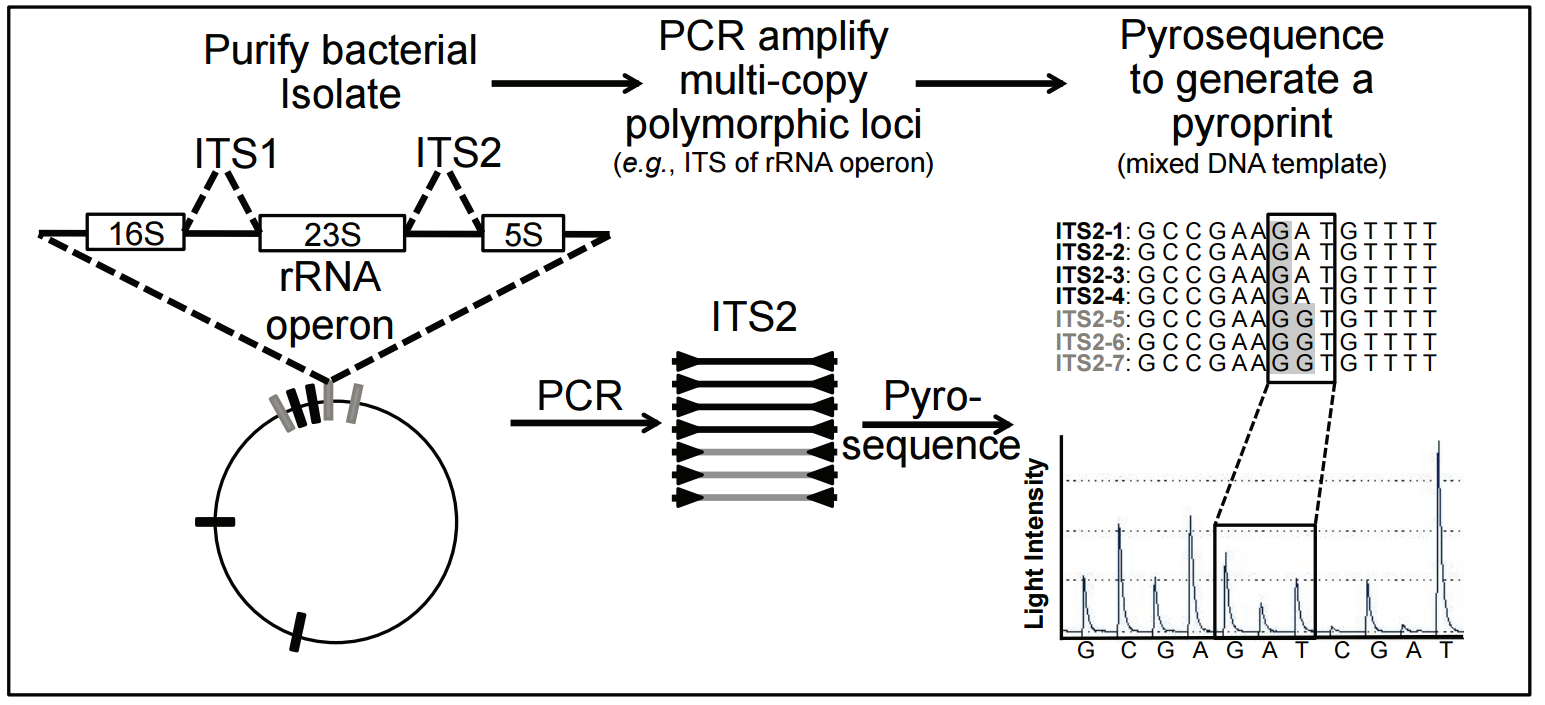
\includegraphics[width=\textwidth]{pics/pyro_process}
  \caption{The pyroprinting process of an isolate.}
\end{figure}
\end{frame}

%%%%%%%%%%%%%%%%%%%%%%%%%%%%%%%%%%%%%%%%
% HISTOGRAM
\begin{frame}[t]{Pyroprint}{Histogram Representation}
\begin{center}
Species $\leftarrow$
%
Host $\leftarrow$
%
Fecal Sample $\leftarrow$
%
\Isol{} $\leftarrow$
%
{\bfseries \Pyro{}}
\end{center}
\begin{center}
\begin{figure}
    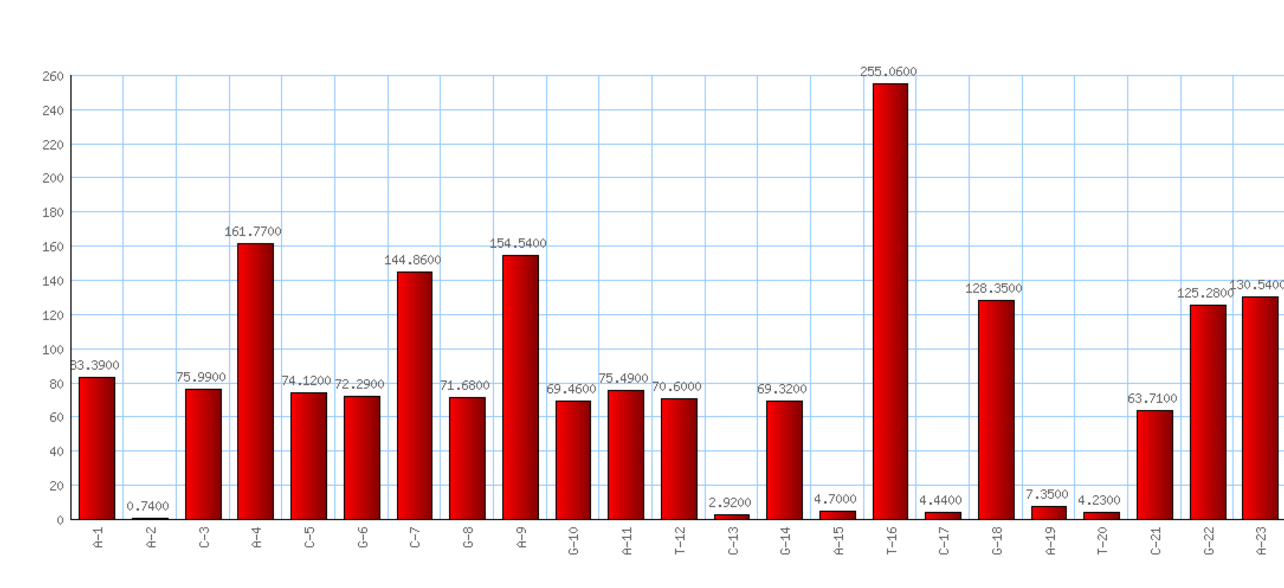
\includegraphics[width=\textwidth]{pics/pyro1}
\end{figure}
\end{center}
\end{frame}

%%%%%%%%%%%%%%%%%%%%%%%%%%%%%%%%%%%%%%%%
\begin{frame}[t]{Comparing Pyroprints}{\Pearson{}}
\begin{center}
Species $\leftarrow$
%
Host $\leftarrow$
%
Fecal Sample $\leftarrow$
%
\Isol{} $\leftarrow$
%
{\bfseries \Pyro{}}
\end{center}
\centering
{\Large \bfseries
\Pearson{}}
\vfill
\[
    \pcfunc{\pca{}}{\pcb{}}
    =
    %\pclong{\pcveca}{\pcvecb}
    \pceric{\pca{}}{\pcb{}}
    =
    \frac{\veccov{\pca{}}{\pcb{}}}{\vecstddev{\pca{}}\cdot\vecstddev{\pcb}}
    %\frac{cov(\vec{u},\vec{p})}{\sigma_{\vec{u}}\cdot %\sigma_{\vec{p}}} 
\]

\vfill
\raggedright
\Pearson{} Values:
\begin{itemize}
    \item Close to 1 $\Rightarrow$ highly similar
    \item Close to 0 $\Rightarrow$ completely dissimilar
    \item Close to -1 $\Rightarrow$ inversely similar
\end{itemize}
\raggedright

Always positive between any two \pyros{} in \cplop{}
\vfill
\end{frame}


%%%%%%%%%%%%%%%%%%%%%%%%%%%%%%%%%%%%%%%%
\begin{frame}{\cplop{} Makeup}
%\begin{figure}[t]
    %\centering
    %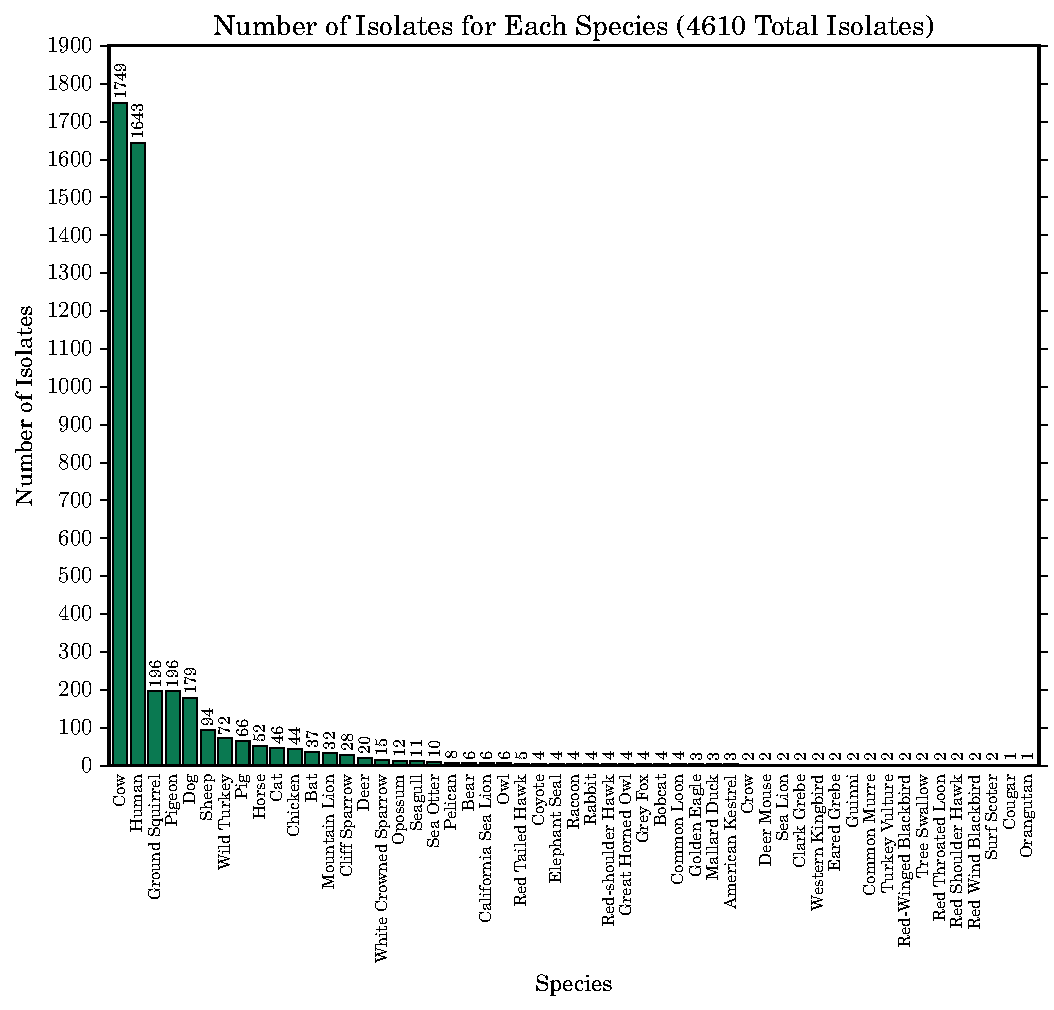
\includegraphics[height=0.85\textheight]{figures/bs/species_hist.pdf}
    %\caption{ A histogram of the number of \isols{} of each species in our study, taken from \cplop{}. There are 4,610 total \isols{} from 53 different \specs{}.}
    %\label{fig:species}
%\end{figure}
\begin{table}[]
\small
    \centering
    \begin{tabular}{|l|r|}
    \hline
    \bfseries Host Species & \bfseries Number of \Isols{} \\ \hline\hline
    Cow & 1,749 \\ \hline
    Human & 1,643 \\ \hline
    Ground Squirrel & 196 \\ \hline
    Pigeon & 196 \\ \hline
    Dog & 179 \\ \hline
    Sheep & 94 \\ \hline
    Wild Turkey & 72 \\ \hline
    Pig & 66 \\ \hline
    Horse & 52 \\ \hline
    Cat & 46 \\ \hline
    Chicken & 44 \\ \hline
    Bat & 37 \\ \hline\hline
    \textit{Other} & \textit{199} \\ \hline\hline
    \textbf{Total} & \textbf{4,610} \\ \hline
    %Mountain Lion & 32 \\ \hline
    %Cliff Sparrow & 28 \\ \hline
    %Deer & 20 \\ \hline
    %White Crowned Sparrow & 15 \\ \hline
    %Opossum & 12 \\ \hline
    %Seagull & 11 \\ \hline
    %Sea Otter & 10 \\ \hline
    %Pelican & 8 \\ \hline
    %Bear & 6 \\ \hline
    %Owl & 6 \\ \hline
    %California Sea Lion & 6 \\ \hline
    %Red Tailed Hawk & 5 \\ \hline
    %Grey Fox & 4 \\ \hline
    %Coyote & 4 \\ \hline
    %Red-shoulder Hawk & 4 \\ \hline
    %Rabbit & 4 \\ \hline
    %Elephant Seal & 4 \\ \hline
    %Bobcat & 4 \\ \hline
    %Common Loon & 4 \\ \hline
    %Great Horned Owl & 4 \\ \hline
    %Racoon & 4 \\ \hline
    %Golden Eagle & 3 \\ \hline
    %American Kestrel & 3 \\ \hline
    %Mallard Duck & 3 \\ \hline
    %Deer Mouse & 2 \\ \hline
    %Tree Swallow & 2 \\ \hline
    %Red Wind Blackbird & 2 \\ \hline
    %Eared Grebe & 2 \\ \hline
    %Crow & 2 \\ \hline
    %Clark Grebe & 2 \\ \hline
    %Red Shoulder Hawk & 2 \\ \hline
    %Surf Scoter & 2 \\ \hline
    %Red Throated Loon & 2 \\ \hline
    %Western Kingbird & 2 \\ \hline
    %Turkey Vulture & 2 \\ \hline
    %Red-Winged Blackbird & 2 \\ \hline
    %Sea Lion & 2 \\ \hline
    %Guinni & 2 \\ \hline
    %Common Murre & 2 \\ \hline
    %Cougar & 1 \\ \hline
    %Orangutan & 1 \\ \hline
    \end{tabular}
    %\caption{Caption}
    \label{tab:cplop:isolates}
\end{table}
\vfill
\end{frame}
%%%%%%%%%%%%%%%%%%%%%%%%%%%%%%%%%%%%%%%%
\begin{frame}{Empirical Work Performed Using \cplop{}}
\footnotesize
\begin{itemize}
    \item \cite{adams2016using} Using Hadoop to Identify False Positives in Bacterial Strain Typing from DNA Fingerprints 
    \item \cite{dillard2013coli} \ecoli{} Strain Demographics and Transmission in Cattle
    \item \cite{dillard2015demographics} Demographics and Transfer of \ecoli{} Within Bos taurus Populations 
    \item \textcolor<2->{cpgreen}{\cite{moritz2015application} Application of Pyroprinting for Source Tracking of E. coli in Pennington Creek}
    \item \cite{neal2012demographics} Demographics of \ecoli{} Strains in the Human Gut Using Pyroprints:  A Novel MST Method 
    \item \cite{neal2013escherichia} \ecolilong{} Strain Diversity in Humans: Effects of Sampling Effort and Methodology 
    \item \cite{nguyeninvestigating} Investigating the Dominant \ecolilong{} Strain in Lambs and Ewes Using Pyroprinting:  A Novel Method for Strain Identification
    \item \textcolor<2->{cpgreen}{\cite{shapiro2015source} Source Tracking of Fecal Contamination Along San Luis Obispo (SLO) Creek}
    \item \cite{vanderkelen2016short} Short Communication:  Typing and Tracking \textit{Bacillaceae} in Raw Milk and Milk Powder Using Pyroprinting
\end{itemize}
\end{frame}

%%%%%%%%%%%%%%%%%%%%%%%%%%%%%%%%%%%%%%%%
\section{\MSTlong{} with \cplop{}}
%%%%%%%%%%%%%%%%%%%%%%%%%%%%%%%%%%%%%%%%
\begin{frame}{\MSTlong{} with \cplop{}}{\LibDep{} \mst{}}
%\begin{block}{\MSTlong{}}
%    Any technique that aims to discover the source \spec{} of biological matter using microbiological lifeforms.
%\end{block}
\textbf{\large \LibDep{} \mst{}}

Given:
\begin{itemize}
    \item an unknown \spec{} \fib{} \isol{}
    \item a library of known \spec{} \fib{} \isols{}
\end{itemize}
Goal:
\begin{itemize}
    \item  Predict the most likely \spec{} from which the unknown \spec{} \isol{} came
\end{itemize}
\vfill
Features:
\begin{itemize}
    \item Similar to a classification technique, wherein we classify the source \spec{} of an unknown \spec{} \isol{}\footnote{also referred to as ``the unknown''}
\end{itemize}
%, given a library of known \spec{} \isols{}
\end{frame}
%%%%%%%%%%%%%%%%%%%%%%%%%%%%%%%%%%%%%%%%
\begin{frame}{\MSTlong{} with \cplop{}}{Goal \& Current Abilities}
\begin{center}
\textbf{\large Goal}

%Using a library of known \spec{} \fib{} \isols{}, predict the most likely \spec{} from which the unknown \spec{} \isol{} came
\begin{center}
\footnotesize
Unknown Species $\leftarrow$
%
Unknown Host $\leftarrow$
%
Fecal Matter $\leftarrow$
%
\Isol{} $\leftarrow$
%
\Pyro{}
\end{center}
Using \cplop{}, predict the most likely \spec{} that produced the fecal matter
\end{center}
Currently, \cplop{}:
\begin{itemize}
    \item contains \pyros{} of two \itsshort{} regions of \ecoli{} \isols{}
    \item can tell us how similar \pyros{} are
    \item can tell us which \spec{} those \isols{} came from
\end{itemize}
\end{frame}
\begin{frame}{\MSTlong{} with \cplop{}}{Our Contributions}
\textbf{Our Contributions}:
    \begin{itemize}
        \item Strain-Based \mst{} Approach Using \cplop{}
        \item \Isol{}-Based \mst{} Approach Using \cplop{}
    \end{itemize}
\end{frame}
%%%%%%%%%%%%%%%%%%%%%%%%%%%%%%%%%%%%%%%%
\subsection{Strain Typing}
%%%%%%%%%%%%%%%%%%%%%%%%%%%%%%%%%%%%%%%%
\begin{frame}{Strain Typing}
\begin{block}{Strain}
A \textit{strain} of a species of microbe is a subtype of that species where the microbes in that strain are closely related to each other in some meaningful way.
\end{block}
\begin{itemize}
    \item Microbes descending from the same parent microbe are part of the same a ``group'' or ``family''\footnote{they inherit the \dna{} of their parent}
    \item Defining strains differs between research groups
\end{itemize}
For \mst{}:
\begin{itemize}
    \item Strains of \fib{} (like \ecoli{}) tend to stay unique to the \spec{} in which they reside
\end{itemize}
In \cplop{}:
\begin{itemize}
    \item Use the similarity between \pyros{} of the two \itsshort{} regions of \ecoli{} \isols{} to define strains
\end{itemize}
\end{frame}

%%%%%%%%%%%%%%%%%%%%%%%%%%%%%%%%%%%%%%%%
% COMPARING ISOLATES
\begin{frame}{Comparing \Isols{}}
\begin{figure}
    \centering
\begin{tikzpicture}[node distance=.20in]
    \node (origin) at (0, 0) {};
    
    % Isolate A
    \node (chickenFiveOne) at (-2.25, 1) {
        \usebox\chickenFiveOne
    };
    \node[below of=chickenFiveOne]{\Ssixt{}$_A$};
    \node (chickenFiveTwo) at (-2.25, -1) {
        \usebox\chickenFiveTwo
    };
    \node[below of=chickenFiveTwo]{\Sfive{}$_A$};
    \node[above of=chickenFiveOne]{\Isol{} $A$};
    \draw[dashed] (-4,2) rectangle (-.5,-2);
    
    \visible<6->{
    \node (alpha) at (0,-3) {$\a{} = 0.995$};
    }
    
\visible<2->{
    % Isolate B
    \node (chickenSevenOne) at (2.25, 1)  {
        \usebox\chickenSevenOne
    };
    \node[below of=chickenSevenOne]{\Ssixt{}$_B$};
    \node (chickenSevenTwo) at (2.25, -1) {
        \usebox\chickenSevenTwo
    };
    \node[below of=chickenSevenTwo]{\Sfive{}$_B$};
    \node[above of=chickenSevenOne]{\Isol{} $B$};
    \draw[dashed] (4,2) rectangle (.5,-2);
}
    % Comparisons
\visible<3-4>{
    \path[<->]
            (chickenFiveOne) 
            edge[bend right] node[below, fill=white] {$\pcfunclabel(\text{\Ssixt{}}_A,\text{\Ssixt{}}_B)$} 
            (chickenSevenOne);
}
\visible<4>{
    \path[<->]
            (chickenFiveTwo) 
            edge[bend right] node[below, fill=white] {$\pcfunclabel(\text{\Sfive{}}_A,\text{\Sfive{}}_B)$} 
            (chickenSevenTwo);
}

\visible<5->{
    \path[<->]
            (chickenFiveOne) 
            edge[bend right] node[below, fill=white] {$\pcfunclabel(\text{\Ssixt{}}_A,\text{\Ssixt{}}_B) > \a{}$} 
            (chickenSevenOne);
    \path[<->]
            (chickenFiveTwo) 
            edge[bend right] node[below, fill=white] {$\pcfunclabel(\text{\Sfive{}}_A,\text{\Sfive{}}_B) > \a{}$} 
            (chickenSevenTwo);
}
\end{tikzpicture}
    \caption{Comparing \isols{} involves comparing the \pyros{} of each \isol{} using \pcfunclabel{}, the \pearson{}, with the stipulation that one can only compare \pyros{} from the same \itsshort{} in their respective \isol{}. 
    %The green bar plots represent a \pyro{} of \Ssixt{}, while gold bar plots represent a \pyro{} of \Sfive{}.
    }
    \label{fig:isolate_compare}
\end{figure}
\end{frame}

%%%%%%%%%%%%%%%%%%%%%%%%%%%%%%%%%%%%%%%%
\begin{frame}{Strain-Based}
Our strain-based \mst{} approach
\begin{enumerate}
    \item \textbf<2->{Build strains from \fib{} \isols{} in \cplop{}}
    \item Check if the unknown \isol{} belongs in a strain
    \item Classify the unknown as the most dominant \spec{} of the strain
\end{enumerate}
Relevant computer algorithms
\begin{itemize}
    \item Clustering
\end{itemize}
\visible<2->{What we focus on:}
\visible<3->{
\begin{itemize}
    \item Building strains
    \item Studying their properties
\end{itemize}
}
\end{frame}


%%%%%%%%%%%%%%%%%%%%%%%%%%%%%%%%%%%%%%%%
\section{Clustering for \BSlongs{}}
\subsection{Methodology}
%%%%%%%%%%%%%%%%%%%%%%%%%%%%%%%%%%%%%%%%
\begin{frame}{Clustering for \BSlongs{}}{\dbscan{}}

\dbscan{}:
\begin{itemize}
    \item Density-Based Clustering Algorithm
    \begin{itemize}
        \item Eric Johnson made a version for \cplop{} in \cite{johnson2015density}
    \end{itemize}
    \item Two Parameters
    \begin{itemize}
        \item \minneigh{}
        \item \eps{}
    \end{itemize}
    \item Categorizes data points as one of:
    \begin{enumerate}
        \item Core Point
        \item Border Point
        \item Noise
    \end{enumerate}
    \item Defines a cluster as:
    \begin{itemize}
        \item All Core points and their neighboring Core and Border points.
    \end{itemize}
    \item Fast as long as \compfunc{} satisfies triangle inequality\footnote{$d(x,z)\leq d(x,y) + d(y,z)$}
\end{itemize}
\end{frame}

%%%%%%%%%%%%%%%%%%%%%%%%%%%%%%%%%%%%%%%%
\begin{frame}{\dbscan{}}
%\begin{figure}
%    \centering
%    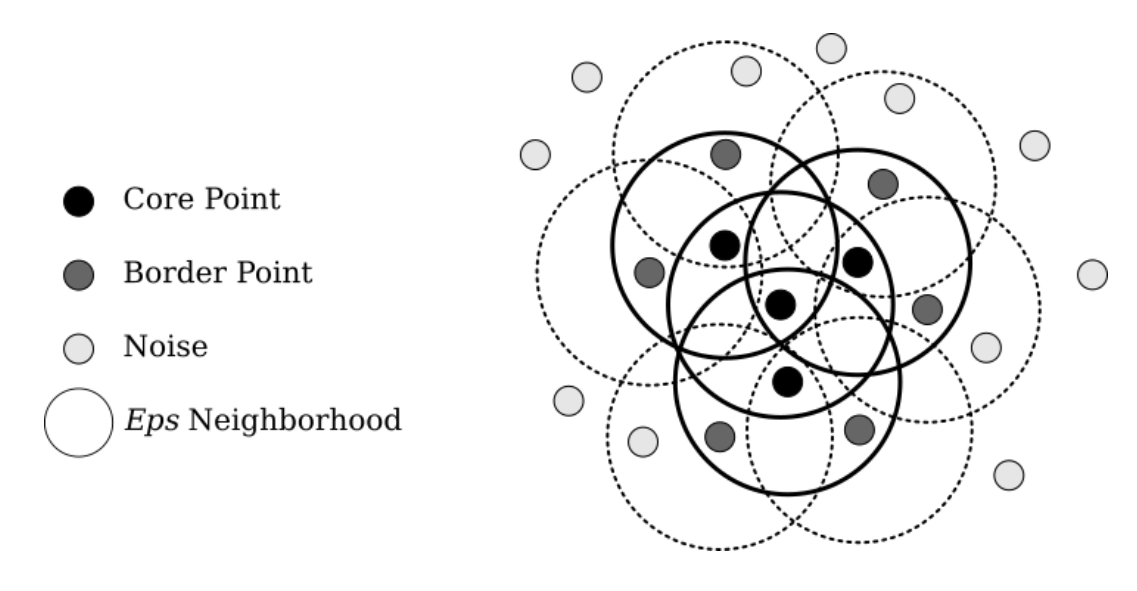
\includegraphics[width=\textwidth]{pics/dbcluster.png}
%    \caption{Example density-based cluster with \minneigh{}=3}
%    \label{fig:my_label}
%\end{figure}
% MACROS
\newcommand{\dbscanscale}{0.85}
% COLORS
\newcommand{\datacolor}{black}
\newcommand{\corecolor}{cpgreen}
\newcommand{\bordercolor}{cpgold}
\newcommand{\noisecolor}{gray}
\newcommand{\clustercolor}{cpgreengold}

% CORE
\newcommand{\datapointraw}[1]{
    \draw [fill=\datacolor] (#1) circle (.125)
}
\newcommand{\corepointraw}[1]{
    \draw [fill=\corecolor] (#1) circle (.125)
}
\newcommand{\coreneighborhood}[1]{
    \draw (#1) circle (1)
}
\newcommand{\coreneighborhoodfilled}[1]{
    \draw[fill=\clustercolor, opacity=0.50] (#1) circle (1)
}
\newcommand{\corepoint}[4]{
    \visible<#2>{\datapointraw{#1};}
    \visible<#3>{\coreneighborhood{#1};}
    \visible<#4>{\corepointraw{#1};}
}

% BORDER
\newcommand{\borderpointraw}[1]{
    \draw [fill=\bordercolor] (#1) circle (.125)
}
\newcommand{\borderneighborhood}[1]{
    \draw[dashed] (#1) circle (1)
}
\newcommand{\borderpoint}[4]{
    \visible<#2>{\datapointraw{#1};}
    \visible<#3>{\borderneighborhood{#1};}
    \visible<#4>{\borderpointraw{#1};}
}
% NOISE
\newcommand{\noisepointraw}[1]{
    \draw [fill=\noisecolor] (#1) circle (.125)
}
\newcommand{\noisepoint}[4]{
    \visible<#2>{\datapointraw{#1};}
    \visible<#3>{\borderneighborhood{#1};}
    \visible<#4>{\noisepointraw{#1};}
}
\newcommand{\coreradius}{0.80}
\newcommand{\borderradius}{1.4}
\newcommand{\noiseradiussmall}{2}
\newcommand{\noiseradiusmed}{2.85}

% FIGURE
\begin{figure}
\captionsetup[subfigure]{width=\textwidth}
\centering
%\subfloat[
%    In order to cluster using \dbscan{}, one must programmatically inspect the \eps{} neighborhood of each datapoint.
%]{
%    \begin{tikzpicture}[scale=\dbscanscale]
%        \noisepointraw{0:0};
%        \borderneighborhood{0:0};
%    \end{tikzpicture}
%}\quad
%\subfloat[
%    Categorizing datapoints as either Core Points, Border Points, or Noise is simply a matter of counting how many neighbors fall within a point's neighborhood.
%]{
    \begin{tikzpicture}[scale=\dbscanscale]
    % Core Points
    \visible<14->{\coreneighborhoodfilled{0:0};}
    \visible<14->{\coreneighborhoodfilled{0:\coreradius};}
    \visible<14->{\coreneighborhoodfilled{120:\coreradius};}
    \visible<14->{\coreneighborhoodfilled{240:\coreradius};}
    \corepoint{0  :0          }{-2}{2-9,13-}{3-}
    \corepoint{0  :\coreradius}{-4}{4-9,13-}{5-}
    \corepoint{120:\coreradius}{-4}{4-9,13-}{5-}
    \corepoint{240:\coreradius}{-4}{4-9,13-}{5-}
    
    % Border Points1
    \borderpoint{ 90:\borderradius}{-6}{6-9}{7-}
    \borderpoint{150:\borderradius}{-8}{8-9}{9-}
    \borderpoint{210:\borderradius}{-8}{8-9}{9-}
    \borderpoint{270:\borderradius}{-8}{8-9}{9-}
    \borderpoint{ 30:\borderradius}{-8}{8-9}{9-}
    \borderpoint{330:\borderradius}{-8}{8-9}{9-}
    
    % Noise Points
    \noisepoint{ 20:\noiseradiussmall}{-11}{11-12}{12-}
    \noisepoint{ 90:\noiseradiussmall}{-11}{11-12}{12-}
    \noisepoint{  0:\noiseradiusmed  }{-11}{11-12}{12-}
    \noisepoint{180:\noiseradiusmed  }{-11}{11-12}{12-}
    \noisepoint{ 60:\noiseradiusmed  }{-11}{11-12}{12-}
    \noisepoint{120:\noiseradiusmed  }{-11}{11-12}{12-}
    \noisepoint{300:\noiseradiusmed  }{-11}{11-12}{12-}
    \noisepoint{240:\noiseradiusmed  }{-11}{11-12}{12-}
    \noisepoint{220:\noiseradiussmall}{-11}{11-12}{12-}
    \noisepoint{260:\noiseradiussmall}{-11}{11-12}{12-}
    \noisepoint{340:\noiseradiussmall}{-11}{11-12}{12-}
    \end{tikzpicture}
    %\vspace{12pt}
    \hfill
    \begin{tikzpicture}[scale = \dbscanscale]
    \datapointraw{0:0}       node[anchor=west, xshift=4pt] {Data Point};
    \corepointraw{270:.4}      node[anchor=west, xshift=4pt] {Core Point};
    \borderpointraw{270:.8}  node[anchor=west, xshift=4pt] {Border Point};
    \noisepointraw{270:1.2}  node[anchor=west, xshift=4pt] {Noise};
    \draw[dashed] (270:1.6) circle (0.125) node[anchor=west, xshift=4pt] {\eps{}-Neighborhood};
    \end{tikzpicture}
%}
\caption{A basic density-based clustering with \minneigh{} = 3 points.
%represented by the circles --- solid for the core neighborhoods and dashed for border (recreated from \cite{johnson2015density}).
%We see that the green points each contain 3 neighbors, but while the border points do not, they are within \eps{} of a core point and we thus cluster it along with the core points.
%The (single) cluster that results from this set of datapoints are the green and gold points depicted.
}
\label{fig:density-based-clustering}
\end{figure}
\end{frame}

%%%%%%%%%%%%%%%%%%%%%%%%%%%%%%%%%%%%%%%%%
\begin{frame}{DBSCAN}{Distance Metric Satisfying Triangle Inequality}
\[
    \pcfunc{\pca{}}{\pcb{}}
    =
    %\pclong{\pcveca}{\pcvecb}
    \pceric{\pca{}}{\pcb{}}
    =
    \frac{\veccov{\pca{}}{\pcb{}}}{\vecstddev{\pca{}}\cdot\vecstddev{\pcb}}
    %\frac{cov(\vec{u},\vec{p})}{\sigma_{\vec{u}}\cdot %\sigma_{\vec{p}}} 
\]
The \zscore{} of \pcveca{} is:
\[
\zscoreeq{\pca}
\]
Distance Metric:
\[
\eucz{\pca}{\pcb}
\]
\[
\euczalternate{\pca}{\pcb}
\]
\end{frame}

%%%%%%%%%%%%%%%%%%%%%%%%%%%%%%%%%%%%%%%%%
\begin{frame}{DBSCAN}{Converted $\alpha$ Threshold as \eps{} for Range Querying}
\begin{table}[]
\centering
\caption{Converted $\alpha$ threshold used for \eps{} to fit the new metric space, where \numdims{} is the number of nucleotide dispensations for that \itsshort{}'s \pyro{}.}
\label{tab:converted_thresholds}
\begin{tabular}{|c|c|c|}
\hline
\textbf{\itsshort{} Region} & \Ssixt{}     & \Sfive{}     \\
                            & $\alpha$     & $\alpha$     \\ \hline
\pcfunc{\pca}{\pcb}         & 0.995        & 0.995        \\ \hline
\numdims{}                  & \Ssixtdims{} & \Sfivedims{} \\ \hline
\euczfunc{\pca{}}{\pcb{}}   & 0.9747       & 0.9644       \\ \hline
\end{tabular}
\end{table}
\vfill
\eps{} Range Query:
\begin{itemize}
    \item Returns neighbor \isols{} are within \a{} in \textbf{both} \itsshort{} regions
\end{itemize}
\end{frame}

%%%%%%%%%%%%%%%%%%%%%%%%%%%%%%%%%%%%%%%%
\subsection{Evaluation}
%%%%%%%%%%%%%%%%%%%%%%%%%%%%%%%%%%%%%%%%
\begin{frame}{Evaluation Metrics}
Clustering for \mst{} procedure:
\begin{enumerate}
    \item Build strains (clusters) from \isols{} in \cplop{} (using \dbscan{})
    \item Check if the unknown \isol{} belongs in a strain (cluster)
    \item Classify the unknown as the most dominant \spec{} of the strain (cluster)
\end{enumerate}

Two Outcomes:
\begin{itemize}
    \item \Isol{} is part of a strain (cluster)
    \item \Isol{} is not part of a strain (categorized as noise)
\end{itemize}

Evaluation Metrics:
\begin{itemize}
    \item Individual Cluster Purity
    \item Overall Clustering Purity
    \item Clustering Coverage
\end{itemize}
\end{frame}
%%%%%%%%%%%%%%%%%%%%%%%%%%%%%%%%%%%%%%%%
\newcommand{\slice}[4]{
  \pgfmathparse{0.5*#1+0.5*#2}
  \let\midangle\pgfmathresult

  % slice
  \draw[thick,fill=cpgold!40] (0,0) -- (#1:1) arc (#1:#2:1) -- cycle;

  % outer label
  \node[label=\midangle:#4] at (\midangle:1) {};

  % inner label
  \pgfmathparse{min((#2-#1-10)/110*(-0.3),0)}
  \let\temp\pgfmathresult
  \pgfmathparse{max(\temp,-0.5) + 0.8}
  \let\innerpos\pgfmathresult
  \node at (\midangle:\innerpos) {#3};
}

\begin{frame}[fragile]{Individual Cluster Purity}
\small
Consider a cluster $C=\{c_1,\ldots, c_K\}$. Let $s(c)$ refer to the species of isolate $c$.
Let $m$ be the most dominant species label for data points in $C$, and let the total number of points in
$C$ with $s(c) = m$ be $s_m$. Then the \textit{individual cluster purity} $\nu$ of cluster $C$ is:

\[
    \nu(C) = \frac{s_m}{K}
\]
\begin{center}
\begin{tikzpicture}[scale=1.75]
\newcounter{a}
\newcounter{b}
\foreach \p/\t in {47/Dog,38/Chicken,15/Pigeon}
  {
    \setcounter{a}{\value{b}}
    \addtocounter{b}{\p}
    \slice{\thea/100*360}
          {\theb/100*360}
          {\p\%}{\t}
  }

\end{tikzpicture}
\end{center}
\end{frame}

%%%%%%%%%%%%%%%%%%%%%%%%%%%%%%%%%%%%%%%%
\begin{frame}{Overall Clustering Purity}
Given a \textit{clustering} $\mathcal{C} = \{C_1,\dots,C_n\}$ on a dataset, we define the size $\mathcal{M}$ of the set of clusters: 
\[
    \mathcal{M} = \sum_{i = 0}^{n} |C_i|
\]
The \textit{overall clustering purity} is:
\[
    \sum_{i=1}^{n} \frac{|C_i|}{\mathcal{M}}\cdot\nu(C_i)
\]
\end{frame}

%%%%%%%%%%%%%%%%%%%%%%%%%%%%%%%%%%%%%%%%
\begin{frame}{Components Clustering Coverage}
Number of \isols{} in:
\begin{enumerate}
    \item A noise/outlier point
    \item A  \textit{100\% pure} cluster
    \item A cluster where its \spec{} is the most dominant
    \item A cluster where its \spec{} is in minority
\end{enumerate} 
\end{frame}
%%%%%%%%%%%%%%%%%%%%%%%%%%%%%%%%%%%%%%%%
\subsection{Results}
%%%%%%%%%%%%%%%%%%%%%%%%%%%%%%%%%%%%%%%%
%%%%%%%%%%%%%%%%%%%%%%%%%%%%%%%%%%%%%%%%
% SIZE DSTRIBUTION
\begin{frame}{Size Distribution}{\minneigh{} = 3}
    \centering
    \begin{figure}
    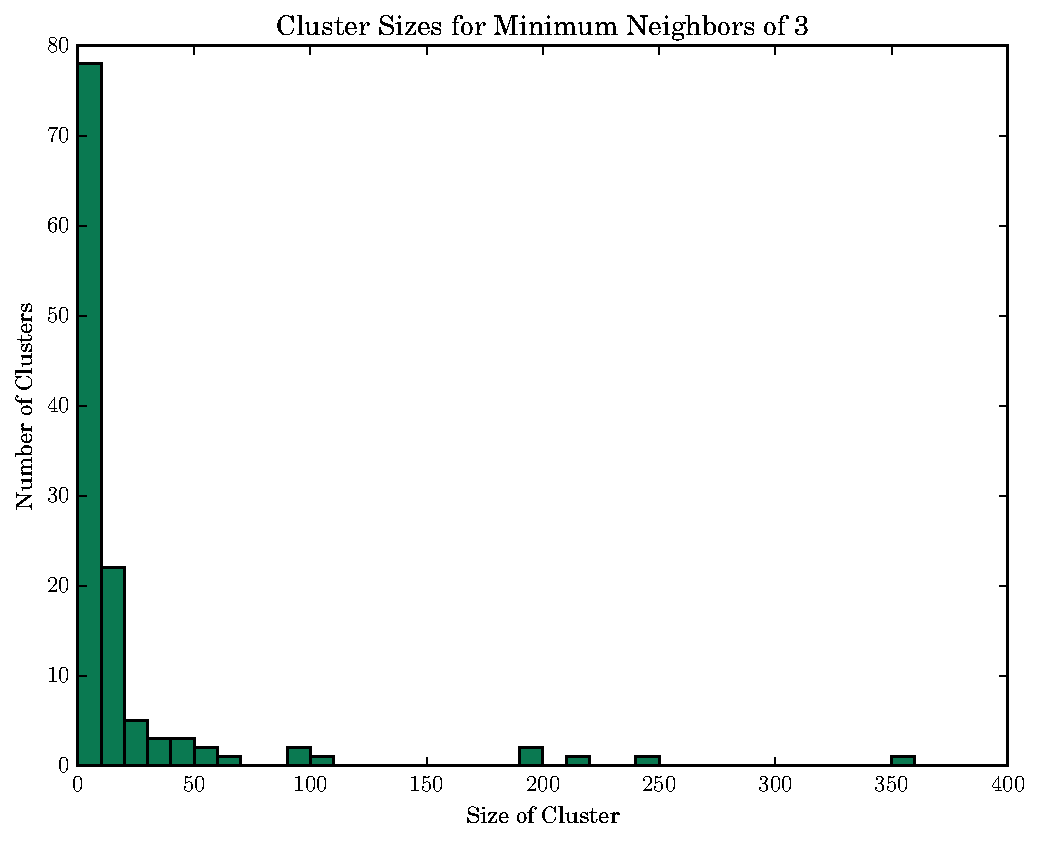
\includegraphics[width=0.85\linewidth]{figures/bs/neigh_size_3}
    %\caption{Cluster Size Distribution for \minneigh{} of 3} 
    \label{fig:big:clust_size_dist_3}
    \end{figure}
\end{frame}
    
\begin{frame}{Size Distribution}{\minneigh{} = 5}
    \centering
    \begin{figure}
    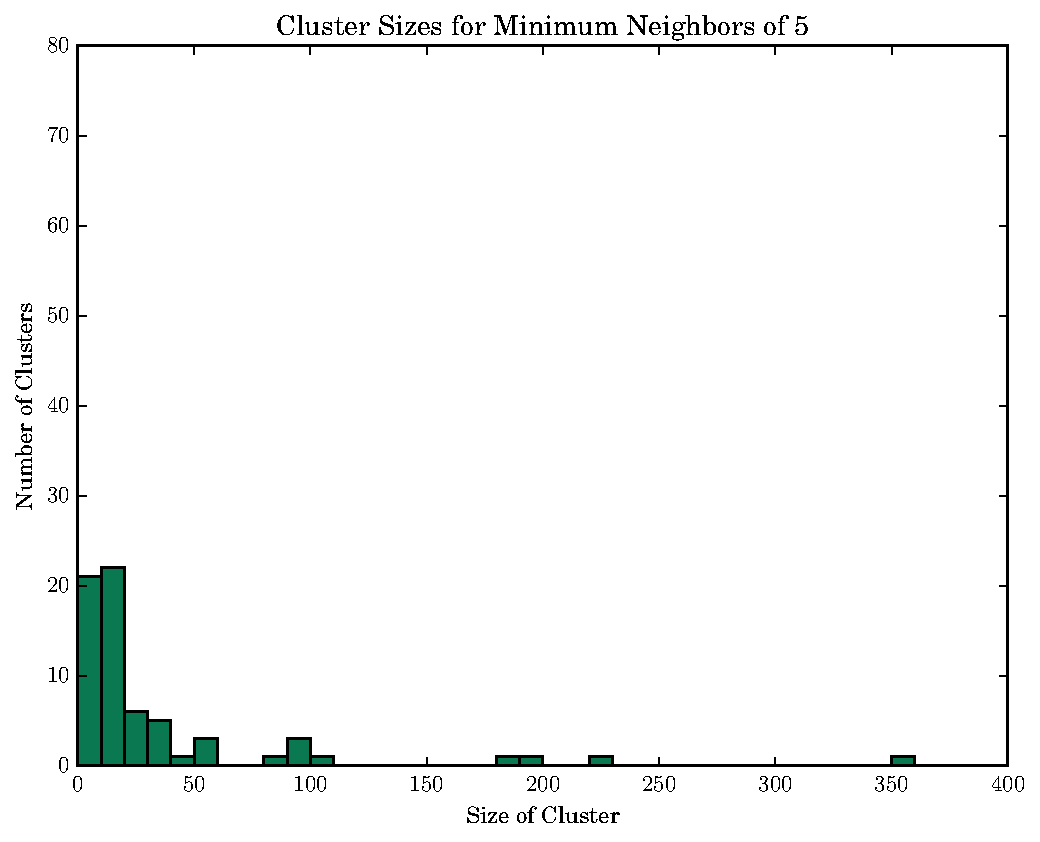
\includegraphics[width=0.85\linewidth]{figures/bs/neigh_size_5}
    %\caption{Cluster Size Distribution for \minneigh{} of 5} 
    \label{fig:big:clust_size_dist_5}
    \end{figure}
\end{frame}
    
\begin{frame}{Size Distribution}{\minneigh{} = 7}
    \centering
    \begin{figure}
    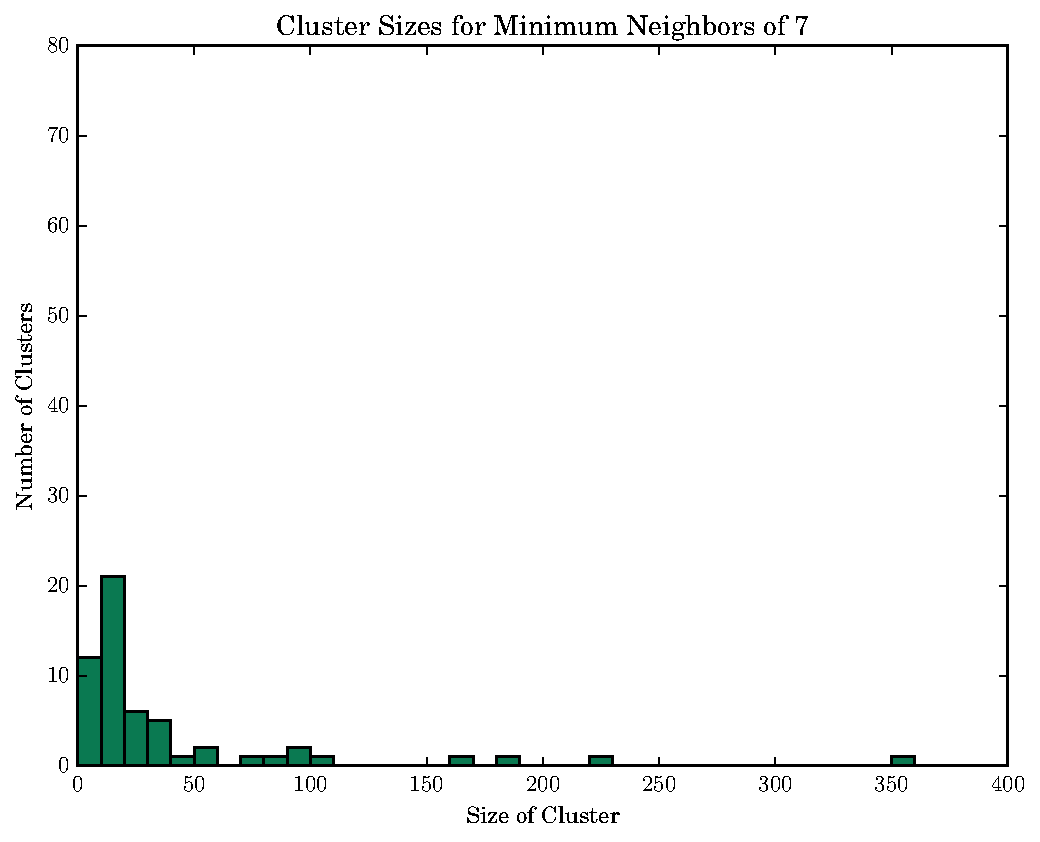
\includegraphics[width=0.85\linewidth]{figures/bs/neigh_size_7}
    %\caption{Cluster Size Distribution for \minneigh{} of 7} 
    \label{fig:big:clust_size_dist_7}
    \end{figure}
\end{frame}
%%%%%%%%%%%%%%%%%%%%%%%%%%%%%%%%%%%%%%%%
% SIZE DSTRIBUTION
\begin{frame}{Size Distribution}
\begin{figure}[ht!]
    \centering
    \begin{subfigure}{0.30\textwidth}
    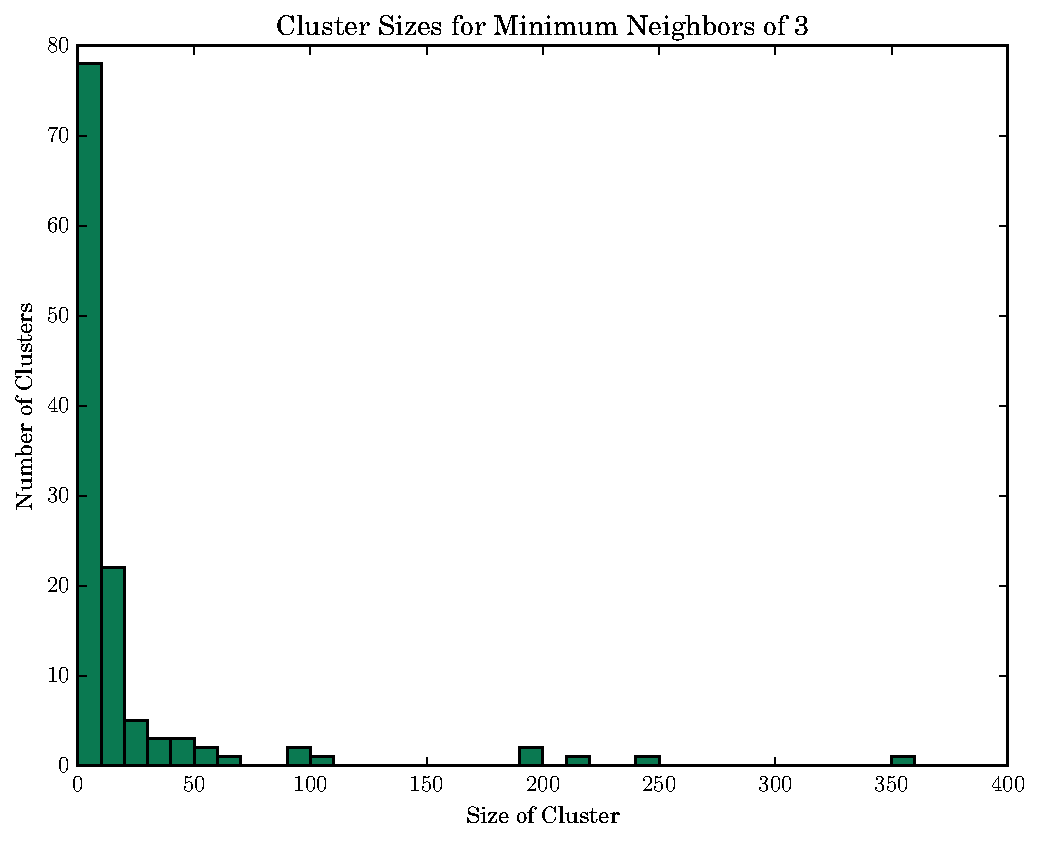
\includegraphics[width=\linewidth]{figures/bs/neigh_size_3}
    %\caption{Cluster Size Distribution for \minneigh{} of 3} 
    \label{fig:clust_size_dist_3}
    \end{subfigure}
    \centering
    \begin{subfigure}{0.30\textwidth}
    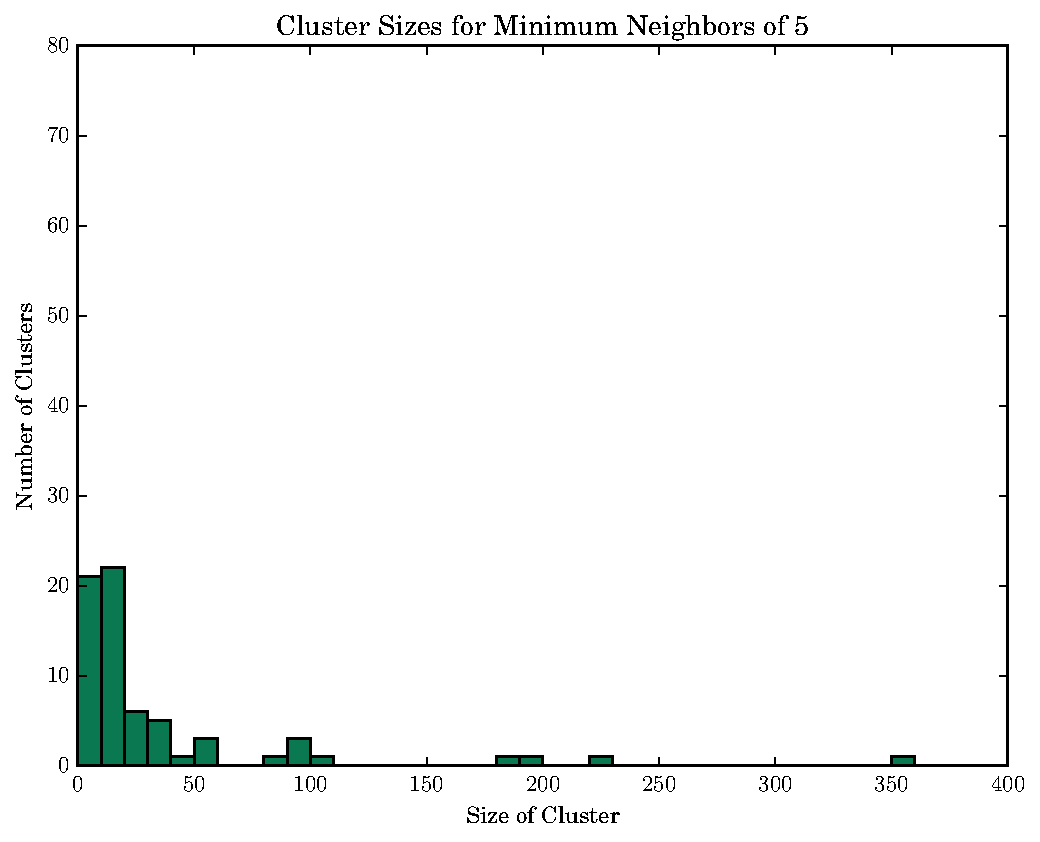
\includegraphics[width=\linewidth]{figures/bs/neigh_size_5}
    %\caption{Cluster Size Distribution for \minneigh{} of 5} 
    \label{fig:clust_size_dist_5}
    \end{subfigure}
    \centering
    \begin{subfigure}{0.30\textwidth}
    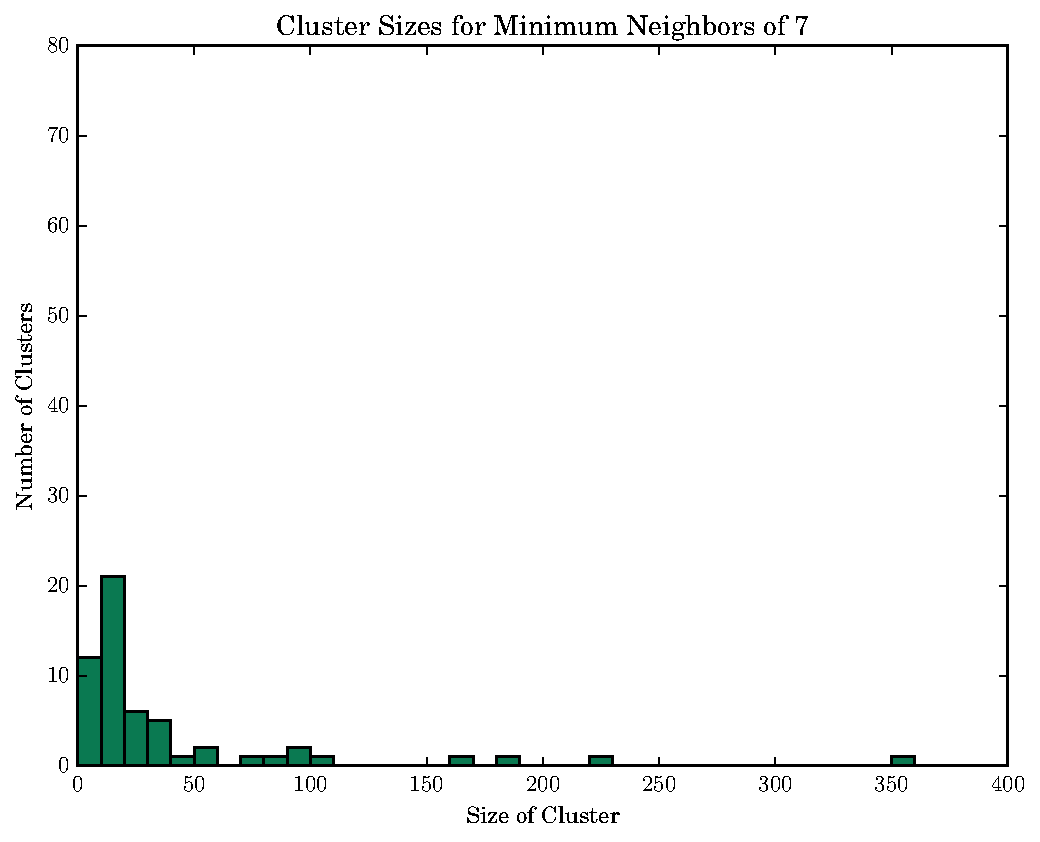
\includegraphics[width=\linewidth]{figures/bs/neigh_size_7}
    %\caption{Cluster Size Distribution for \minneigh{} of 7} 
    \label{fig:clust_size_dist_7}
    \end{subfigure}
    %\caption{The size distribution of clusters skews heavily towards smaller clusters.}
    \label{fig:clust_size_dist}
\end{figure}
\end{frame}

%%%%%%%%%%%%%%%%%%%%%%%%%%%%%%%%%%%%%%%%
\begin{frame}{Individual Cluster Purity}{\minneigh{} = 3}
    \centering
    \begin{figure}
    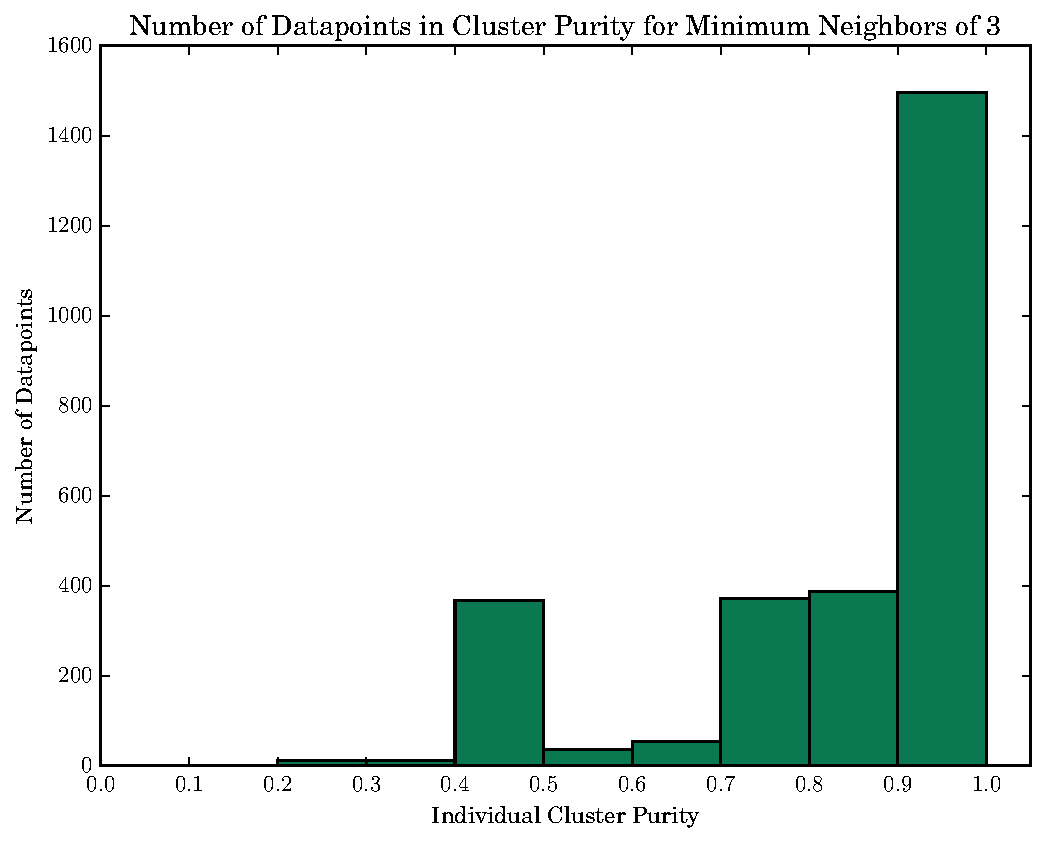
\includegraphics[width=0.85\linewidth]{figures/bs/neigh_dist_data_3}
    %\caption{Individual Clsuter Purity Distribution for \minneigh{} of 3} 
    \label{fig:clust_purity_ind_3}
    \end{figure}
\end{frame}
\begin{frame}{Individual Cluster Purity}{\minneigh{} = 5}
    \centering
    \begin{figure}
    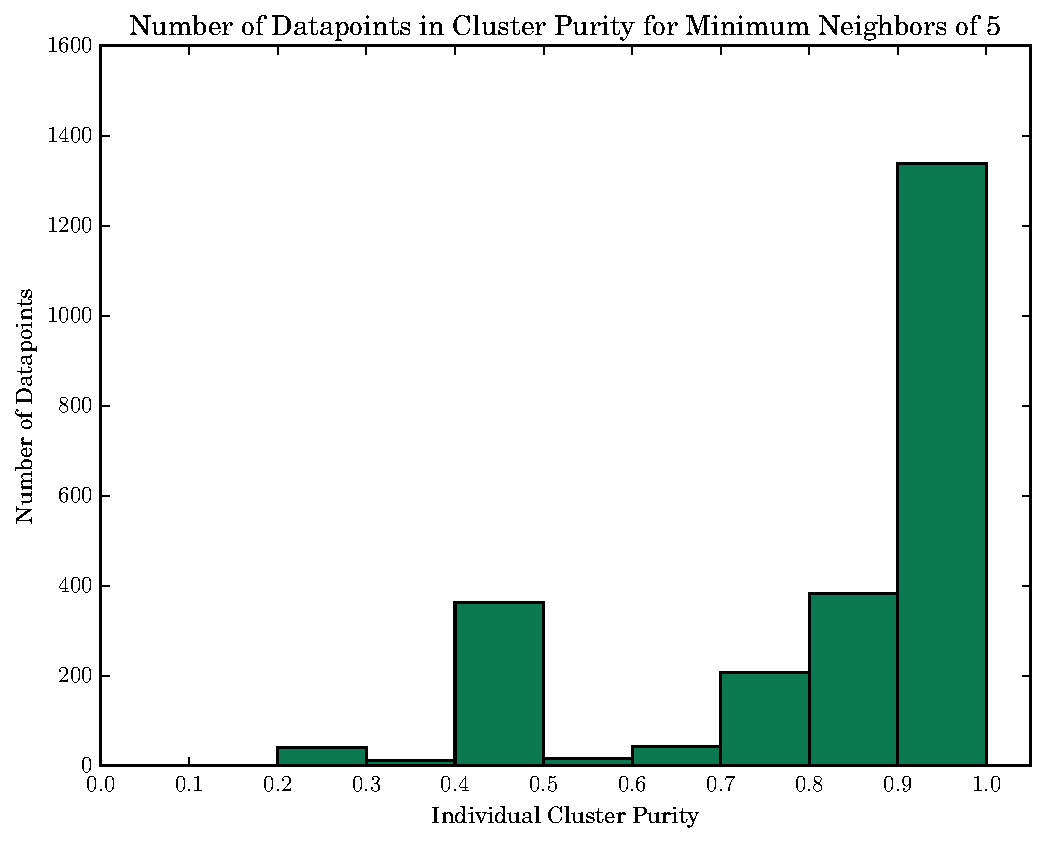
\includegraphics[width=0.85\linewidth]{figures/bs/neigh_dist_data_5}
    \label{fig:clust_purity_ind_5}
    \end{figure}
\end{frame}
\begin{frame}{Individual Cluster Purity}{\minneigh{} = 7}
    \centering
    \begin{figure}
    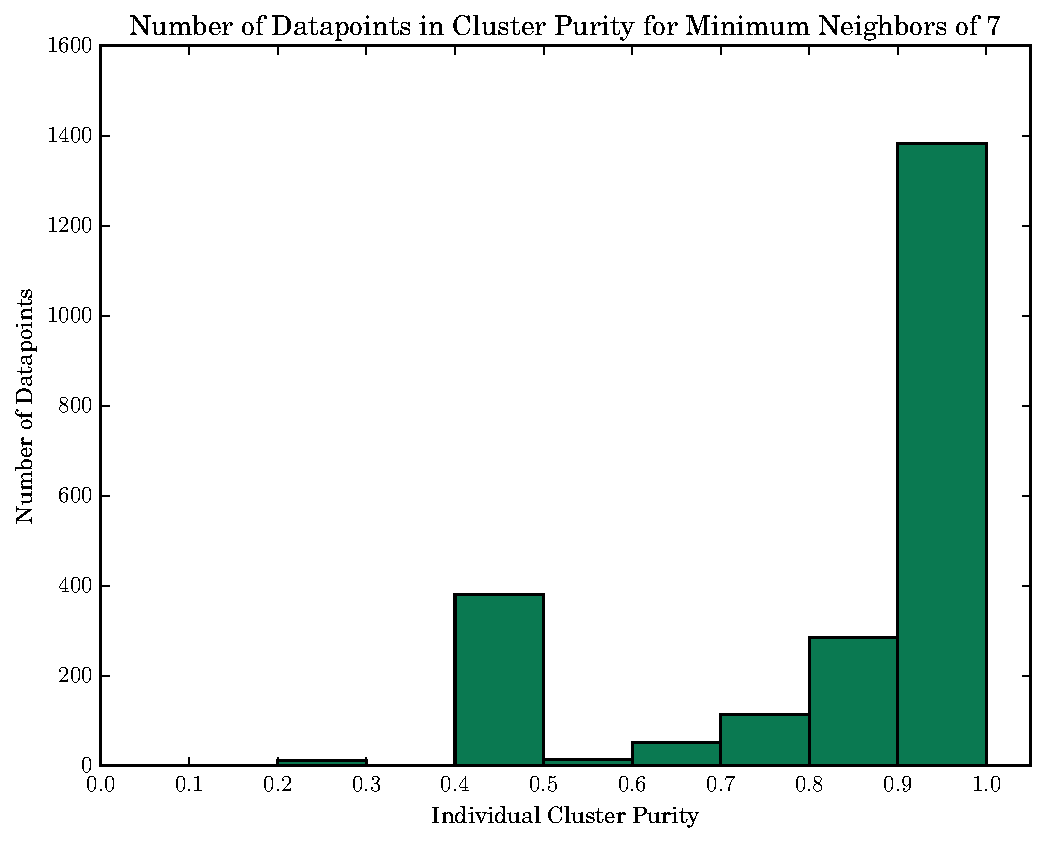
\includegraphics[width=0.85\linewidth]{figures/bs/neigh_dist_data_7}
    \label{fig:clust_purity_ind_7}
    \end{figure}
    \label{fig:clust_purity_ind}
\end{frame}


%%%%%%%%%%%%%%%%%%%%%%%%%%%%%%%%%%%%%%%%
\begin{frame}{Individual Cluster Purity}
\begin{figure}[ht!]
    \centering
    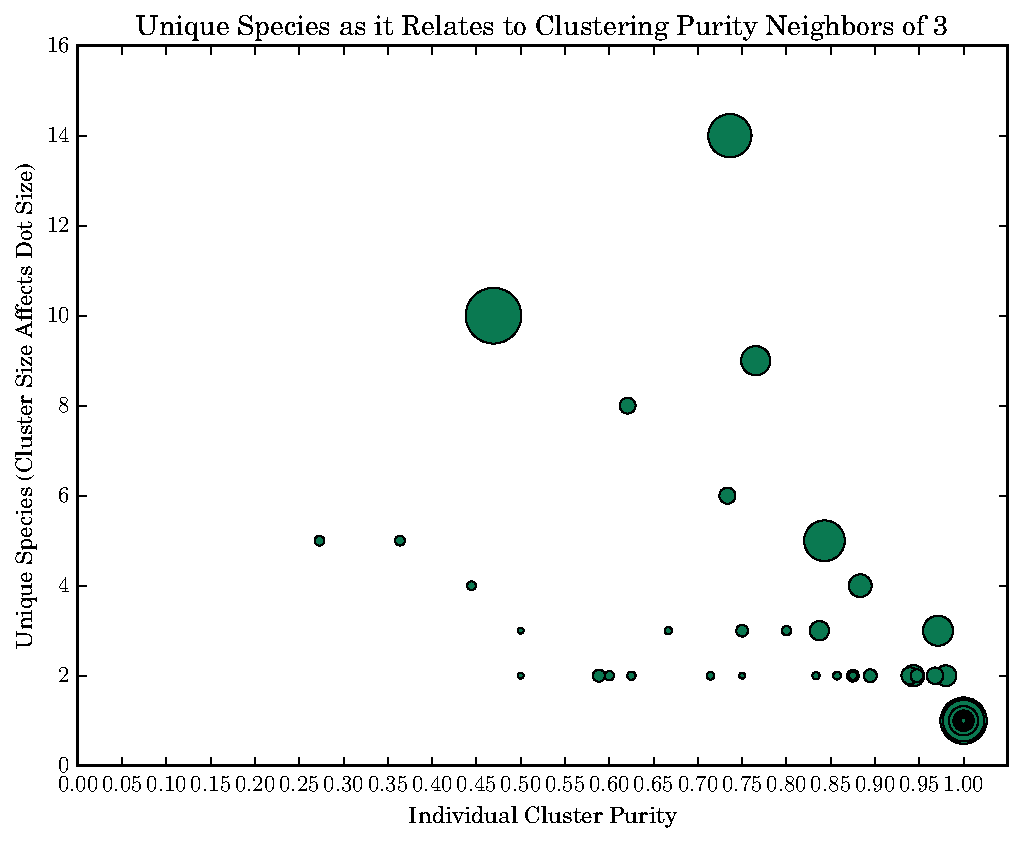
\includegraphics[width=0.85\linewidth]{figures/bs/neigh_purity_unique_3_size}
    \label{fig:clustered:3}
\end{figure}
\begin{tikzpicture}[remember picture,overlay, shift={(current page.center)}]
\pause
  \visible<+->{
    \node[]   (purepoints) at (5cm,0)  {$1,206$};
    \path[->] (purepoints) edge [bend left, line width=1pt] (4.35cm,-2.5cm);
  }
  \visible<+>{
      \draw[] (2.90cm,-2.30cm) ellipse (1.25cm and 0.25cm);
  }
  \visible<+>{
      \draw[rotate around={-35:(-0.75cm,-1.65cm)}] (-0.75cm,-1.65cm) ellipse (1.35cm and 0.5cm);
  }
  \visible<+>{
    \path[->] (5cm,2cm) edge [bend right, line width=1pt] (0.15cm,1.15cm);
  }
  \visible<+>{
    \path[->] (5cm,2cm) edge [bend right, line width=1pt] (2.25cm,2.75cm);
  }
\end{tikzpicture}
\end{frame}

%%%%%%%%%%%%%%%%%%%%%%%%%%%%%%%%%%%%%%%%
\begin{frame}{Individual Cluster Purity}
\begin{figure}[ht!]
    \centering
    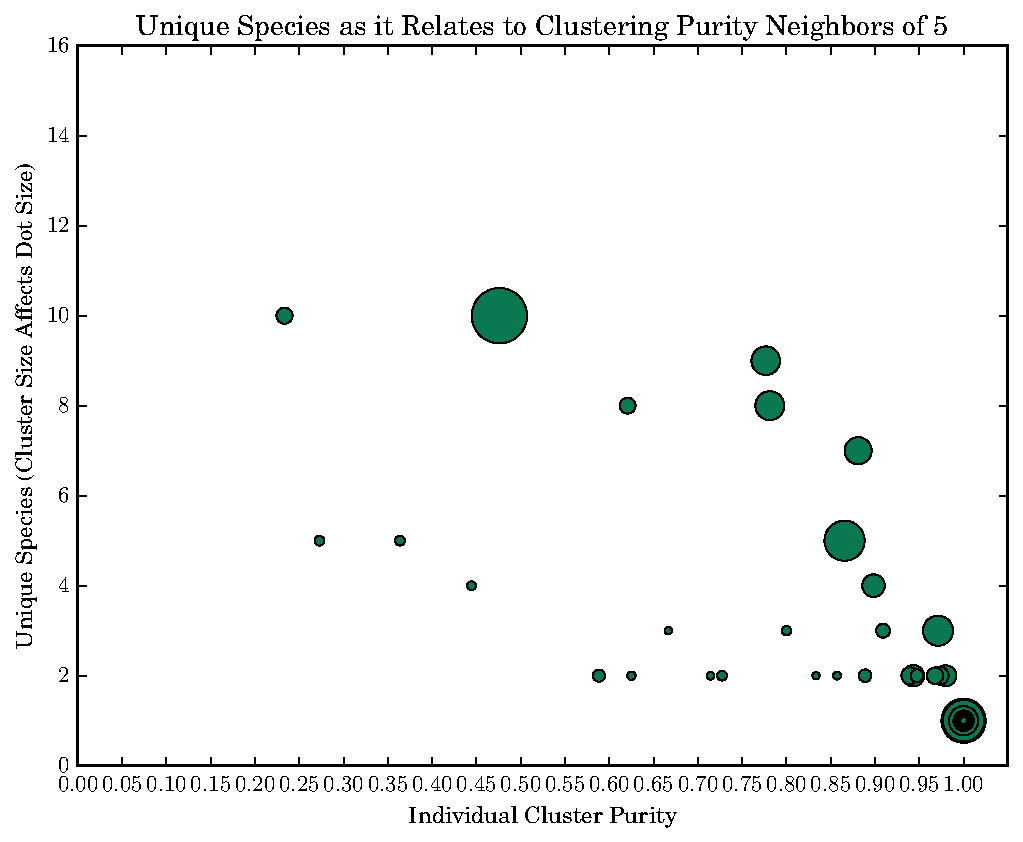
\includegraphics[width=0.85\linewidth]{figures/bs/neigh_purity_unique_5_size}
    \label{fig:clustered:5}
\end{figure}
\begin{tikzpicture}[remember picture,overlay, shift={(current page.center)}]
    \node[]   (purepoints) at (5cm,0)  {$990$};
    \path[->] (purepoints) edge [bend left, line width=1pt] (4.35cm,-2.5cm);
    \path[->] (5cm,2cm) edge [bend right, line width=1pt] (2.50cm,0.30cm);
    \path[->] (5cm,2cm) edge [bend right, line width=1pt] (3.15cm,0.0cm);
\end{tikzpicture}
\end{frame}

%%%%%%%%%%%%%%%%%%%%%%%%%%%%%%%%%%%%%%%%
\begin{frame}{Individual Cluster Purity}
\begin{figure}[ht!]
    \centering
    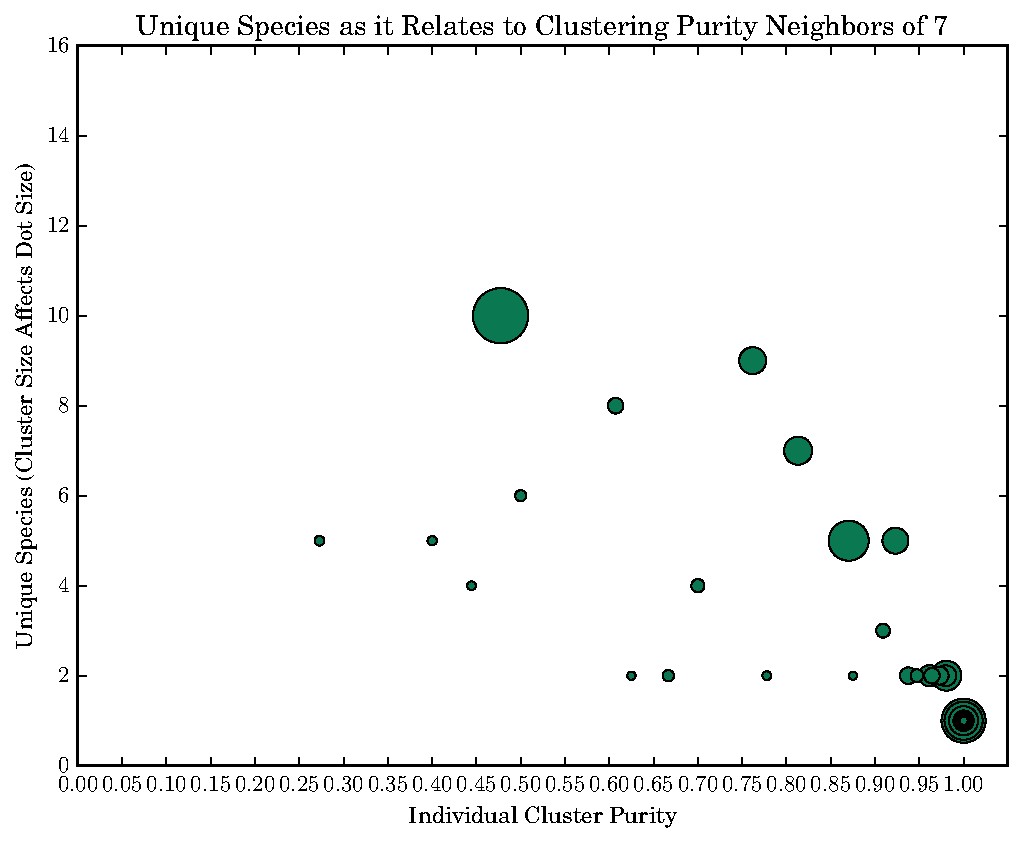
\includegraphics[width=0.85\linewidth]{figures/bs/neigh_purity_unique_7_size}
    \label{fig:clustered:7}
\end{figure}
\begin{tikzpicture}[remember picture,overlay, shift={(current page.center)}]
    \node[]   (purepoints) at (5cm,0)  {$962$};
    \path[->] (purepoints) edge [bend left, line width=1pt] (4.35cm,-2.5cm);
\end{tikzpicture}
\end{frame}

%%%%%%%%%%%%%%%%%%%%%%%%%%%%%%%%%%%%%%%%
\begin{frame}{Individual Cluster Purity}
\begin{figure}[ht!]
    \centering
    \begin{subfigure}{0.30\textwidth}
    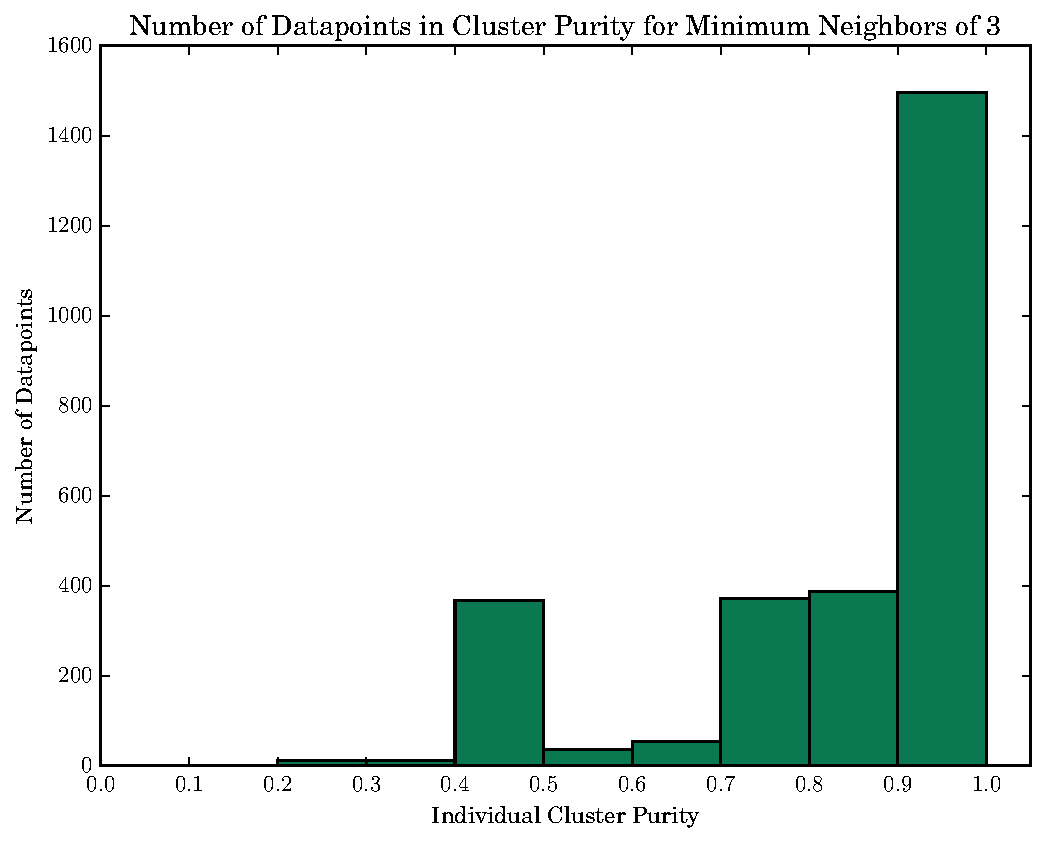
\includegraphics[width=\linewidth]{figures/bs/neigh_dist_data_3}
    \label{fig:clust_purity_dist_3}
    \end{subfigure}
    \centering
    \begin{subfigure}{0.30\textwidth}
    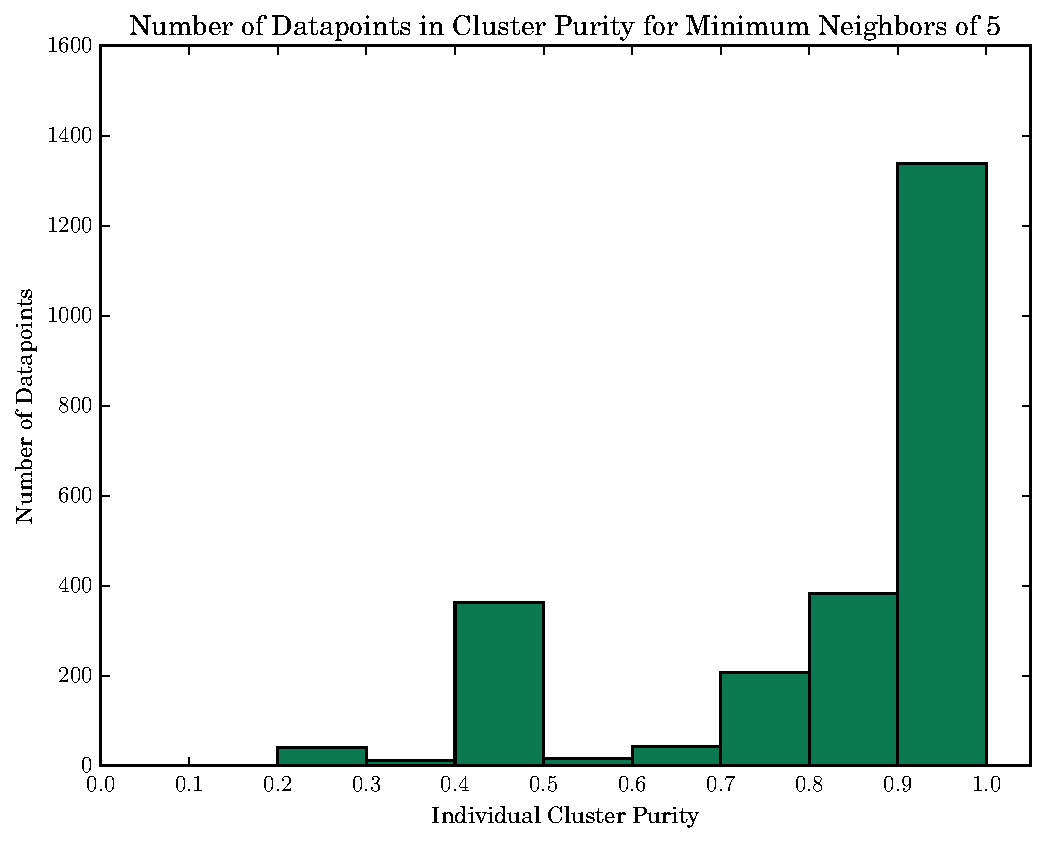
\includegraphics[width=\linewidth]{figures/bs/neigh_dist_data_5}
    \label{fig:clust_purity_dist_5}
    \end{subfigure}
    \centering
    \begin{subfigure}{0.30\textwidth}
    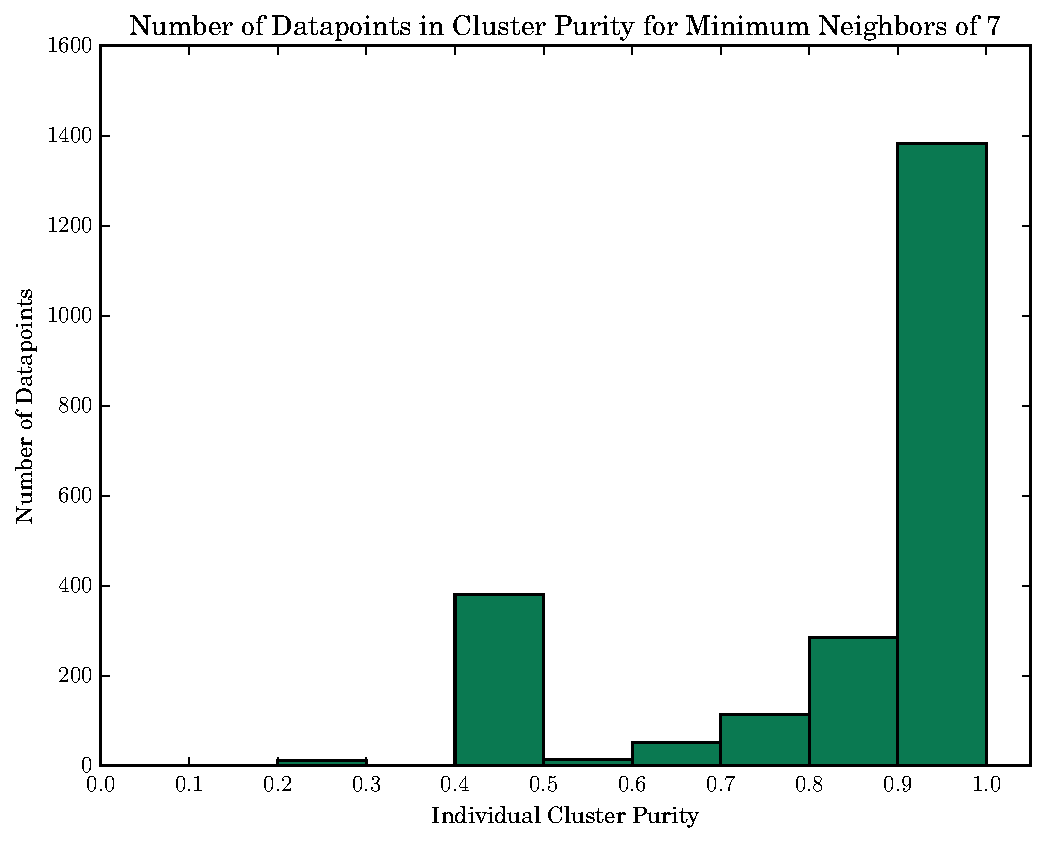
\includegraphics[width=\linewidth]{figures/bs/neigh_dist_data_7}
    \label{fig:clust_purity_dist_7}
    \end{subfigure}
    \label{fig:clust_purity_dist}
\end{figure}

\begin{figure}[ht!]
    \centering
    \begin{subfigure}{0.30\textwidth}
    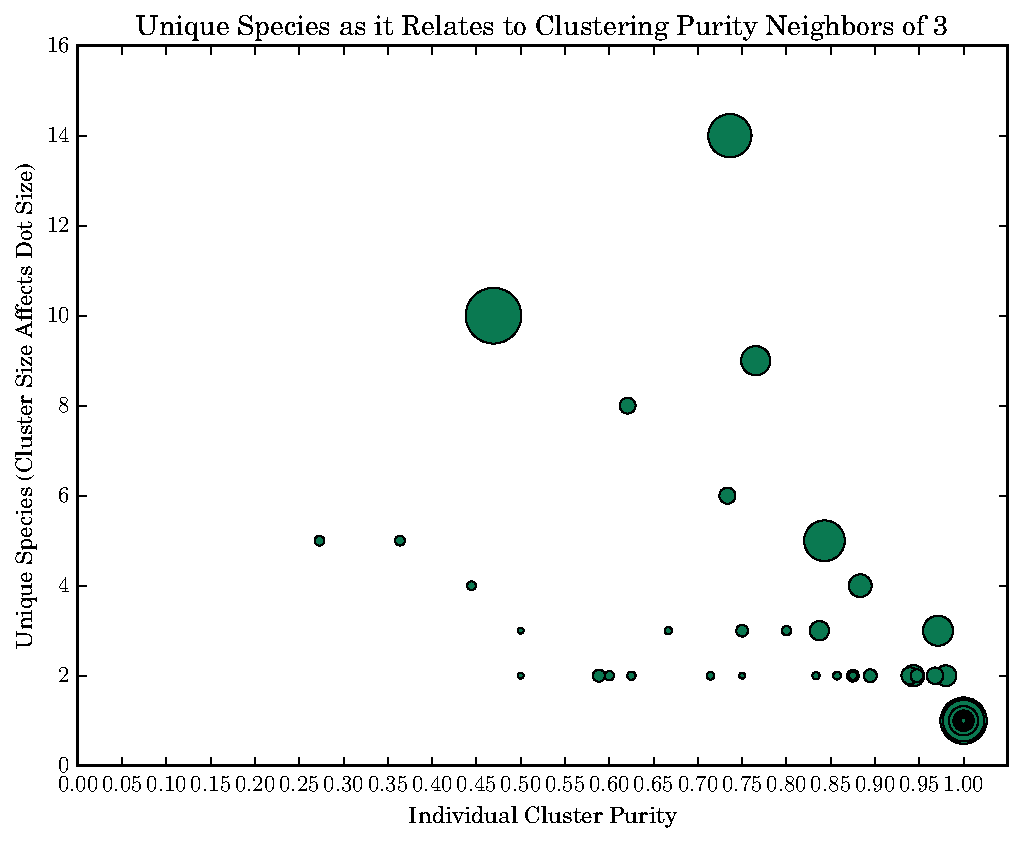
\includegraphics[width=\linewidth]{figures/bs/neigh_purity_unique_3_size}
    \label{fig:clust_pure_3}
    \end{subfigure}
    \centering
    \begin{subfigure}{0.30\textwidth}
    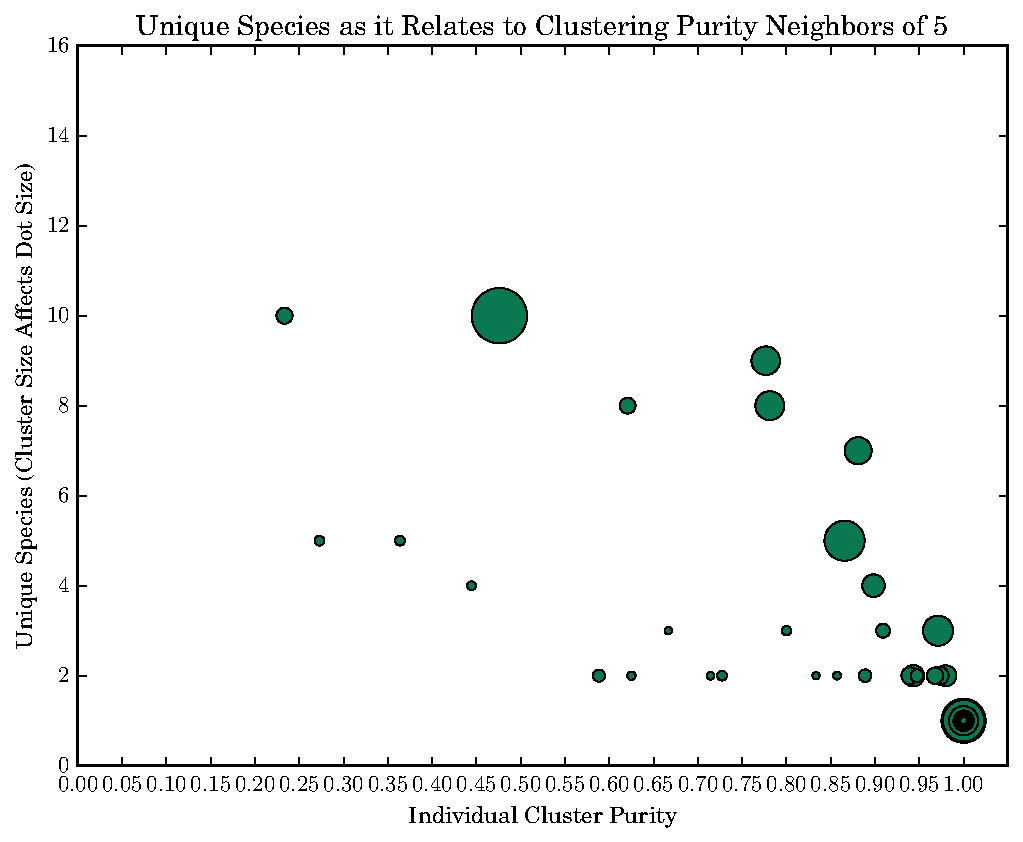
\includegraphics[width=\linewidth]{figures/bs/neigh_purity_unique_5_size}
    \label{fig:clust_pure_5}
    \end{subfigure}
    \centering
    \begin{subfigure}{0.30\textwidth}
    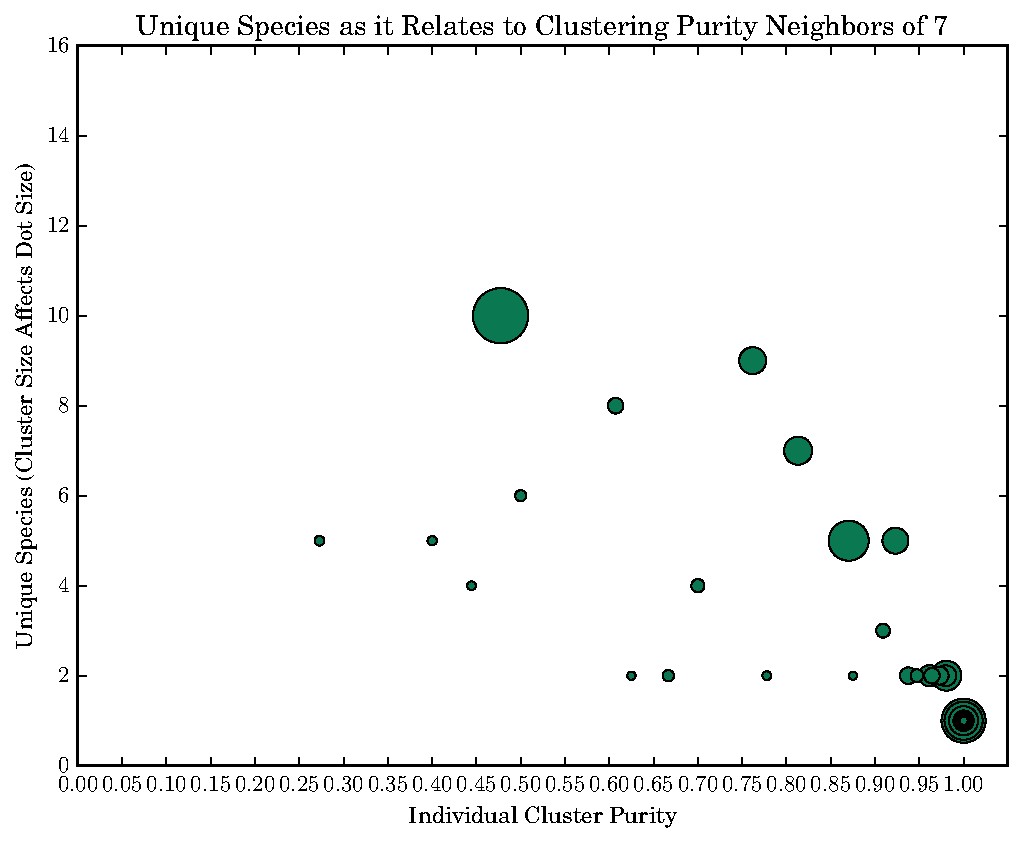
\includegraphics[width=\linewidth]{figures/bs/neigh_purity_unique_7_size}
    \label{fig:clust_pure_7}
    \end{subfigure}
    \label{fig:clust_pure}
\end{figure}
\end{frame}

%%%%%%%%%%%%%%%%%%%%%%%%%%%%%%%%%%%%%%%%
\begin{frame}{Clustering Coverage}
\begin{figure}[ht!]
    \centering
    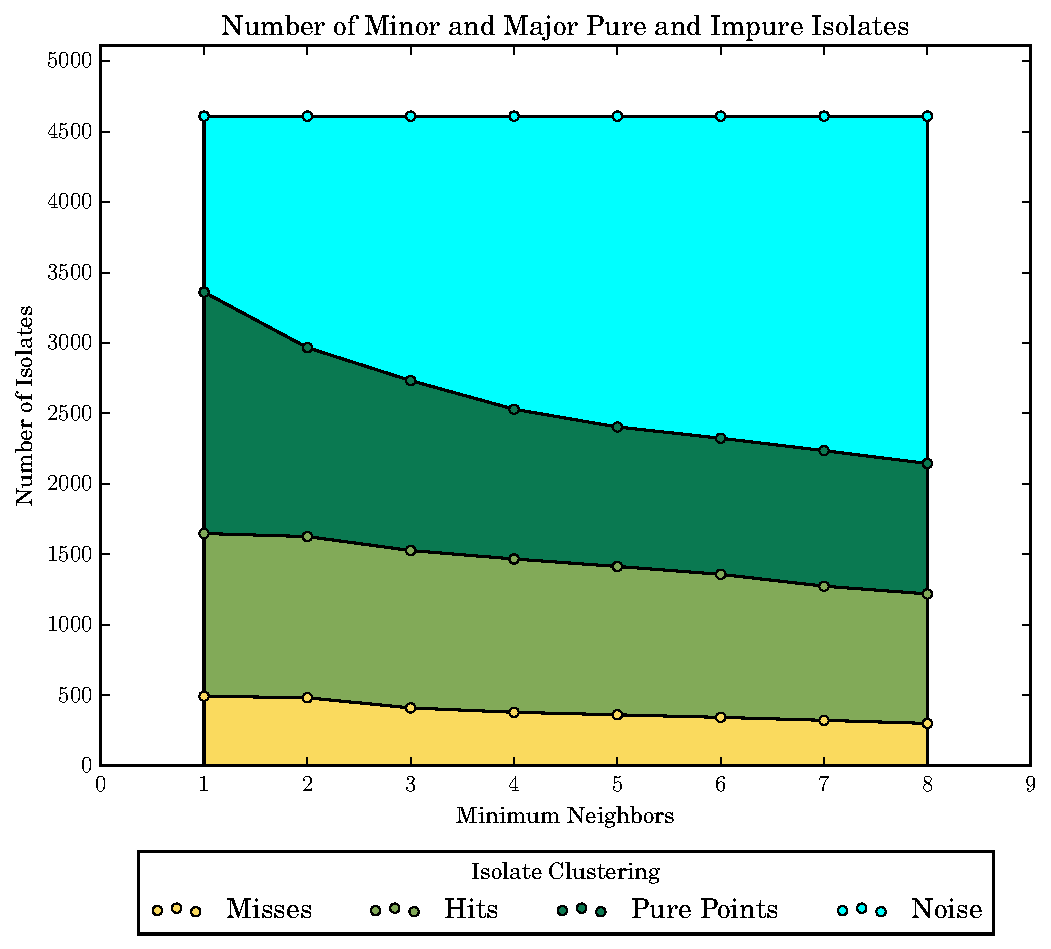
\includegraphics[width=0.75\linewidth]{figures/bs/neigh_minor_major_impure_filled_stack}
    %\caption{As \minneigh{} increases, we see that we cluster fewer \isols{}. throughout, the number of major pure \isols{} stays relatively equal to the number of major impure \isols{}.}
    \label{fig:clustered}
\end{figure}
\end{frame}

%%%%%%%%%%%%%%%%%%%%%%%%%%%%%%%%%%%%%%%%
\begin{frame}{Overall Clustering Purity vs. \mst{} Accuracy}{Includes Unclustered (Unclassified)}
\begin{figure}[ht!]
    \centering
    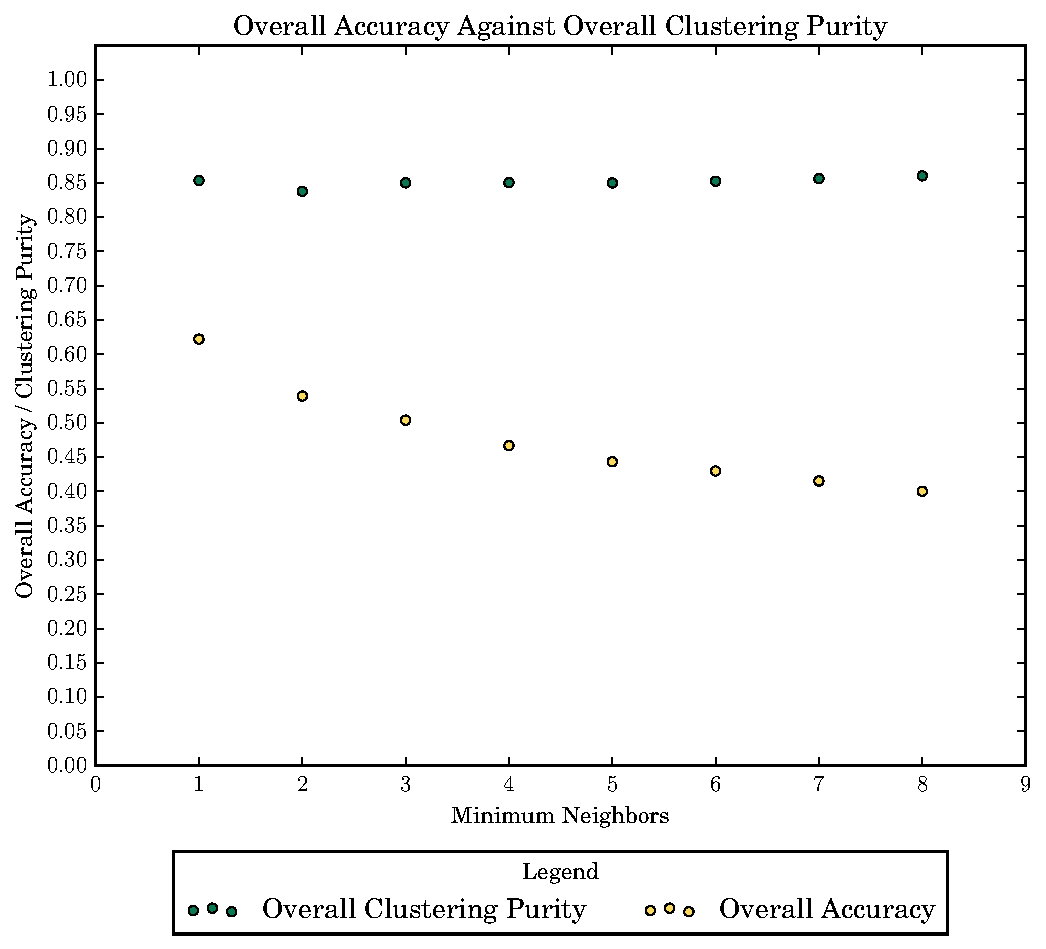
\includegraphics[width=0.75\linewidth]{figures/bs/neigh_clust_accuracy.pdf}
    %\caption{The overall accuracy decreases as we restrict  \minneigh{}. 
    %The overall clustering purity stays relatively the same as we increase the value for \minneigh{}. 
    %That is, for clustered \isols{}, the classification algorithm stays relatively the same relative to the number of isolates accurately clustered.}
    \label{fig:overall}
\end{figure}
\end{frame}
%%%%%%%%%%%%%%%%%%%%%%%%%%%%%%%%%%%%%%%%
\begin{frame}{Benefits \& Drawbacks}
Benefits
\begin{itemize}
    \item Fast --- Can cluster offline and check membership
    \item Highly pure clusters 
    \item Minimal transient strains
\end{itemize}

Drawbacks
\begin{itemize}
    \item Unknown might not be near a cluster
\end{itemize}
\end{frame}

%%%%%%%%%%%%%%%%%%%%%%%%%%%%%%%%%%%%%%%%
\begin{frame}{\Isol{}-Based Approach}

Our \isol{}-based approach:
\begin{enumerate}
    \item Find $k$ known \spec{} \isols{} from \cplop{} most similar to it, called the \knnlong{}
    \item Classify the source \spec{} of the \isol{} as the dominant \spec{} of the \knnlong{}
\end{enumerate}
Relevant computer algorithms:
\begin{itemize}
    \item The \kNNlong{} Classification Algorithm
    \begin{itemize}
        \item \alert{The \knnlong{} may not be strict enough}
        \item \alert{Can only take one distance metric}
    \end{itemize}
\end{itemize}
\end{frame}

%%%%%%%%%%%%%%%%%%%%%%%%%%%%%%%%%%%%%%%%
%%%%%%%%%% MACROS %%%%%%%%%%
\newcommand{\coordsize}{10}
\newcommand{\gridextra}{0.5}
\newcommand{\circleradius}{0.4}
\newcommand{\unknowncolor}{white}
\newcommand{\acolor}{cpgreen}
\newcommand{\bcolor}{cpgold}
\newcommand{\ccolor}{cpgreengold}
\newcommand{\unknownchar}{?}
\newcommand{\achar}{$A$}
\newcommand{\bchar}{$B$}
\newcommand{\cchar}{$C$}
\newcommand{\ac}{\color{white}}
\newcommand{\drawunknownpoint}[2]{
\draw[thick, fill=\unknowncolor] (#1) circle (\circleradius) node[] (#2) {\unknownchar}
}
\newcommand{\drawapoint}[2]{
\draw[thick, fill=\acolor] (#1) circle (\circleradius) node[text=white] (#2) {\achar}
}
\newcommand{\drawbpoint}[2]{
\draw[thick, fill=\bcolor] (#1) circle (\circleradius) node[] (#2) {\bchar}
}
\newcommand{\drawcpoint}[2]{
\draw[thick, fill=\ccolor] (#1) circle (\circleradius) node[] (#2) {\cchar}
}
\newcommand{\knngraphscale}{0.60}
\begin{frame}[t]{\kNNlong{} Classification Algorithm}
%%%%%%%%%% GRAPH %%%%%%%%%%
\begin{figure}
\centering
\pgfdeclarelayer{points} % declare foreground layer
\pgfdeclarelayer{edges} % declare foreground layer
\pgfdeclarelayer{grid} % declare foreground layer
\pgfsetlayers{grid,edges,points} % set layer order


\begin{subfigure}{0.45\linewidth}
\begin{tikzpicture}[scale=\knngraphscale, 
                    every node/.style={scale=\knngraphscale}]
    \begin{pgfonlayer}{grid}
    \draw[step=1, gray, very thin] (0-\gridextra,0-\gridextra) grid (\coordsize+\gridextra,\coordsize+\gridextra);
    \draw[thick, ->] (0,0) -- (\coordsize+\gridextra,0);
    \draw[thick, ->] (0,0) -- (0,\coordsize+\gridextra);
    \foreach \x in {1,...,10} % edit here for the numbers
    \draw[shift={(\x,0)},color=black] (0pt,0pt) -- (0pt,-3pt) node[below, fill=white] {$\x$};
    \foreach \y in {1,...,10} % edit here for the numbers
    \draw[shift={(0,\y)},color=black] (0pt,0pt) -- (-3pt,0pt) node[left, fill=white] {$\y$};
    \end{pgfonlayer}
    
    \begin{pgfonlayer}{points}
    \drawunknownpoint{5,5}{unknown};
    \drawbpoint{6,6}{one}; % 1.414 B
    \drawapoint{3,6}{two}; % 2.236 A
    \drawapoint{4,7}{three}; % 2.236 A
    \drawcpoint{3,3}{four}; % 3.000 C
    \drawbpoint{8,5}{five}; % 2.828 B
    \drawbpoint{6,8}{six}; % 3.162 B
    \drawcpoint{3,2}{seven}; % 3.606 C
    \drawcpoint{1,3}{eight}; % 4.472 C
    \drawcpoint{1,1}{nine}; % 5.657 C
    \drawapoint{1,10}{ten}; % 6.403 A
    \end{pgfonlayer}
    
    \begin{pgfonlayer}{edges}
        
        \visible<2->{
        \path[-]
            (unknown)
            edge[]
            (one)
            
            (unknown)
            edge[]
            (two)
            
            (unknown)
            edge[]
            (three)
            
            (unknown)
            edge[]
            (four)
            ;
        }
        
        \visible<3->{
        \path[-]
            (unknown)
            edge[]
            (five)
            
            (unknown)
            edge[]
            (six)
            ;
        }
        
        \visible<4->{
            \path[-]
            (unknown)
            edge[]
            (seven)
            
            (unknown)
            edge[]
            (eight)
            
            (unknown)
            edge[]
            (nine)
            ;
        }
    \end{pgfonlayer}
    
\end{tikzpicture}
\end{subfigure}
\hspace{23pt}
\begin{subfigure}{0.45\linewidth}
\small
\only<1>{
\begin{tabular}{|c|c|c|c|}             \hline
  \rowcolor{white} \k{} & Class         & Position & Similarity    \\ \hline
  \rowcolor{white}      & \unknownchar{}& (5,5)     & 0.000       \\ \hline
  %\hline
  %\rowcolor{\bcolor}  1    & \bchar{}      & (6,6) & 1.414       \\ \hline
  %\rowcolor{\acolor}  \ac2    & \ac\achar{}      & \ac(3,6) & \ac2.236       \\ \hline
  %\rowcolor{\acolor}  \ac3    & \ac\achar{}      & \ac(4,7) & \ac2.236       \\ \hline
  %\rowcolor{\ccolor}  4    & \cchar{}      & (3,3) & 2.828       \\ \hline
  %\rowcolor{\bcolor}  5    & \bchar{}      & (8,5) & 3.000       \\ \hline
  %\rowcolor{\bcolor}  6    & \bchar{}      & (6,8) & 3.162       \\ \hline
  %\rowcolor{\ccolor}  7    & \cchar{}      & (3,2) & 3.606       \\ \hline
  %\rowcolor{\ccolor}  8    & \cchar{}      & (1,3) & 4.472       \\ \hline
  %\rowcolor{\ccolor}  9    & \cchar{}      & (1,1) & 5.657       \\ \hline
  %\rowcolor{\acolor} \ac10    & \ac\achar{}      & \ac(1,10) & \ac6.403       \\ \hline
\end{tabular}
}
\only<2>{
\begin{tabular}{|c|c|c|c|}             \hline
  \rowcolor{white} \k{} & Class         & Position & Similarity    \\ \hline
  \rowcolor{white}      & \unknownchar{}& (5,5)     & 0.000       \\ \hline
  \hline
  \rowcolor{\bcolor}  1    & \bchar{}      & (6,6) & 1.414       \\ \hline
  \rowcolor{\acolor}  \ac2    & \ac\achar{}      & \ac(3,6) & \ac2.236       \\ \hline
  \rowcolor{\acolor}  \ac3    & \ac\achar{}      & \ac(4,7) & \ac2.236       \\ \hline
  \rowcolor{\ccolor}  4    & \cchar{}      & (3,3) & 2.828       \\ \hline
  %\rowcolor{\bcolor}  5    & \bchar{}      & (8,5) & 3.000       \\ \hline
  %\rowcolor{\bcolor}  6    & \bchar{}      & (6,8) & 3.162       \\ \hline
  %\rowcolor{\ccolor}  7    & \cchar{}      & (3,2) & 3.606       \\ \hline
  %\rowcolor{\ccolor}  8    & \cchar{}      & (1,3) & 4.472       \\ \hline
  %\rowcolor{\ccolor}  9    & \cchar{}      & (1,1) & 5.657       \\ \hline
  %\rowcolor{\acolor} \ac10    & \ac\achar{}      & \ac(1,10) & \ac6.403       \\ \hline
\end{tabular}
}
\only<3>{
\begin{tabular}{|c|c|c|c|}             \hline
  \rowcolor{white} \k{} & Class         & Position & Similarity    \\ \hline
  \rowcolor{white}      & \unknownchar{}& (5,5)     & 0.000       \\ \hline
  \hline
  \rowcolor{\bcolor}  1    & \bchar{}      & (6,6) & 1.414       \\ \hline
  \rowcolor{\acolor}  \ac2    & \ac\achar{}      & \ac(3,6) & \ac2.236       \\ \hline
  \rowcolor{\acolor}  \ac3    & \ac\achar{}      & \ac(4,7) & \ac2.236       \\ \hline
  \rowcolor{\ccolor}  4    & \cchar{}      & (3,3) & 2.828       \\ \hline
  \rowcolor{\bcolor}  5    & \bchar{}      & (8,5) & 3.000       \\ \hline
  \rowcolor{\bcolor}  6    & \bchar{}      & (6,8) & 3.162       \\ \hline
  %\rowcolor{\ccolor}  7    & \cchar{}      & (3,2) & 3.606       \\ \hline
  %\rowcolor{\ccolor}  8    & \cchar{}      & (1,3) & 4.472       \\ \hline
  %\rowcolor{\ccolor}  9    & \cchar{}      & (1,1) & 5.657       \\ \hline
  %\rowcolor{\acolor} \ac10    & \ac\achar{}      & \ac(1,10) & \ac6.403       \\ \hline
\end{tabular}
}
\only<4>{
\begin{tabular}{|c|c|c|c|}             \hline
  \rowcolor{white} \k{} & Class         & Position & Similarity    \\ \hline
  \rowcolor{white}      & \unknownchar{}& (5,5)     & 0.000       \\ \hline
  \hline
  \rowcolor{\bcolor}  1    & \bchar{}      & (6,6) & 1.414       \\ \hline
  \rowcolor{\acolor}  \ac2    & \ac\achar{}      & \ac(3,6) & \ac2.236       \\ \hline
  \rowcolor{\acolor}  \ac3    & \ac\achar{}      & \ac(4,7) & \ac2.236       \\ \hline
  \rowcolor{\ccolor}  4    & \cchar{}      & (3,3) & 2.828       \\ \hline
  \rowcolor{\bcolor}  5    & \bchar{}      & (8,5) & 3.000       \\ \hline
  \rowcolor{\bcolor}  6    & \bchar{}      & (6,8) & 3.162       \\ \hline
  \rowcolor{\ccolor}  7    & \cchar{}      & (3,2) & 3.606       \\ \hline
  \rowcolor{\ccolor}  8    & \cchar{}      & (1,3) & 4.472       \\ \hline
  \rowcolor{\ccolor}  9    & \cchar{}      & (1,1) & 5.657       \\ \hline
  %\rowcolor{\acolor} \ac10    & \ac\achar{}      & \ac(1,10) & \ac6.403       \\ \hline
\end{tabular}
}
\end{subfigure}
%\caption{Example graph of datapoints in a coordinate space. 
%All but one of the datapoints have a class associated with them, \achar{}, \bchar{}, or \cchar{}. 
%The class of one point, denoted by \unknownchar{}, requires determination. 
%\Compfuncs{} like \euclid{} or \manhattan{} may be the most appropriate way to compare these datapoints and \autoref{fig:knn} shows how \euclid{} and various \k{} can classify this point.}
\label{fig:knn-graph}
\end{figure}
\end{frame}
%%%%%%%%%%%%%%%%%%%%%%%%%%%%%%%%%%%%%%%%
\section{The \kraplong{}}
%%%%%%%%%%%%%%%%%%%%%%%%%%%%%%%%%%%%%%%%
\begin{frame}{\krap{}}
\begin{block}{\kraplong{} (\krap{})}
A set of four resolution strategies designed to resolve the multiple \knnlong{} lists created by multiple \compfuncs{}.
\end{block}
What we add to \kNNlong{}:
\begin{itemize}
    \item The \knnlong{} may not be strict enough:
    \begin{itemize}
        \item \a{} Filtering
    \end{itemize}
    \item Two \itsshort{} regions $\Rightarrow$ multiple \compfuncs{}:
    \begin{itemize}
        \item \rmean{}
        \item \rwinner{}
        \item \runion{}
        \item \rintersect{}
    \end{itemize}
\end{itemize}
\end{frame}
%%%%%%%%%%%%%%%%%%%%%%%%%%%%%%%%%%%%%%%%
\subsection{Methodology}
%%%%%%%%%%%%%%%%%%%%%%%%%%%%%%%%%%%%%%%%
\begin{frame}{\a{} Filtering}
The \knnlong{} may not be strict enough

\a{} Filtering Procedure:
\begin{enumerate}
    \item Query for the \knnlong{}
    \item Filter the \knnlong{} by \a{}
    \item Classify as the most dominant classification
\end{enumerate}
\end{frame}
%%%%%%%%%%%%%%%%%%%%%%%%%%%%%%%%%%%%%%%%
\begin{frame}{\a{} Filtering}
\a{} = 4.000
%%%%%%%%%% GRAPH %%%%%%%%%%
\begin{figure}
\centering
\pgfdeclarelayer{points} % declare foreground layer
\pgfdeclarelayer{edges} % declare foreground layer
\pgfdeclarelayer{grid} % declare foreground layer
\pgfsetlayers{grid,edges,points} % set layer order


\begin{subfigure}{0.45\linewidth}
\begin{tikzpicture}[scale=\knngraphscale, 
                    every node/.style={scale=\knngraphscale}]
    \begin{pgfonlayer}{grid}
    \draw[step=1, gray, very thin] (0-\gridextra,0-\gridextra) grid (\coordsize+\gridextra,\coordsize+\gridextra);
    \draw[thick, ->] (0,0) -- (\coordsize+\gridextra,0);
    \draw[thick, ->] (0,0) -- (0,\coordsize+\gridextra);
    \foreach \x in {1,...,10} % edit here for the numbers
    \draw[shift={(\x,0)},color=black] (0pt,0pt) -- (0pt,-3pt) node[below, fill=white] {$\x$};
    \foreach \y in {1,...,10} % edit here for the numbers
    \draw[shift={(0,\y)},color=black] (0pt,0pt) -- (-3pt,0pt) node[left, fill=white] {$\y$};
    \end{pgfonlayer}
    
    \begin{pgfonlayer}{points}
    \drawunknownpoint{5,5}{unknown};
    \drawbpoint{6,6}{one}; % 1.414 B
    \drawapoint{3,6}{two}; % 2.236 A
    \drawapoint{4,7}{three}; % 2.236 A
    \drawcpoint{3,3}{four}; % 3.000 C
    \drawbpoint{8,5}{five}; % 2.828 B
    \drawbpoint{6,8}{six}; % 3.162 B
    \drawcpoint{3,2}{seven}; % 3.606 C
    \drawcpoint{1,3}{eight}; % 4.472 C
    \drawcpoint{1,1}{nine}; % 5.657 C
    \drawapoint{1,10}{ten}; % 6.403 A
    \end{pgfonlayer}
    
    \begin{pgfonlayer}{edges}
        
        \path[-]
            (unknown)
            edge[]
            (one)
            
            (unknown)
            edge[]
            (two)
            
            (unknown)
            edge[]
            (three)
            ;
            
        
        \path[-]
            (unknown)
            edge[]
            (five)
            
            (unknown)
            edge[]
            (six)
            ;
        
        \path[-]
            (unknown)
            edge[]
            (seven)
            
            (unknown)
            edge[color=red]
            (eight)
            
            (unknown)
            edge[color=red]
            (nine)
            
            (unknown)
            edge[]
            (four)
            ;
    \end{pgfonlayer}
    
\end{tikzpicture}
\end{subfigure}
\hspace{23pt}
\begin{subfigure}{0.45\linewidth}
\small
\begin{tabular}{|c|c|c|c|}             \hline
  \rowcolor{white} \k{} & Class         & Position & Similarity    \\ \hline
  \rowcolor{white}      & \unknownchar{}& (5,5)     & 0.000       \\ \hline
  \hline
  \rowcolor{\bcolor}  1    & \bchar{}      & (6,6) & 1.414       \\ \hline
  \rowcolor{\acolor}  \ac2    & \ac\achar{}      & \ac(3,6) & \ac2.236       \\ \hline
  \rowcolor{\acolor}  \ac3    & \ac\achar{}      & \ac(4,7) & \ac2.236       \\ \hline
  \rowcolor{\ccolor}  4    & \cchar{}      & (3,3) & 2.828       \\ \hline
  \rowcolor{\bcolor}  5    & \bchar{}      & (8,5) & 3.000       \\ \hline
  \rowcolor{\bcolor}  6    & \bchar{}      & (6,8) & 3.162       \\ \hline
  \rowcolor{\ccolor}  7    & \cchar{}      & (3,2) & 3.606       \\ \hline
  \rowcolor{red}  8    & \cchar{}      & (1,3) & 4.472       \\ \hline
  \rowcolor{red}  9    & \cchar{}      & (1,1) & 5.657       \\ \hline
  %\rowcolor{\acolor} \ac10    & \ac\achar{}      & \ac(1,10) & \ac6.403       \\ \hline
\end{tabular}
\end{subfigure}
%\caption{Example graph of datapoints in a coordinate space. 
%All but one of the datapoints have a class associated with them, \achar{}, \bchar{}, or \cchar{}. 
%The class of one point, denoted by \unknownchar{}, requires determination. 
%\Compfuncs{} like \euclid{} or \manhattan{} may be the most appropriate way to compare these datapoints and \autoref{fig:knn} shows how \euclid{} and various \k{} can classify this point.}
\label{fig:knn-graph-alpha}
\end{figure}
\end{frame}
%%%%%%%%%%%%%%%%%%%%%%%%%%%%%%%%%%%%%%%%
\begin{frame}{\rmean{}}
\end{frame}
%%%%%%%%%%%%%%%%%%%%%%%%%%%%%%%%%%%%%%%%
\begin{frame}{\rmean{}}{Averaging the Similarity Values}
\begin{figure}
\centering
\footnotesize
\begin{tabular}{c|c|c|c|c|c}
    \k{} & \Isol{} $x$ & \Spec{} & $\pcsixt(u,x)$ & $\pcfive{}(u,x)$ & $\mathit{mean}(\pcsixt{}, \pcfive{})$  \\ \hline\hline
    1 & $a$ & \textbf<5->{Cat}  & \textit<2->{0.994} & \textit<3->{0.991} &  \textbf<4->{0.993} \\ \hline
    2 & $b$ & Dog               & \textit<2->{0.990} & \textit<3->{0.994} &  \textbf<4->{0.992} \\ \hline
    3 & $c$ & Dog               & \textit<2->{0.995} & \textit<3->{0.989} &  \textbf<4->{0.992} \\ \hline
    4 & $d$ & Chicken           & \textit<2->{0.985} & \textit<3->{0.987} &  \textbf<4->{0.986} \\ \hline
    5 & $e$ & \textbf<5->{Cat}  & \textit<2->{0.980} & \textit<3->{0.990} &  \textbf<4->{0.985} \\ \hline
    6 & $f$ & \textbf<5->{Cat}  & \textit<2->{0.978} & \textit<3->{0.990} &  \textbf<4->{0.984} \\ \hline
    7 & $g$ & \textbf<5->{Cat}  & \textit<2->{0.980} & \textit<3->{0.984} &  \textbf<4->{0.982} \\ \hline
    8 & $h$ & Chicken           & \textit<2->{0.952} & \textit<3->{0.960} &  \textbf<4->{0.956} \\ \hline
    %9 & $i$ & Chicken   & 0.952 & 0.946 &  0.948 \\ \hline
\end{tabular}
%\caption{An example classifying an unknown \isol{} \UNKNOWN{} using \rmean{} with \k{} = 8, where the mean function is the arithmetic average of the two \pcfunclabel{} values. The resulting classification is Cat.}
\label{fig:meanwise:example}
\end{figure}
\vspace{-8pt}
\rmean{}:
\begin{enumerate}
    \item Between \isols{}, average the \Ssixt{} and \Sfive{} similarity values
    \item Sort all \isols{} by similarity value
    \item Classify as the most dominant \spec{}
\end{enumerate}
\end{frame}
%%%%%%%%%%%%%%%%%%%%%%%%%%%%%%%%%%%%%%%%
\begin{frame}{\rwinner{}}{Determining the Winning Classification}
\vspace{-8pt}
\begin{figure}
\centering
\footnotesize
\begin{subfigure}{0.45\linewidth}
%\subfloat[A \k{} = 8 nearest neighbors list for the \Ssixt{} region of an unknown \isol{}.]{
\begin{tabular}{c|c}
     \k{} (\Ssixt{}) & \Spec{}  \\ \hline \hline
     1 & \textbf<2-3>{Bat} \\ \hline
     2 & \textbf<2-3>{Bat} \\ \hline
     3 & Cat \\ \hline
     4 & Pigeon \\ \hline
     5 & Pigeon \\ \hline
     6 & Human \\ \hline
     7 & Human \\ \hline
     8 & \textbf<2-3>{Bat} \\ \hline
\end{tabular}
%}
\caption{\Ssixt{}}
\end{subfigure}
\quad
\begin{subfigure}{0.45\linewidth}
%\subfloat[A \k{} = 8 nearest neighbors list for the \Sfive{} region of an unknown \isol{}.]{
\begin{tabular}{c|c}
     \k{} (\Sfive{}) & \Spec{}  \\ \hline \hline
     1 & \textbf<3-4>{Pigeon} \\ \hline
     2 & Bat \\ \hline
     3 & Cat \\ \hline
     4 & \textbf<3-4>{Pigeon} \\ \hline
     5 & Bat \\ \hline
     6 & \textbf<3-4>{Pigeon} \\ \hline
     7 & Cat \\ \hline
     8 & \textbf<3-4>{Pigeon} \\ \hline
\end{tabular}
%}
\caption{\Sfive{}}
\end{subfigure}
%\caption{In this example of \rwinner{} for \k{} = 8, \kNN{} on the \Ssixt{} region results in a classification of Bat, since there are 3 bats in its \knnlong{} list and \kNN{} on \Sfive{} results in Pigeon, since there are 4 Pigeons in its \knnlong{} list. The classification resulting from these two lists is Pigeon, since Pigeon shows up more in its original list.}
%\caption{For \rwinner{}, since there are 3 bats in \Ssixt{} and 4 pigeons in \Sfive{}, the resulting classification is Pigeon.}
\label{fig:winner:example}
\end{figure}
\vspace{-8pt}
\rwinner{}:
\begin{enumerate}
    \item Find \knnlong{} for \Ssixt{} and \knnlong{} for \Sfive{}
    \item Find the most dominant \spec{} in each list
    \item Classify as the dominant \spec{} with the highest count in its original list
\end{enumerate}
\end{frame}
%%%%%%%%%%%%%%%%%%%%%%%%%%%%%%%%%%%%%%%%
\begin{frame}{\runion{}}{Combining Both Lists}
\begin{figure}
\centering
\footnotesize
\begin{subfigure}{0.45\linewidth}
%\subfloat[A \k{} = 8 nearest neighbors list for the \Ssixt{} region of an unknown \isol{}.]{\label{fig:union:example:ssixt}
\begin{tabular}{c|c}
     \k{} (\Ssixt{}) & \Spec{}  \\ \hline \hline
     1 & \textbf<4>{Dog} \\ \hline
     2 & \textbf<2>{Human} \\ \hline
     3 & \textbf<2>{Human} \\ \hline
     4 & \textbf<2>{Human} \\ \hline
     5 & \textbf<4>{Dog} \\ \hline
     6 & \textbf<4>{Dog} \\ \hline
     7 & \textbf<2>{Human} \\ \hline
     8 & \textbf<2>{Human} \\ \hline
\end{tabular}
%}
\caption{\Ssixt{}}
\end{subfigure}
\quad
\begin{subfigure}{0.45\linewidth}
%\subfloat[A \k{} = 8 nearest neighbors list for the \Sfive{} region of an unknown \isol{}.]{
\label{fig:union:example:sfive}
\begin{tabular}{c|c}
     \k{} (\Sfive{}) & \Spec{}  \\ \hline \hline
     1 & \textbf<3>{Turkey} \\ \hline
     2 & \textbf<4>{Dog} \\ \hline
     3 & \textbf<4>{Dog} \\ \hline
     4 & \textbf<3>{Turkey} \\ \hline
     5 & \textbf<3>{Turkey} \\ \hline
     6 & \textbf<4>{Dog} \\ \hline
     7 & \textbf<3>{Turkey} \\ \hline
     8 & Cow \\ \hline
\end{tabular}
%}
\caption{\Sfive{}}
\end{subfigure}
%\caption{For \runion{}, the \Ssixt{} has 5 humans and \Sfive{} has 4 turkeys. However, both have 3 dogs, for a total of 6 dogs between the two lists. Thus, the resulting classification is Dog.}
\end{figure}
\vspace{-8pt}
\runion{}:
\begin{enumerate}
    \item Find \knnlong{} for \Ssixt{} and \knnlong{} for \Sfive{}
    \item Combine the two lists into a single list, called ``the union''
    \item Classify as the most dominant \spec{} in the union
\end{enumerate}
\end{frame}
%%%%%%%%%%%%%%%%%%%%%%%%%%%%%%%%%%%%%%%%
\begin{frame}{\rintersect{}}
\rintersect{}:
\begin{enumerate}
    \item Find \knnlong{} for \Ssixt{} and \knnlong{} for \Sfive{}
    \item Find \isols{} that appear in both lists
    \item Build a \k{}-sized list of these \isols{}, called ``the intersection''
    \item Extend both \knnlong{} lists, if necessary\footnote{stop at \a{}}
    \item Classify as the most dominant \spec{} in the intersection
\end{enumerate}
\end{frame}
%%%%%%%%%%%%%%%%%%%%%%%%%%%%%%%%%%%%%%%%
\begin{frame}{\rintersect{}}{Finding \Isols{} in Both Lists}
\begin{figure}
\centering
\tiny
\begin{subfigure}{0.45\linewidth}
    \begin{tabular}{c|c|c}
     \k{} (\Ssixt{}) & \Isol{} ID & \Spec{} \\ \hline \hline
     \textbf<4->{1} & \textbf<4->{5823} & \textbf<4->{Pig} \\ \hline
     \textbf<2->{2} & \textbf<2->{2833} & \textbf<2->{Pig} \\ \hline
     3 & 8873 & Cow \\ \hline
     \textbf<3->{4} & \textbf<3->{5939} & \textbf<3->{Cow} \\ \hline
     5 & 6156 & Cow \\ \hline
     6 & 3676 & Human \\ \hline
     7 & 7853 & Cow \\ \hline
     8 & 5331 & Cow \\ \hline
    \end{tabular}
\caption{\Ssixt{}}
\end{subfigure}
\quad
\begin{subfigure}{0.45\linewidth}
    \begin{tabular}{c|c|c}
     \k{} (\Ssixt{}) & \Isol{} ID & \Spec{} \\ \hline \hline
     \textbf<2->{1} & \textbf<2->{2833} & \textbf<2->{Pig} \\ \hline
     2 & 2916 & Cow \\ \hline
     3 & 3813 & Human \\ \hline
     \textbf<3->{4} & \textbf<3->{5939} & \textbf<3->{Cow} \\ \hline
     5 & 6854 & Dog \\ \hline
     \textbf<4->{6} & \textbf<4->{5823} & \textbf<4->{Pig} \\ \hline
     7 & 2053 & Pig \\ \hline
     8 & 8485 & Dog \\ \hline
    \end{tabular}
\caption{\Sfive{}}
\end{subfigure}
\caption{\rintersect{} searches both lists for \isols{} that appear in both in order to build a \k{}-sized list from which to classify.}
\end{figure}
\end{frame}
%%%%%%%%%%%%%%%%%%%%%%%%%%%%%%%%%%%%%%%%
\begin{frame}{\rintersect{}}{Finding \Isols{} in Both Lists}
\begin{figure}
\centering
\tiny
\begin{subfigure}{0.45\linewidth}
\begin{tabular}{c|c|c}
 \k{} (\Ssixt{})& \Isol{} ID    & \Spec{}           \\ \hline\hline
 \bf 1          &\bf  5823      &\bf Pig            \\ \hline
 \bf 2          &\bf  2833      &\bf Pig            \\ \hline
 3              &     8873      & Cow               \\ \hline
 \bf 4          &\bf  5939      & \bf Cow           \\ \hline
 5              &     6156      & Cow               \\ \hline
 6              &     3676      & Human             \\ \hline
 7              &     7853      & Cow               \\ \hline
 \textbf<6->{8}   &\textbf<6->{5331}& \textbf<6->{Cow}    \\ \hline\hline
 9              &     2189      & Cow               \\ \hline
 \textbf<2->{10}  &\textbf<2->{2053}&\textbf<2->{Pig}     \\ \hline
 \textbf<3->{11}  &\textbf<3->{8962}&\textbf<3->{Pig}     \\ \hline
 \textbf<4->{12}  &\textbf<4->{3813}&\textbf<4->{Human}   \\ \hline
 \textbf<5->{13}  &\textbf<5->{8173}&\textbf<5->{Pig}     \\ \hline
\end{tabular}
\caption{\Ssixt{}}
\end{subfigure}
\quad
\begin{subfigure}{0.45\linewidth}
\begin{tabular}{c|c|c}
 \k{} (\Ssixt{})& \Isol{} ID        & \Spec{}           \\ \hline\hline
 \bf 1          &\bf 2833           &\bf Pig            \\ \hline
 2              &    2916           & Cow               \\ \hline
 \textbf<4->{3} & \textbf<4->{3813} & \textbf<4->{Human}  \\ \hline
 \bf 4          &\bf 5939           &\bf Cow            \\ \hline
 5              &    6854           & Dog               \\ \hline
 \bf 6          &\bf 5823           &\bf Pig            \\ \hline
 \textbf<2->{7} &\textbf<2->{2053}  & \textbf<2->{Pig}    \\ \hline
 8              &    8485           & Dog               \\ \hline \hline
 \textbf<5->{9} &\textbf<5->{8173}  &\textbf<5->{Pig}     \\ \hline
 10             &    6497           & Human             \\ \hline
 11             &    9208           & Cow               \\ \hline
 \textbf<6->{12}&\textbf<6->{5331}  &\textbf<6->{Cow}     \\ \hline
 \textbf<3->{13}&\textbf<3->{8962}  &\textbf<3->{Pig}     \\ \hline
\end{tabular}
\caption{\Sfive{}}
\end{subfigure}
\caption{\rintersect{} searches both lists for \isols{} that appear in both in order to build a \k{}-sized list from which to classify. We may need to extend the original \knnlong{} list in order to do so.}
\end{figure}
\end{frame}
%%%%%%%%%%%%%%%%%%%%%%%%%%%%%%%%%%%%%%%%
\begin{frame}{The Intersection List}
\begin{figure}
\centering
\footnotesize
\begin{tabular}{c|c|c|c}
\k{} (\Ssixt{}) & \k{} (\Sfive{}) & \Isol{} ID & \Spec{} \\ \hline \hline
 2  & 1 & 2833 & \textbf<2->{Pig} \\ \hline %1.5
 1  & 6 & 5823 & \textbf<2->{Pig} \\ \hline %3.5
 4 & 4 & 5939 & Cow \\ \hline %4
 12 & 3 & 3813 & Human \\ \hline %7.5
 10 & 7 & 2053 & \textbf<2->{Pig} \\ \hline %8.5
 8 & 12 & 5331 & Cow \\ \hline %}10
 13 & 9 & 8173 &  \textbf<2->{Pig} \\ \hline %11
 11 & 13 & 8962 & \textbf<2->{Pig} \\ \hline %12
\end{tabular}
\caption{The \k{}-sized intersection formed from finding the \isols{} that appear in both \knnlong{} lists. The resulting classification is Pig.}
\label{fig:intersection:example:intersection}
\end{figure}
\end{frame}
%%%%%%%%%%%%%%%%%%%%%%%%%%%%%%%%%%%%%%%%
\subsection{Evaluation}
%%%%%%%%%%%%%%%%%%%%%%%%%%%%%%%%%%%%%%%%
\begin{frame}{Evaluation}
Experimental Technique:
\begin{itemize}
    \item Cross-Validation with Holdout
\end{itemize}
Evaluation Metrics:
\begin{itemize}
    \item Overall Accuracy
    \item For \spec{}:
    \begin{itemize}
        \item   $R$: Recall
        \item   $P$: Precision
        \item   $F_1$: $F$-Measure:
                \[
                    F_1 
                    =
                    \frac{2}{\frac{1}{P}
                    +
                    \frac{1}{R}}
                    = 2\cdot
                    \frac{P\cdot R}
                    {P + R}
                \]
    \end{itemize}
\end{itemize}
\end{frame}
%%%%%%%%%%%%%%%%%%%%%%%%%%%%%%%%%%%%%%%%
\subsection{Results}
\newcommand{\krapfigure}[1]{\includegraphics[height=0.80\textheight]{#1}}
%%%%%%%%%%%%%%%%%%%%%%%%%%%%%%%%%%%%%%%%
\begin{frame}{Overall Accuracy}{Increasing \k{}, No \a{} Filtering}
\begin{figure}[t]
\centering
\krapfigure{figures/krap/Overall-ALL-metrics-12-0_000_new}
%\caption{
%The accuracy of all classifications performed with CPLOP across the four different algorithms with $\alpha=0.00$ shows little improvement for $k>5$. 
%We look at only the percentage of correct classifications, since that value is equivalent to the precision and the recall.
%}
\label{fig:k_overall}
\end{figure}
\end{frame}
%%%%%%%%%%%%%%%%%%%%%%%%%%%%%%%%%%%%%%%%
\begin{frame}{Cows}{Increasing \k{}, No \a{} Filtering}
\begin{figure}
\centering
\krapfigure{figures/krap/Cow-ALL-metrics-12-0_000}
%\caption{There are 1838 Cow \isol{}s in CPLOP. For most resolution algorithms, we observe little improvement when $k>5$.}
\end{figure}
\begin{tikzpicture}[remember picture,overlay, shift={(current page.center)}]
    \node[align=center]   (purepoints) at (5cm,0)  {1,749 \Isols{}};
\end{tikzpicture}
\end{frame}
%%%%%%%%%%%%%%%%%%%%%%%%%%%%%%%%%%%%%%%%
\begin{frame}{Cows}{Increasing \k{}, No \a{} Filtering}
\begin{figure}
\centering
\krapfigure{figures/krap/Cow-ALL-pvr-12-0_000}
%\caption{There are 1838 Cow \isol{}s in CPLOP. Looking at the Recall as it compares to the Precision for $\alpha=0.99$ allows us to visualize the tradeoffs we make when picking a $k$ value. Labeled within each datapoint is the $k$ value at that point}
\end{figure}
\begin{tikzpicture}[remember picture,overlay, shift={(current page.center)}]
    \node[align=center]   (purepoints) at (5cm,0)  {1,749 \Isols{}};
\end{tikzpicture}
\end{frame}
%%%%%%%%%%%%%%%%%%%%%%%%%%%%%%%%%%%%%%%%
\begin{frame}{Overall Accuracy}{Increasing \k{}, \a{} = 0.00, 0.98, 0.99}
\begin{figure}[t]
\centering
\krapfigure{figures/krap/Overall-ALL-metrics-12-[-0_----0_98--0_99]}
%\caption{Shown is the accuracy of all classifications performed with CPLOP across the four different algorithms. We find that the accuracy of certain resolution algorithms perform better with higher $\alpha$ values.}
\label{fig:alpha_overall}
\end{figure}
\end{frame}

%%%%%%%%%%%%%%%%%%%%%%%%%%%%%%%%%%%%%%%%
\begin{frame}{Nonuniformity and Underrepresentation}{Chickens}
\begin{figure}[t]
\centering
\krapfigure{figures/krap/Chicken-ALL-metrics-12-0_000}
%\caption{There are 40 Chicken \isol{}s in CPLOP. Unfortunately, due to their low representation in CPLOP, classification accuracy is low.}
\label{fig:k_chicken}
\end{figure}
\begin{tikzpicture}[remember picture,overlay, shift={(current page.center)}]
    \node[align=center]   (purepoints) at (5cm,0)  {44 \Isols{}};
\end{tikzpicture}
\end{frame}

%%%%%%%%%%%%%%%%%%%%%%%%%%%%%%%%%%%%%%%%
\begin{frame}{Nonuniformity and Underrepresentation}{Cats}
\begin{figure}[t]
\centering
\krapfigure{figures/krap/Cat-ALL-metrics-12-0_000}
%\caption{There are 40 Chicken \isol{}s in CPLOP. Unfortunately, due to their low representation in CPLOP, classification accuracy is low.}
\label{fig:k_cat}
\end{figure}
\begin{tikzpicture}[remember picture,overlay, shift={(current page.center)}]
    \node[align=center]   (purepoints) at (5cm,0)  {46 \Isols{}};
\end{tikzpicture}
\end{frame}

%%%%%%%%%%%%%%%%%%%%%%%%%%%%%%%%%%%%%%%%
\begin{frame}{Nonuniformity and Underrepresentation}{Bats}
\begin{figure}[t]
\centering
\krapfigure{figures/krap/Bat-ALL-metrics-12-0_000}
%\caption{There are 40 Chicken \isol{}s in CPLOP. Unfortunately, due to their low representation in CPLOP, classification accuracy is low.}
\label{fig:k_bat}
\end{figure}
\begin{tikzpicture}[remember picture,overlay, shift={(current page.center)}]
    \node[align=center]   (purepoints) at (5cm,0)  {37 \Isols{}};
\end{tikzpicture}
\end{frame}

%%%%%%%%%%%%%%%%%%%%%%%%%%%%%%%%%%%%%%%%
\section{Conclusion}
%%%%%%%%%%%%%%%%%%%%%%%%%%%%%%%%%%%%%%%%
\begin{frame}{Conclusion}
Clustering for Bacterial Strains with \dbscan{}
\begin{itemize}
    \item Benefits
        \begin{itemize}
            \item Offline clustering and simple membership check $\Rightarrow$ \textbf{fast}
            \item Most clusters are pure
            \item Most clusters have low number of unique \spec{}
            \item Transient strains are visible and few in number
        \end{itemize}
    \item Drawbacks
        \begin{itemize}
            \item Might not classify all \isols{}
        \end{itemize}
\end{itemize}
\end{frame}
\begin{frame}{Conclusion}{\krap{}}
\krap{}:
\begin{itemize}
    \item Observations
    \begin{itemize}
        \item $5 \leq{} \k{} \leq{} 10$
        \item \a{} generally improves classification
    \end{itemize}
    \item Performance
    \begin{enumerate}
        \item \rintersect{} performed best with \a{} filtering:
        \begin{itemize}
            \item \a{} = 0.00: 74.7\%
            \item \a{} = 0.98: 78.0\%
            \item \a{} = 0.99: 85.9\%
        \end{itemize}
        \item \runion{} performs very well:
        \begin{itemize}
            \item Without \a{} filtering, it classifies best:  76.4\%  accuracy overall
            \item With \a{} filtering: minimal improvement
        \end{itemize}
        \item \rmean{}: 73.2\% overall accuracy.
        \item \rwinner{}: 65\% to 68\% accuracy
    \end{enumerate}
    \item Drawbacks
    \begin{itemize}
        \item Difficulty with underrepresented \spec{}
    \end{itemize}
\end{itemize}
\end{frame}
\begin{frame}{Conclusion}{Future Work}
Future Work
\begin{itemize}
    \item Retooling \cplop{} for automatic \mst{}
    \item Does combining these two (\kNClong{}) help \mst{}?
    \item Efficient study
\end{itemize}
\end{frame}

\begin{frame}{Questions?}
    \centering
    \Large
    Questions?
\end{frame}

\begin{frame}
\centering
\large
    This presentation was shamelessly created in 

\Huge
\rmfamily
    \LaTeX{}
\end{frame}

%%%%% CITATIONS %%%%%
\begin{frame}[t, allowframebreaks]
    \tiny
    %\nocite{*}
    \nocite{DBLP:conf/bibm/McGovernDKBVG15, DBLP:conf/bcb/McGovernJDBKV16}
    \frametitle<presentation>{References}
    \setbeamertemplate{bibliography item}[text]
    \bibliographystyle{plain}
    \bibliography{999bibliography}
\end{frame}


\end{document}
%%%%% END DOCUMENT %%%%%
%%%%%%%%%%%%%%%%%%%%%%%%%%